\documentclass[linespread=1.5]{ctexbook}

\renewenvironment{quotation}{
	\par
%	\noindent
%	%\setlength{\leftskip}{4em}
%	\setlength{\parindent}{2em}
%	\hangafter 0
%	\setlength{\hangindent}{2em}
	\kaishu
}{\newline \noindent}

\usepackage[margin=2cm]{geometry}
\usepackage{mdwlist}



\usepackage{graphicx}

\usepackage{url}
\usepackage{hyperref}

\title{\heiti{阅读、电影}}
\author{\kaishu{北方以北}}

\begin{document}

\maketitle

\tableofcontents

\chapter{书评}

\section{哲学思想类}
\subsection{《为女权辩护:关于政治及道德问题的批判》}
玛丽身为18世纪后半叶的女人,依据启蒙主义的精神,从神学出发(上帝造男人和女人)来反驳卢梭等人认为的女人应当取悦男人、应当美丽温柔、应当仅学习如何使自己更”女性化“的当时观点,认为女人应当具备理性,因此应当学习理性,需要和男人一样接受相同的教育。玛丽认为,女人可以选择男人,因而如果不接受理性教育便不能充好女人之职。
 
当时的风俗似乎鼓励女人关注感性,而认为理性令女人不再可爱。但玛丽认为,只关注感性而缺乏理性训练的女人并档真的可爱,并且有理性的男人不会也不应该只关注女人的感性。 
很难想象这是18世纪的女人的观点,这些古典的女权主义论述其实当代都可以拿来直接”反传统“了。目前社会上反智主义盛行,很多人对“女博士”指指点点,觉得“学历太高的女人嫁不出去”,这样想人的不仅男人多,很多女人受此影响也存在这样的想法,根据我的推测,一些女人可能只是眼红学历高的女人比自己聪明,试图增强自己的“竞争力”,因此大肆贬损高学历者,以显示自己的“单纯”“可爱”。这些女人只不过是男权思想的受害者而忆,她们只是利己而自私,殊不知同样的条件下,那些有脑子的男人,会倾向于选择高学历的女人作为妻子,因为她对于子女教育和家庭关系更加理性和擅长。总之,这些反智主义的想法都只是无智者或少智者的愚蠢见解而已。女人受教育不仅必要,而且是多多益善。 

这本书不仅语言流畅,逻辑性强,而且引经据典(主要是圣经和一些著名人物的论述),而且语言浪漫华丽,大量引用圣经中的比喻,反问句比比皆是,令人无可辩驳。

关于中国社会上目前的女权主义,还需要多说几句。按理讲,女权主义(或者“女性主义”“平权主义”等等,它们的内涵应当相同)是社会进步的体现,旧时代女人与男人地位明显不平等 ,抹煞了她们的聪明才智,因此社会需要把从她们那里收回来的权利还给她们。但如何还?如何平权?不同的人有不同的见解。很多人(应该都是些女人)没读过《第二性》,没看到李银河的《女性主义》,更没有就女权主义的历史演进进行研究进而结合中国实际进行理性思考,而是简单粗暴地按着字面意思来理解或被人带节奏,认为应当是给女人的利益越多越好,进而要求明显失之公平的利益。这样的言论,在微博和豆瓣上有很多,根本不需要列举。我所理解的女权主义,应当是“拉女人一把,让她们像男人那样奋斗并争取利益”,而非“坑屌丝男一把,让他们无偿并且无差别给女人更多利益”。很多女人借自己生孩子有功,向男方索要天价彩礼,在家里颐使气指,对男人百般挑剔,全然没有启蒙主义以来的理性和平等精神。更有甚者,将女权主义和消费主义捏到一起,认为女人就应当享受,借此大手大脚,不管钱是怎么挣到手的,非要把自己打扮得精致无比,或花钱享受,或寻求“诗和远方”。这些女人,其实是被商人们洗了脑,认为享乐就是平权。还有一些女人,可能是被父亲歧视,也可能是在感情里受了伤,于是产生了严重的厌恶男性的心态,把一些恶毒的词语无差别加诸男人头上,什么“拔屌无情”啊,什么“你国男人”啊,什么“宅男屌丝”啊,一个比一个难听,甚至将这上升到民族层面,认为中国男人自古如此,因而比白人男性低等,宁肯为白人男性做牛做马,也不愿看中国男人一眼。这种逆向民族主义的心态,只是感性的诉诸语言暴力,可以说和玛丽都差了很远,更不要说和波伏娃这样的准哲学家了。这些女人,把男人推向了对立面,使很多人对女权主义产生了厌恶的看法,其实无助于社会问题的解决。那些号称女权主义的女人们需要(当然男人们也需要)多读书,多独立思考,而不是撒泼打滚呼天抢地。任何权利,都是自己争取来的。想想看一百年前工人阶级争取自己的利益,流了多少血,做了多大牺牲,才换来更好的福利保障,今天的女权主义运动,不应当也如此吗?

以上这都是大错特错的想法。所谓平权,应当是像男人那样与世界战斗,而不是借舆论甚至国家力量再搞一些收入再分配。因此,从女权主义的起源,到发展,其实都是自由主义框架下的演进,都应当是个人依据自己独立的精神向世界开战。在共产主义框架内,女人根本就是和男人一样的人,能顶半边天,都是同样的劳动者。这也是为什么中国在在旧社会男女不平等十分严重,而经过共产主义革命后女人的地位上升极快,超过了作为发达国家的日本和韩国,也超过了台湾。其实在《第二性》里,波伏娃也认为工人阶级才能实现男女平等,而资产阶级(自然也包括小资们)女性难以平等,因为后者脱离了劳动,因而放弃了争取自己平等的机会。因此,根据中国的现实,努力保障女人的受教育和劳动的权利,提高生育保障,才能有效地促进男女平等。如果从宏观层面,政府的做法不宜激进,而应当努力为将来的更加平等创造条件,不能插手干涉过于微观的问题,这些都应当交给具体的个人去实现。
\subsection{《岳村政治》}
这本书2012年初买到手,当时只看了第一章前两节和附录《衡山调查记事》的三分之二,之后研究生做实验做课题,来郑州工作,忽忽四年都没有再翻开看看。2014年租房住,书放在集体宿舍,2016年七月才搬到新家。后来收拾好次卧放进书桌,这才回到灯下看书的日子。

佩服作者于建嵘为了获取第一手资料,不是坐在书斋空想,而是前后历经两年(1999-2001年)深入乡村、镇和县里实地考察,与农民、村干部、镇干部和县委交流询问,吃住在农民家里,往往需要记录写作到凌晨、坐农用车冒雨赶路,多次感冒。这种精神,恐怕不是随便一个博士生能做到的。

从行文可以看出,于建嵘是个很有情怀的人,虽为学者,但面对农民丝毫不摆架子,也有能力和农民深入交谈以获取真实想法(这在田野调查里很重要),同时又能坚持原则敢于当面拒绝不合理的请求,这一点恐怕大多数学者不会愿意做或做不了这么好。于建嵘出身农民,小时候是黑户,对农民的感情是真挚饱满的。后来于建嵘在北京画家村,进京上访的人喜欢找他,他也乐于帮助他们,又是做饭又是给钱。他写书前干过律师,还会作画,《母亲》这幅画和罗文中的《父亲》也有异曲同工之处。他给官员讲学,也乐于引导他们关注底层和弱势群体。总之,他的人格,我佩服,见贤思齐,我也要学习!

正因为深入基层,使得作者有了大量的访谈笔录、文字资料(如乡约、政府文件等)和调查问卷,对一些最基本问题有了实证性的记录(比如农民的负担、村干部的工作难处、镇政府的财政状态等),这恐怕是本书最有价值的部分。附录里的调查记录,虽然像写日记,但文字中间有推论和思考,读起来比正文的要严谨。

本书为农村社会的几千年变迁(主要是近一百年)给出了清晰的理论框架和模型,着重阐述了乡村社会在国家主导的社会制度变革中的合作及抵触,并分析了包括各级基层政府、传统宗族势力、家庭、各级干部如何共同作用于这一变革。

作者给出了农村社会的民主化方向的畅想,但结论显得仓促,缺少足够的论据。事实上,从作者完成本书(博士论文)到现在已经16年了,农村社会除了农民负担更轻、收入提高显著、更多更快的人才及劳动力流失、基层更失控、群体性事件更多以外,政治结构并没有什么变化。看来,农村的民主化社区的努力基本是失败的,城镇化才是方向。

湖南农村的发展水平,基本上比华北要快上十年。
\subsection{《虐恋亚文化》}
\subsubsection{一些标注}

西方的第一次性革命是性的解放,而第二次性革命却是从性中解放出来。

女性的虐恋幻想多为屈从和降服,而男性的虐恋幻想富于迎接苦难、自我放弃的味道。
女性的被动性心理机制是缘于其缺少适当的器官,无法发泄攻击和占领外在世界的冲动,只好将这种冲动保留在其机体内,将其自身作为攻击对象。换言之,向外在世界施虐的冲动在不可能得到发泄时,转向了内在世界。

由于权力使人感到害怕,不平等关系使人感到羞辱,所以是性感的。不平等关系能使人产生热情,因而人类性行为本身就具有权力的内涵。

欲望是人所固有的,它似乎是人的某种本质,它决定了人的某种身份;而快乐则是人的选择。虐恋到底是人的欲望还是人的选择?在福柯看来,它是人的一种自愿的选择,是人对快乐的追求。

女人比男人的内心矛盾更强烈:她们既需要解放,又需要庇护所;既需要自由,又需要压抑。

性的满足植根于权力之中。

在他的作品中,女性被残害、被强奸,为男人的快乐服务。他还曾说过,由于女性的性快感是可以假装出来的,而疼痛是不能假装的,因此对于女性来说,性活动的最高形式是痛苦而不是快乐。

权力不是一种外在的有形的机制,而是监控人的内心机制。它早已被人内化在自我之中,使人的自我成为自身欲望的劲敌。它使人害怕自己的某些欲望,甚至害怕自己的好奇心。它将人的精神锁进牢笼,不允许它自由地感觉,自由地宣泄,自由地满足它的欲望。

虐恋亚文化的出现应追溯到17世纪和18世纪,

端庄在一种文化中地位越是重要,丧失端庄、受到羞辱在人们心目中就越是可怕,从而引起过多的焦虑。虐恋中的羞辱因素是对端庄的补偿,或者说是对过度强调端庄的反动。

下山时他不能不想着爬下一座山的辛苦;而当他辛苦地往山上爬时,心里充满对下山的预期和快感。这就是受虐倾向的感觉,他在一切顺遂时感到压抑,在经受磨难时才感到愉快。

双性恋者和同性恋者参与虐恋活动的比例大大高于异性恋者。

\subsubsection{感想}

1.这本书是对SM的一个深入全面的科普对SM的形式、历史、各方关注焦点和文化社会意义进行了介绍。内容上主要是李银河引用资料(而非做实地调查),如SM的主要作者、心理学家、文化学家的论述,一些受访者的口述(当然是第二手资料),女权主义和SM爱好者的论战等等。全书是典型的学术型结构,比较好读。

2.SM不是少数爱好者的怪癖好,而是参与者的性游戏和性角色扮演。从生理上讲,鞭打拳交捆绑等等看似受虐的行为为在下着带来痛感,同事大脑分泌力比多使人产生快感。而SM更重要的是心理上的,它使受虐者在羞辱和束缚甚至奴役的状态下体验权利剥夺感,将自我心灵完全交给在上者或施虐者,体验在社会现实生活中完全体验不到的感觉,从而获得性快感。具体的心理机制是复杂的,可能跟基督教赎罪文化、抛弃自我及义务、恋物等有关。因此,SM本质上是受虐者的游戏,是施虐者服务受虐者的。

3.SM渊源极远,它和人类文明里奴役压迫禁锢相伴生,然而比较显著的影响是一些文学作品,比如萨德和马索克,比如英国维多利亚时期的地下文学,比如性革命后的广泛地下实践。不得不说英国人严肃绅士的面孔下,对鞭笞竟然有如此大的爱好。人不能太严肃,否则极易“变态”啊!

4.女权主义对SM有完全分裂的观点。激进女权主义将性固定为霸权,所以只要和性有关系,必然拖入政治领域来审视。然而,SM是私人领域的游戏,不应当拿公共领域的标尺来衡量。激进女权主义中强烈丑化反对SM的人根本不了解SM,认为它和公共领域的奴役和暴力没有区别。推崇SM的激进女权主义则为SM加入了过多进步意义。我同意SM(包括大多数不影响他人的性)和政治无关的观点。

5.从我个人来看,我是有强烈的受虐倾向的(不过SM从整体上来讲,本来就是受虐者的天堂,施虐者只不过是一个服务者,或者纯粹发泄内心愤怒的人,但他的行为应当是严格受控的。)。我有恋物癖,我喜爱丝绸,喜爱头发,喜爱皮肤,为了这种癖好,我想我可以接受轻微的虐待,比如鞭打,捆绑等等。但是,我是有女性崇拜的,必须由我崇敬的女人来打我,她至少应当强势,或者应当漂亮。我真希望我的女友能够满足我的这种癖好,否则出去找这种服务对我而言很困难。
\subsection{《动物庄园》}
1.完全是对苏联历史的寓言式讽刺,熟悉苏联历史会在里面找到列宁、斯大林、托洛斯基等人的原型,也能看出“其他庄园”里代表的那些“帝国主义”国家。

2.从本书里并不一定能推论出“社会主义一定坏”,只能推出“那几只猪都是
\subsection{《送你一颗子弹》}
文气贯通,一气呵成,如同听善谈者讲故事讲“道理”,中间几篇文章,讲婚姻感情的讲生活琐事(特别是奇特的胃口的)读起来尤其利索爽快。

收录的多是博客,都是生活中的一些感受体会,杂乱琐碎。没有政论文章。其实刘瑜有“民主女神”的称号在外,又是政治学的博士,政论文章应该更有价值。看完我想翻翻她的博客看看她的民主和政治高论了。

总得说吧,从这些文字里,不难看出刘瑜是个活得很自在很丰富的知识分子,思想独立,在感情上有追求有一定品味的女人。写字有点话痨,生活不超过书斋和起居饮食之外,圈子小,格局不大,稍显空泛,与人交往不强势也不弱势,离人群有点远,有点书呆气。
\subsection{《共同的底线》}
秦晖这本书写于90年代到2005年左右,出版时是2013年,到现在已经有20年了,但对事实的判断皆为真知灼见,读之获益颇多。

\subsubsection{关于主义}
主义满天飞,但秦晖的这张图把各种思想和主义的源流清晰地表达出来: 
\begin{figure}[htpb]
\centering
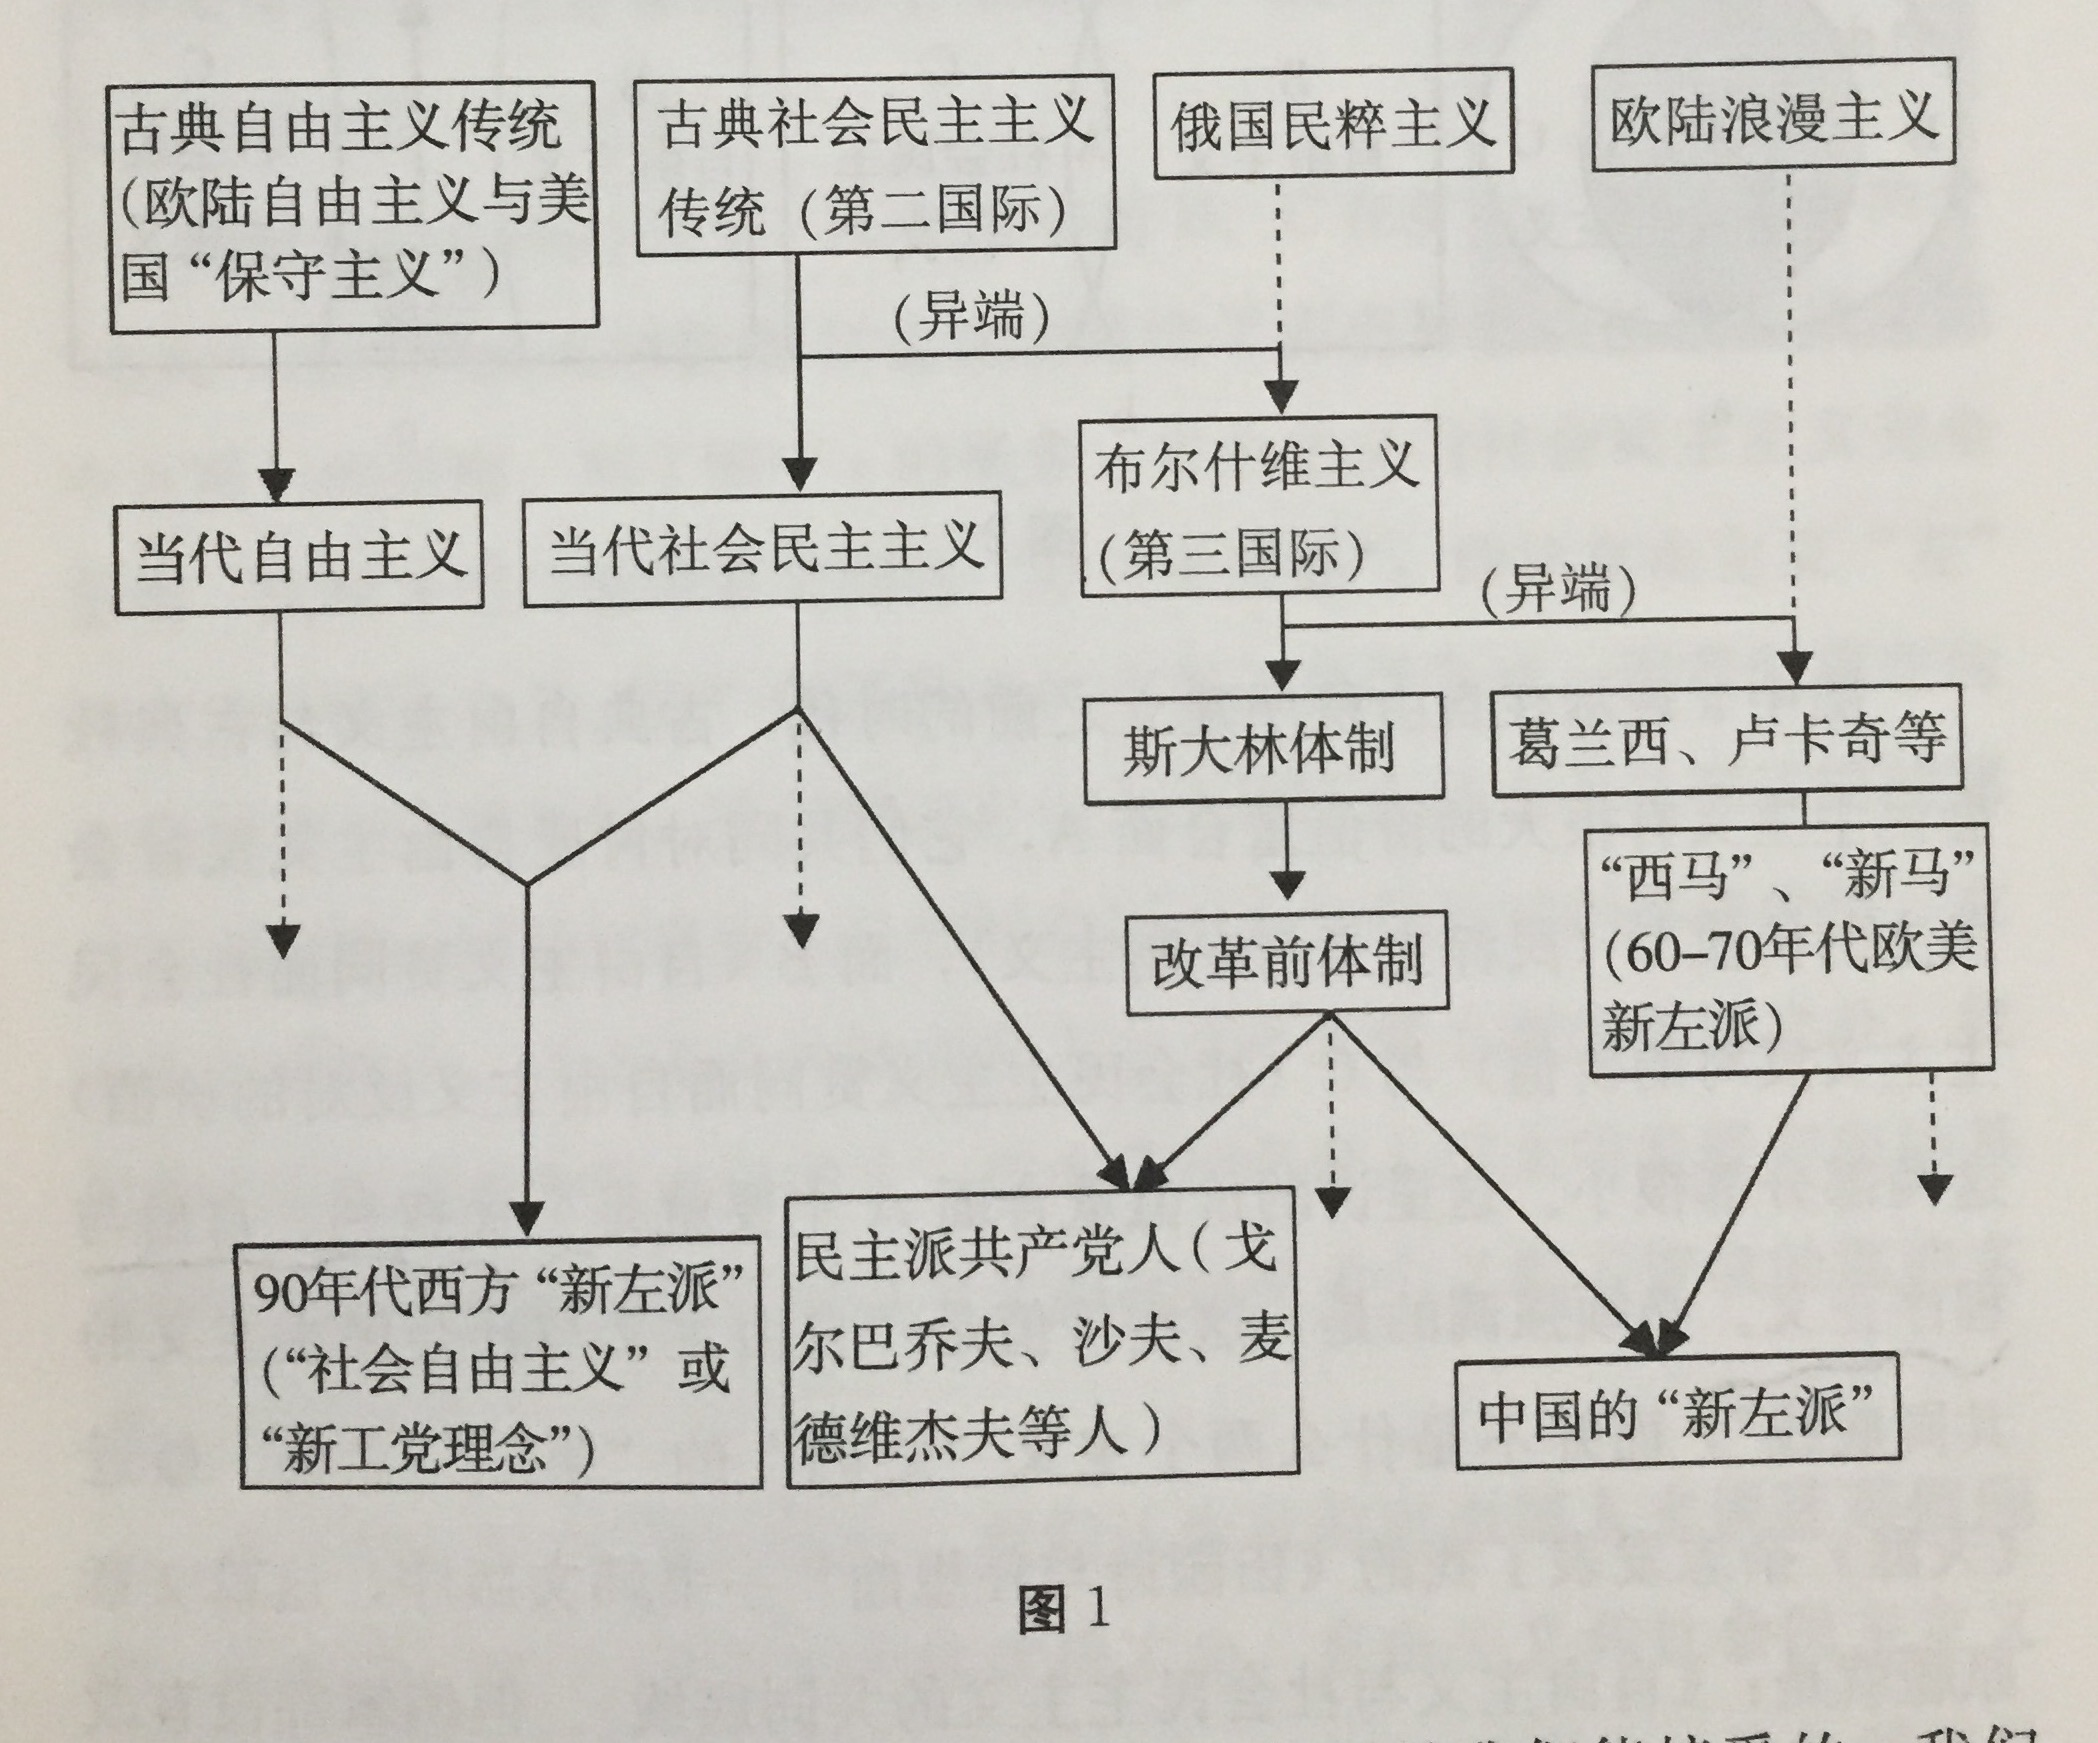
\includegraphics[width=0.5\linewidth]{images/zhuyi.jpg}
\end{figure}
以及
\begin{figure}[htpb]
\centering
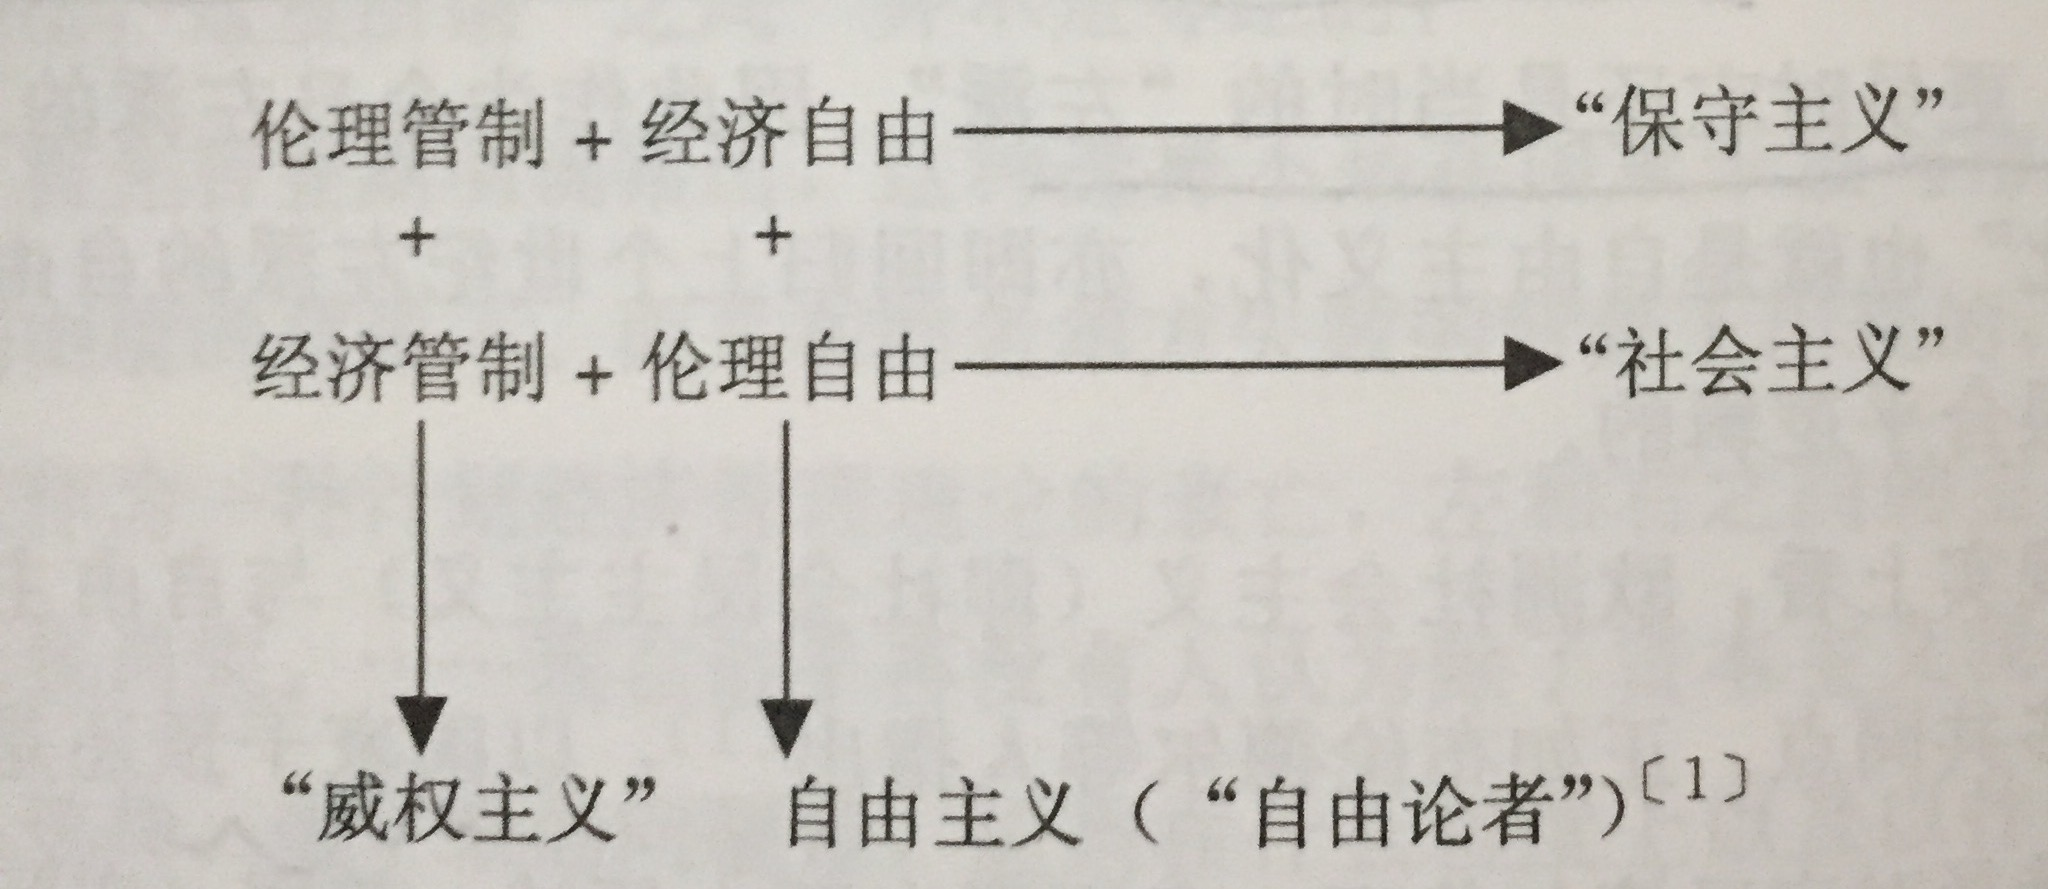
\includegraphics[width=0.5\linewidth]{images/zhuyi2.jpg}
\end{figure}

秦晖是自由主义者,认为自由主义“一个基本内容就是强调‘群己权界’。公域讲民主,私域讲自由”。

宪政的目的就是要使政府的权力与责任相对应,这种权力必须为被统治者所授予,而授予的唯一目的就是要政府能够向被统治者负责。宪政与民主是两回事,前者追求权责对应,后者追求多数决定。前者讲的是权力运用的规则,后者讲的是权力的来源。无民主则宪政原则不能贯彻到底,无宪政则民主机制更会走向反面。 
\begin{figure}[htpb]
\centering
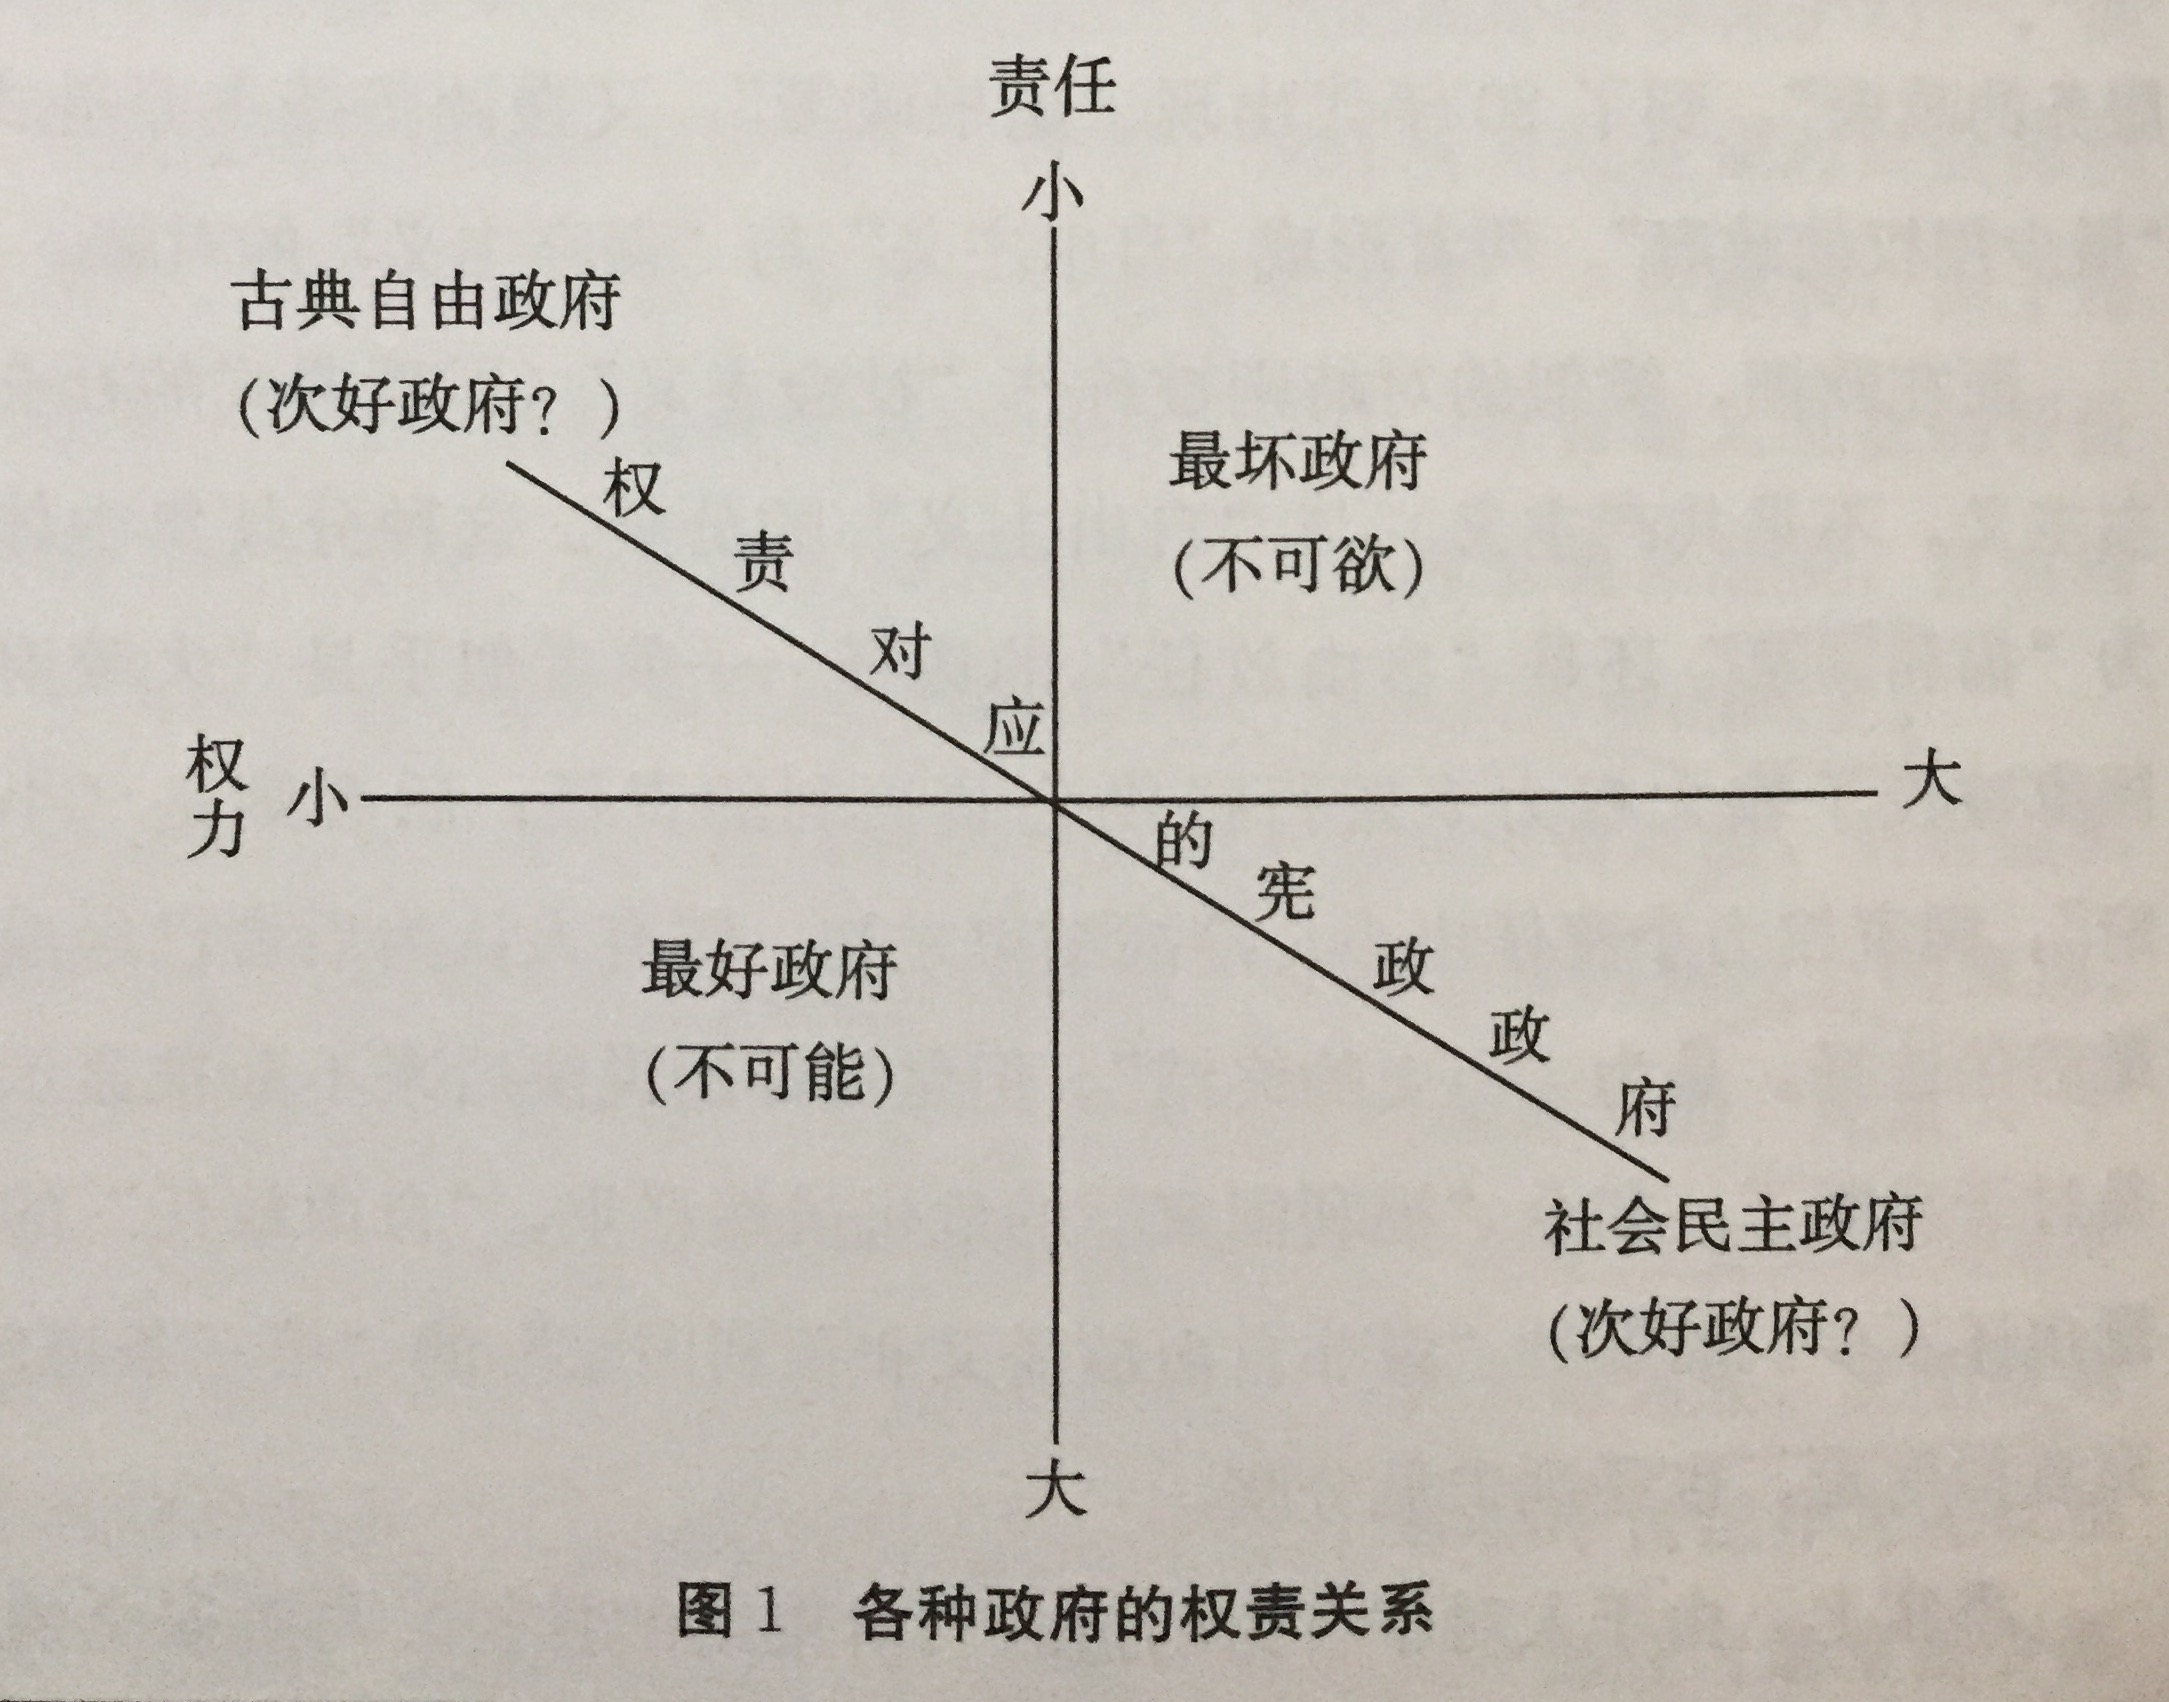
\includegraphics[width=0.5\linewidth]{images/zhengfu.jpg}
\end{figure}

为了捍卫公正,哈耶克主张可以引申为\emph{过程公正,既往不咎},诺齐克主张\emph{过程公正必咎既往,原则上可以一直追溯到”最初获得“}。

\subsubsection{关于俄国革命}
俄国十九世纪末二十世纪初的改革和随后而来的革命是中国革命的样板。这段时间内:
\begin{quotation}
俄国民粹派一方面极言知识分子的虚伪、委琐与农民的朴实、崇高,甚至提出“知识分子应当拜倒在农民脚下”,但另一方面又强调束缚农民,所说农民一旦“脱离土地,忘记‘务农’,那么俄国人民、人民的世界观、人民发出的光和热便不复存在,剩下的只是空虚的灵魂、‘完全的自由自在’、可怕的‘爱上哪儿就上哪儿’”。
\end{quotation}
这是随后斯大林时代的文字注脚,同时被我党学过去,成为直至现在的文艺指导方针。

\subsubsection{关于中国的改革}
\subsection{《乌合之众》}

1.这本书并不是一部真正的心理学著作,通篇没有严谨的论述,没有科学的推理,只有片段的观察和武断的判断。因此它只是一本通俗读物,不应该把它当成严肃的社会心理学的学术著作。有趣的是,作者反对的群体性弱点里,那些“乌合之众”恰恰喜欢领袖们这样的论断。

2.由于缺乏严谨的论述,因此看这本书决不能被作者的论断吓住,要思考究竟对不对,特别是反例是否存在,从当前例子能否必然得到当前结论。

3.作者语言极富于煽动性,如果你对这本书的观点全盘接受,那么你也会成为不会思考的乌合之众。

4.作者对群体缺乏思考的论断我严重不同意,它举的例子,如中世纪的欧洲和法国大革命,往往是由于当时某个群体的信息闭塞和科技落后导致的,或是缺乏科学态度。当然,群体行动力和思考力的严重不一致我是同意的,群体即是法律我也极为认同,但群体的盲目并不是这些因素的必然结果。

\emph{(待续,目前只看了全书的前百分之二十)}

5.作者似乎对“民族性”或“国民性”相当看重,认为这是一个国家民众的生活习惯,影响这个国家的政治制度和行为。比如,作者反复提到的法国人的冲动易于煽动,影响着法国的近代历程,特别是法国大革命和1848年波旁王朝的复辟。

6.作者对法庭和议会这样的“乌合之众”指责颇多,即使它们都是受到教育的人的集合,但在愚蠢和易于煽动上和没受到教育的人一样。作者警惕议会制度会因为议员为自己前程着想会过多增加选民福利,从而增加政府规模和权利,反过来会限制公民自由,这在战后成为了现实。

7.虽然如此,但作者坚定维护民主制度,认为这是最不坏的制度。

8.作者对社会主义表示警惕,认为这种把理想放在现世的宗教,会在它建立的那一刻便开始消亡。不得不说,这个论断还是很精准的,特别是对列宁主义这一派。

9.总之,作者是个有远见和极度聪明的人,但书中观点是不是正确,恐怕是仁者见仁智者见智的事情了。反正,我对耍聪明讨论严肃问题又缺乏严谨论证的书,评价不高。亚马逊上给了三星评价。
\subsection{《沉默的大多数》}

\begin{quotation}
缺少科学知识,没有想象力,这都是中国出不了科幻片的原因,
\end{quotation}
这么多年过去了,王小波的说法还是很正确。

尤其是理科的男学生,肯定希望在校园里出现一些表演系的女生??这很有必要。

中国传统的士人,除了有点文化之外,品行和偏僻小山村里二十岁守寡的尖刻老太婆也差不多。

中国有种老女人,面对着年轻的女人,只要后者不是她自己生的,就要想方设法给她罪受:让她干这干那,一刻也不能得闲,干完了又说她干得不好;从早唠叨到晚,说些尖酸刻薄的话--捕风捉影,指桑骂槐。

第三个假设是凡人都喜欢有趣。这是我一生不可动摇的信条,假如这世界上没有有趣的事我情愿不活。有趣是一个开放的空间,一直伸往未知的领域,无趣是个封闭的空间,其中的一切我们全部耳熟能详。

一部《情人》曾使法国为之轰动。大家都知道,这本书的作者是刚去世不久的杜拉斯。这本书有四个中文译本,其中最好的当属王道乾先生的译本。我总觉得读过了《情人》,就算知道了现代小说艺术;读过道乾先生的译笔,就算知道什么是现代中国的文学语言了。
作者看这部小说说不错,我觉得的一般。

真正有出息的人是对名人感兴趣的东西感兴趣,并且在那上面做出成就,而不是仅仅对名人感兴趣。

人和人其实是很隔膜的。有些人喜欢有趣,有些人喜欢无趣,这种区别看来是天生的。

\section{心理情感类}
\subsection{《男人这东西》}
\subsubsection{感想}

1、看完渡边淳一的这本《男人这东西》,深深为日本男人感到悲哀:男主内女主外的经济状态很难改变,工作压力极大,与妻子的交流产生了莫大的障碍,导致性功能低下。

2、作者描述的是日本,想必是对日本社会、尤其是婚姻家庭有大量的观察总结才做出的,即使作者没有做严谨的社会学调查和数据统计分析,但身为日本人,又是作家,对日本社会的观察应该还是站得住脚的。但是,这种观察结论能否适用于中国社会呢?我想这是需要打一个问号的。比如,日本普遍(根据作者的语气,应该90\% 以上)男主内女主外,家庭主妇相当普遍,但在中国,男女共同工作(早些年的“双职工”)现象相当普遍,因此男女经济社会地位相对而言更对等,因此像日本的那种夫妻双方分工明确的现象没有那么严重。

3、日本男人可怜的自尊心:日本男人认同更强,因此拼命想做到更强,但竞争激烈,大部分人仍旧是平庸的,这产生了大量的沮丧情绪,而日本男人在家里又想维持一种高高在上的心态,对妻子强迫命令,这各矛盾心态造就了日本男女之间那种尊卑关系。虽然日本经济发达,女权运动比中国要早,但男女截然不同的经济命运和强大的心理传统造成了男女之间的差别越来越大。

4、作者认为,男人的生理结构决定了只有在“高高在上”的情况下才能勃起并有性能量,而现代社会的竞争机制使以往男女之间的能力差异迅速缩小,甚至在少年时代被女生吊打,因此男人的自尊心受到极大的“损害”,从而导致性功能障碍。失意的男人为找回“自尊”,在婚恋时更希望找到愿意做家庭主妇的人来弥补这种挫败感,因此男主内女主外的传统更难打破。

5、在作者笔下,男人是脆弱的可怜的,特别是处于激烈竞争环境下的男人,需要和女人做心理上的比较和对抗,忙于工作,逃避家庭,任凭自己在酒精的刺激和烟花女子的抚慰下堕落。对此我只想说:你们不能改变吗?这种稳定的日本社会不能发生自发的变化并朝向对男女双方都有利的方向做出修改吗?作者的答案似乎是:不能,我们日本人难以改变。

6、日本的女权状况不会比中国更好,这不是由经济发展水平决定的,而是由强大的传统和习俗决定的。同样,本书的分析未必适用于中国社会。中国的职业状况,会朝着西方学习,而不会退回到男人必强女人必弱的旧时代去,因此中国相比日本,更接近西方。

7、在作者笔下,日本男人尽管可怜,可又相当固执,非要在女人面前保持好胜心,用比较的方式来证明自己的优越和对方的差劲。亦即,日本男人的心态是:你有各种各样的缺点,因此就别在我面前逞强了,乖乖臣服于我的命令吧。当然,可以想见,日本女人也会有同样的心理。这样,男女双方都在一种”比比谁更差劲“并且以羞辱对方并打击对方自尊心的方式来交流的。想想这样的交流方式其实相当可怕。我不知道日本社会人与人的关系是否都如此,然而根据作者描述,日本的男女关系就是对上述心态的演绎。因此,日本男人要么不是直男癌,如果是,一定比中国男人更接近晚期。

8、作者鉴于男女关系在一夫一妻制对男女双方个性的压制,极力推崇日本平安时代的”走婚“形式,即女性保持多个男性伴侣的婚姻。虽然作者也说日本的社会不允许这种婚姻,但在我看来,即使允许,恐怕也不能解决男女关系的种种问题。走婚并不是多么稀罕的东西,中国西南某少数民族即有这种形态,但婚姻不仅仅是男女关系的问题,其实是一种经济形态,是在保证血缘关系前提下最灵活同时最稳定的经济小集团。走婚,或者不婚,虽然可以保证男女在年轻时的性欲望得到最大满足,但一旦老去,将难以解决晚年的生活问题。概而言之,只有一夫一妻制,才能以最小的成本来保证双方一生的生活水准。

\subsubsection{一些标注}

希冀爱情的人最好对结婚打消期待,而希冀结婚的人最好对恋爱打消期待——

男人和女性属于不同的群组,从本质上说是无法真正相互理解的,

在近代小说中,恋爱的精神性被推到了最前沿。

近现代的男女之爱表现出浓烈的禁欲主义色彩,

(日本)即使是因妻子感情出轨而离婚,丈夫也不得不支付高额的赡养费,而如果因丈夫有外遇而离婚,妻子则只需给极少的赡养费。

女性的筑巢本能强于男人

夫妻之间保持一定的距离感、紧张感,有利于彼此保留一份新鲜感,双方互需互求,这样或许可以减少男人的花心。

没有血缘之亲的父母和子女之间,永远都不可能真正理解,

但对男人来说,他们所期待的家庭无非是一个不必设防、能够彻底放松身心的场所,失意时能够得到抚慰,屈辱时能够得到鼓励,使其第二天继续鼓足干劲儿投入到工作中去。

男人本身是一个非常社会性的存在,

女人想最终称心如意地得到心仪的男人,最有效的办法莫过于抓住他的心理脆弱之处。
男人如果失去友情便意味着被男性社会屏弃在外,最终成为一只失群的孤狼,这也意味着男人将彻底被这个社会抛弃。男人早在少年时期就开始体会到这种感觉,所以在男性社会中确保自己的位置对他们而言,同珍视自己的妻子或女友一样重要,绝对是不可或缺的。 这种倾向在日本的男性社会里尤其明显,如果对男人的这种感觉不能理解,也就无法真正地理解男人和女人。

对那些依靠女人养活的倒贴男人,社会上一般都称之为“吃软饭的”,竭尽蔑视,而反过来对于依靠男人养活的女性,则呼之为“妻子”,正儿八经地予以认可。

与女性相比,男人在性爱中所得到的快感是一种浅层次的快感,而且不可能随着精神之爱的逐渐深化而加深或变得更强烈,故此对男人来说,同某个特定的女性的性爱在他们身上很难刻下深刻的烙印。

\section{经管类}
\subsection{《当代中国经济改革教程》}
作者:吴敬琏

这是一本\emph{一本运用现代经济学的分析工具考察中国改革的著作}。

标注:
\begin{itemize*}
	\item 匈牙利经济学家科尔奈早就论证过,计划经济是一种短缺经济。也就是说,它的常态是总需求远大于总供给。不过,由于在计划经济体制下绝大部分商品实行固定价格制度,需求过旺和供给不足通常并不表现为价格上涨,而是在行政压制下隐性地存在着,并以配给制度和额外的寻求成本等形式表现出来。
	\item 从短期的观点看,在1978年末改革开放以来30年的时间里,中国宏观经济引人注目的特征是反复出现经济过热和通货膨胀。
	\item 凯恩斯主义宏观经济政策的主张是,当出现总需求不足和经济萧条的情况时,用扩张性的宏观经济政策增加总需求来加以救助;反之,当出现了总需求过旺和经济过热的情况时,则主张用紧缩性的宏观经济政策减少总需求来加以抑制。
	\item 一位卫生部前副部长指出,中国政府投入的医疗费用中,80%用于党政干部。
	\item 在计划经济条件下,传统社会主义国家社会保障的典型特征是政府直接向社会成员提供实物福利,而不是像在市场经济条件下那样,主要是建立针对某些风险的福利维持计划。
	\item WTO 规定(1)缔约一方给予任何一方的优惠,也给予所有缔约方;(2)缔约方之间相互保证给予对方的自然人、法人和商船与本国自然人、法人、商船相同的待遇(国民待遇);(3)缔约一方不得对任何缔约方实施歧视性待遇,要使所有缔约方能在同样的条件下进行贸易;(4)关税是WTO所认可的唯一合法保护方式,缔约各国应不断降低关税的总体水平;等等。
	\item 为什么进口替代的工业化不能像预期的那样发挥作用呢?根据克鲁格曼的分析,最重要的原因是:发展中国家制造业发展程度低下,通常是由于缺乏熟练的劳动力,企业家、管理人才和社会组织方面存在问题等多方面的原因造成的;贸易保护政策非但不能为这些国家的制造业创造出竞争力,相反会使这些部门和企业效率下降。而且,进口替代战略还会因为给予少数受到保护的精英企业获得垄断利润的特权,而使二元经济及收入分配不均和失业等问题加剧。
	\item 增值税的转型改革主要围绕两个方面进行:一是由生产型增值税转为消费型增值税,二是扩大增值税覆盖范围。
	\item 20世纪90年代初期,开发预算外收入已成为从中央到地方的普遍现象。到1996年末,中央政府明文规定的收费项目有130多项。经过地方政府和主管部门的层层加码,到县和县级市一级的不完全统计,各种收费项目已达1000项以上,各种基金420项以上。1992年预算外资金达到3854.92亿元,为当年全国财政收入的110.67%。
	\item 增值税不同于所得税,它是一种间接税,它的纳税人并不是税负的最终承担者。增值税的特点是对产品在其生产过程每个阶段的价值增值征税。
	\item 在各种税种中,将维护国家权益、实施宏观调控所必需的税种划为中央税;将同经济发展直接相关的主要税种划为中央与地方共享税;将适合地方征管的税种划为地方税。
	\item 美国财政学家奥茨(Wallace E. Oates)指出,财政联邦制在具备如下三个前提条件时,明显优于其他分权体制:(1)当地方政府提供该产品的成本小于中央政府,且不存在负的外部性的时候;(2)采取财政分权制度提供某种公共物品带来的福利增进与该物品的需求弹性成反比;(3)这种福利增进也与居民的迁移性成正比。
	\item 亚当·斯密在《国富论》中提出的税收四原则,即平等原则、确定原则、便利原则和经济原则,是对税收原则最系统和完整的表述。
	\item 在市场经济条件下,公共财政的基本职能,就是为政府向社会提供公共物品筹措和分配资金。
	\item 投机对于市场的有效运作有它不可或缺的作用。【216】这是因为,如果金融市场上只有长线投资者,市场就没有流动性,价格也不能被发现。投机者寻求风险收益使交易得以连续进行。但是问题在于,投机活动只有在与投资等活动结合在一起,实现良性互动时,才能够透过证券市场实现资本资源的优化配置,从而对经济起积极作用。单纯的投机炒作并不能提高效率和增加财富,只不过是“钞票在不同人的口袋之间搬家”的零和博弈【217】,
	\item 股市合规性监管最重要的职能,就在于通过强制性的信息披露制度,缓解信息不对称的问题,保护投资者的利益不受侵犯。
	\item 现代经济学认为,股票市场的基本功能是通过股市交易和股价变动,使资本资源流向效率较高的地方,实现资本资源的优化配置;与此同时,利用股价对公司绩效的度量作用,对公司经营作出评价并对经理人员进行监督。
	\item 作为资本市场分析基准(Benchmark)的MM定理【208】指出,在满足信息完全对称等一系列假设的条件下,企业的市场价值与它的融资结构无关。但在现实经济生活中的信息不对称条件下,不同的融资方式对企业市场价值的影响是不同的。
	\item 中国经济改革的第二个阶段以增量改革为基本特征。所谓增量,在很大程度上是指在原有国民经济中逐步增添新的非国有的经济成分。
	\item 作为公共企业,国有企业不管是否上市,其透明度都应该达到上市公司的水平,国有企业巨额利润不经财政预算程序而自动转为投资资金,是近年来中国经济增长过度依赖投资而消费增长乏力的一个重要原因。
	\item 1998年以后,中国政府采取了分拆改组的办法来打破垄断,形成竞争局面。
	\item 市场经济国家更普遍采用的个体农户与市场的对接形式,其实是在农业产前、产中、产后服务的各个环节上建立农民合作组织。
	\item 农业生产资料价格的上升幅度却远远超过农产品价格的上升水平。只有农业部门的剩余劳动力都被工业部门所吸收,农业部门劳动者的工资才会提高,整个经济才会转入现代增长。
	\item 制度变革本质上就应该是整体推进的,虽然在实施上可以分步进行,否则就会存在巨大的制度运行成本。
	\item 由于计划经济的资源配置方式在本质上要求集权,分权的计划经济是较之集权的计划经济还要糟的计划经济。
	\item 直到1976年“文化大革命”宣告结束,由于存在社会主义只能采取行政命令配置资源这样的意识形态障碍,市场取向改革很难在政治上被接受,向地方政府下放计划权力几乎成了唯一可能的改革选择。(1)1958~1978年:行政性分权,改革的重点是中央政府向下属各级政府放权让利。(2)1979~1993年:增量改革,改革主要在国有部门以外的经济领域中推进,并以民营经济的成长壮大来支持和带动整个国民经济的发展。(3)1994年至今:整体推进,以建立市场经济体系为目标进行全面改革。
	\item 在马克思和恩格斯看来,社会主义之所以会取代资本主义,源于资本主义社会中生产力和生产关系之间,即社会化的生产力和资本主义私人占有制度之间的冲突。
\end{itemize*}
\subsection{穷爸爸富爸爸}

\subsubsection{一些标注}
\begin{itemize*}
	\item 在如今的美国,教师工会是所有工会中最大、最富有的一个。
	\item 如果想学习销售技能,最好进一家网络营销公司,也被称为多级营销公司。这类公司多半能够提供良好的培训项目,帮助人们克服因失败造成的沮丧和恐惧心理,这种心理往往是导致人们不成功的主要原因。
	\item 如果要破产的话,一定要在30岁以前,他的建议是“这样你还有时间东山再起”。贫穷和破产的区别是:破产是暂时的,而贫穷是永久的。
	\item 财富是将资产项产生的现金与支出项流出的现金进行比较而定的。财富就是支撑一个人生存多长时间的能力,或者说,如果我今天停止工作,我还能活多久?
	\item 害怕在公众面前说话是因为害怕被排斥、害怕冒尖、害怕被批评、害怕被嘲笑、害怕被别人所不容。简言之,是害怕与别人不同。这种心理阻碍了人们去想新办法来解决问题。
	\item 资产是能把钱放进你口袋里的东西。 负债是把钱从你口袋里取走的东西。
	\item 工作只是面对长期问题的一种暂时的解决办法。
	\item 一个人一旦停止了解有关自己的知识和信息,就会变得无知。
\end{itemize*}

\subsubsection{书评}
美国的所谓“畅销书”完全就是圈钱之作,写作质量令人作呕。

这本书作为一本投资理财的启蒙读物,还是有一些干货的,比如现金流和资金流,资产与负债的区别等,也给出了一种“成为富人”(并没有!)的方案,比如购置资产坐等升值并找机会赚一笔、捡漏、少用信用卡这样的负债手段、不要只安于“眼前的苟且”而不思进取等等。

但是,本书除了这些干货,完全就是一坨狗屎。作者以自己亲身经历说明,自己是如何“背叛”自己的高级知识分子和中产阶级的”穷爸爸“的老路并如何被同学的做生意的”富爸爸“来教导并成才的。作者出身于夏威夷,貌似是日本人后裔,但白手起家,身家到写书时至少为几百万美元。作者的经历完美诠释了美国人骨子里的实用主义和功利主义。可能美国人不全是拜金的,比如小所就裸捐,但很显然一大部分人(比如像作者这样)还是把金钱看成第一位的。

作者在字里行间表现出对”穷爸爸“的鄙夷与不屑。以金钱的观看来看,”穷爸爸“确实不值那么多金钱,但一个大学教授的价值能用金钱来衡量吗?或许作者的爸爸只是一个能力一般的教授,但传道授业解惑,为人师表,决不是几百万美元能够衡量的。作者表现出的对知识和精神追求的无知令人讨厌。相反的,作者洋洋自得地述说自己赚钱的生意经,似乎自己就是唯一成功的,并且似乎只有自己这一处成功方式,这也是我所不齿的。事实上,作者行文中的缺乏逻辑和写作技巧,让人怀疑这是他口述并让秘书写成的,并不是自己的认真的作品。作者在嘲笑有技能的中产阶级,但实际上,有知识有文化的中产阶级也会嘲笑作者的无知与狂妄。

总之这本书完全不值钱。如果你想知道这本书想讲什么,还是看一些关于投资启蒙的博客和书评更好些。
\subsection{《经济学原理(马歇尔)》}
翻译还不如狗屎,错别字遍地都是,语句没一句通顺。封面上推荐说是“任何人都能读懂的经济学名著”,我看是任何人都读不懂才对。

这本书已经正式准备弃了,作为门外汉和初学者还是看曼昆的更适合

\section{文学类}
\subsection{《秘密》}
\subsubsection{一些标注}
\begin{itemize*}
	\item 写实与无情是体现作家东野圭吾创作理念的关键语。
	\item 他嫉妒重走青春的直子。他嫉妒能与直子一同享受青春的年轻男孩。同时,他也憎恨自己不能对她产生爱情与情欲。
	\item 了解他之前所不可能知道的事情。 原来是这样啊!从藻奈美口中说出许多连她原本不可能知道的事,像是平介与直子的第一次约会…… 果然,与其说藻奈美的性格变得与“直子完全相同”,还不如说是直子的人格附在藻奈美身上,这样比较容易让人接受。 平介快速地浏览了这本书。结果,他发现在“附身”这个单元之后,便是“多重人格”了。他仔细阅读了一下,其中提到几个实例,都是说明当这种现象无法用心理学的角度来解释时,就
现在的社会已经趋向高龄化了。到时候退休年龄可能已经提高到六十五或七十岁了呢!
\end{itemize*}

\subsubsection{书评}
一个看似很感人,实际上充满了人性自私的故事。不过,大概所有的感人都是人的自私在作祟。 
在一次司机疲劳驾驶的回乡之旅中,平介的妻子女儿发生事故,奇迹的是妻子直子虽然去世,但灵魂转移到女儿藻奈美体内。度过了一段不适应后,直子做了一个决定,以女儿藻奈美的身体生活,在外(主要就是学校)扮演努力学习成绩优异的藻奈美,在家扮演妻子,让自己有一个不后悔的人生(直子是家庭主妇,只上过社区大学,应该是个学渣)。平介当然是支持的。 
但随着直子升入私立女中和高中,平介无法忍受这既是女儿又是妻子、既不是女儿又不是妻子的直子了。他身体有性欲,但无法通过外貌是女儿的妻子来解决。为了事情不败露,他又没有找妻子的打算。但是,刚过四十的平介显然感觉到了自己的衰老,恐惧和孤独不断腐蚀着他的内心。他嫉妒直子,为什么她就可以“抛弃”丈夫重获青春活得有滋有味而自己却要独自承受这种人生的荒谬呢?终于,这种不满在直子将要和高中学长出去私会时达到高潮。平介探知他们的行踪,在家里装窃听器来偷听他们打电话,并最终在他们约会地点阻止了这场幽会。 
另一方面,平介也通过自己的渠道来获取真相。司机多年前有段婚姻,但婚姻里的儿子不是自己的。司机爱着这个不属于自己的儿子,虽然离婚再娶,但当这个儿子要上大学需要花钱时,通过加班和疲劳驾驶来多挣钱并汇钱给他们,终于酿成苦果导致一车人丧生,除了直子。真相很简单。 
绝望的直子又扮演起了藻奈美的角色,平介也决定以女儿的心态对待直子。但当他第一次叫直子“藻奈美”时,女儿的意识复活了。似乎直子和藻奈美共享了藻奈美的身体,五年后女儿的意识突然复活,每次醒来就要轮替意识。之后,藻奈美的意识越来越长,而直子的意识越来越短。最终,在初遇的公园里,直子的意识完全消失。 
结尾处,藻奈美和司机的儿子结了婚。失去妻子和女儿的平介想打司机儿子来泄愤,但却蹲下号啕大哭。实际上,通过藻奈美戴上了直子的婚戒,平介已经知道了其实直子没有消失,而是继续扮演着藻奈美的角色生活了下去,这成了他们两人之间的“秘密”。

其实关于换了意识的“藻奈美”究竟是直子还是藻奈美,很多人有不同看法。两者都能说通,都震撼人心。但我更喜欢“直子扮演藻奈美”的猜想。处在两难境地的平介,其实是这一群着最痛苦的人。他需要养活直子,但得不到直子的身体,因为那个身体是藻奈美的;当藻奈美“复活”,他了同时失去了女儿。平介嫁女时的心态,有女儿的父亲们应该都心有戚戚,女儿也是父亲的小情人啊!

不过,我想吐槽的是,其实需要这么痛苦吗?有着熟女内心和萝莉身体的“直子”,不是所有男人的梦想吗?这简直是通往新世界的大门啊!难道不能在一起做那种事情吗? 
而且,即使有痛苦,不能和直子坦诚交流吗?为什么苦着自己呢?

电影版由广末凉子主演,把藻奈美从小学直接搬到了高中,也取消了司机后妻的设定,直接让藻奈美遇见了司机的儿子。故事变得更简单了,取消了悬疑元素,几乎成了一部纯感情片,与原著相距甚远。因此,电影版的情节变得有点支离破碎,内心戏大幅减少,表演流于表面。可是,广末凉子好美啊!
\subsection{《情人》}
\subsubsection{标注}

我知道,女人美不美,不在衣装服饰,不在美容修饰,不因为施用的香脂价钱贵不贵,穿戴珍奇宝物、高价的首饰之类。我知道问题不在这里。问题究竟何在,我也不知道。
人家常说,我这头发最美,这话由我听来,我觉得那意思是说我不美。

\subsubsection{读后感}

1.杜拉斯的行文絮絮叨叨絮絮叨叨絮絮叨叨(重要的事情说三遍),从遇见情人的穿着到情人给她讲自己的故事,从脾气怪异的母亲(我的总结)到不争气的两个哥哥,再到遇见的几个白人朋友,东拉西扯,颇为意识流。老实说,我不喜欢这样的文风,她的文采我也丝毫不欣赏。

2.作者以讲述情人的理由,不断温习回顾自己年轻时的心态经历,回顾自己的亲人和朋友。这乃是一部回忆录。 
3.杜拉斯的讲述是啰嗦的,口语的,仿佛你在听一位年老妇人讲述自己的青春。

4.这本小说是王小波极力推崇的,他称赞杜拉斯写小说的手法独树一帜。另外,他推荐王道乾的这个译本。翻译地确实不错。

5.我不懂女人,所以这本充满女性气息的小说,我看不懂。满分五分,我给三分。
\subsection{《呼兰河传》}
\subsubsection{评论}

萧红的文字大气,很耐看。

团圆媳妇,令人悲伤,令人绝望。

磨坊里的歪嘴

贫穷封闭的生活让人变得麻木冷漠

\subsubsection{一些标注}

他不但没有感到绝望已经洞穿了他。因为他看见了他的两个孩子,他反而镇定下来。他觉得在这世界上,他一定要生根的。要长得牢牢的。他不管他自己有这份能力没有,他看看别人也都是这样做的,他觉得他也应该这样做。

等我生来了,第一给了祖父的无限的欢喜,等我长大了,祖父非常的爱我。使我觉得在这世界上,有了祖父就够了,还怕什么呢?虽然父亲的冷淡,母亲的恶言恶色,和祖母的用针刺我手指的这些事,都觉得算不了什么

是凡在太阳下的,都是健康的,漂亮的,拍一拍连大树都会发响的,叫一叫就是站在对面的土墙都会回答似的。

人若老实了,不但异类要来欺侮,就是同类也不同情。

温顺也不是怎么优良的天性,而是被打的结果。甚或是招打的原由。
\subsection{《饥饿游戏》}
\subsubsection{关于原著小说}

1.革命不是请客吃饭,也不是真人秀,但在小说里却是。小说意在讽刺电视娱乐,顺便黑了一下革命宣传,前者在第一部和第二部里是主线,后者在第三部里才图穷匕现。前两部里我期待革命者会发动苦大仇深的人命推翻凯匹特统治然后建立人民民主专政政权实现共产主义……哦不,是资本主义,但其实革命者和反革命者的套路相同,宣传工具和手段如出一辙,只不过凯匹特用恐惧的杀人游戏,革命者用高大全的革命文艺。到了凯匹特的总统府对决,革命者不惜炸死总统府前的儿童并嫁祸总统来达到自己的“革命”目的。一切革命都是反革命。看来科林斯不仅反对娱乐至上,更反对乌托邦,甚至反对一切政治,把所有革命宣传事业黑了个底朝天,这可是青少年文学啊,美帝的花朵看这种东西真的没关系吗?还能开心地投选票吗?

2.因为是给青少年看的,所以情节比较简单,也比较拖,但第二部太行文太仓促。心理描写一大段一大段,反复无常,看得人昏昏欲睡。

3.情节漏洞太多,不知道作者是不是对社会不熟悉还是故意要把社会描述地简单一些,整个帕纳姆的经济不合理,科技很发达但产业很落后,比如都能用基因工程改造动物了还用得着用人力搞农业渔业和矿产吗?

4.恋爱就是请客吃饭,但凯特妮丝和皮塔的感情,一直没看懂。皮塔为什么喜欢上凯特妮丝就不说了,凯特妮丝对皮塔的感情让人琢磨不透,凯特妮丝你真的这么高贵冷(leng)艳(dan)吗?另外对盖尔的感情让人缺乏共鸣。其实,与书中政治的弱智相比,几个主人公的年龄写得都有点大了:盖尔才多大啊去当游击队长(二区鄛匪司令?)?

5.翻译显的语言显得稚嫩,好多地方直译,不知道是不是也是要给青少年看?

\subsubsection{关于改编电影}

大表姐的表演还算可圈可点,第一次看是2013年年底在北京看第二部,特别惊险刺激。 
2017年3月8日终于刷完了最后一部,把这个系列划上了句号。 
电影不错。 
可惜电影最后生生把Snow洗白了,成了Kitness的知音。杀死了总统于是就实现了民主,这设定也太幼稚。
\subsection{《白夜行》}
1.恶只能产生更大的恶。如果不是桐原他老爸有特殊嗜好,如果不是他把魔掌伸向贫穷的雪穗母女,便不会产生这一系列令人扼腕的悲剧。

2.桐原他老爸把魔掌伸向雪穗,因为她们家穷,因为她们家软弱,但当时觉得软弱的人,多年之后变得异常强大——不,那个时候雪穗就已经很强大了。今天软弱,不代表永远软弱。

3.雪穗母亲没有尽到母亲的义务,本质上是个皮条客,拿女儿身体挣钱。家长失职,带给孩子的是永远的伤害。

4.桐原亮司的强大令人钦佩,其早熟也让人惊讶。杀父后桐原已经是一个大人了,似乎有某种更深刻的意味。

5.桐原亮司虽然自尽,但他是带着他的“白日”离开这个世界的。

6.桐原亮司一直在为被他杀害的父亲赎罪。可是,为了赎一个人的罪,把伤害带给不相关的人,是更大的恶行,这罪愆越赎越多。所以,我丝毫不同情他。

7.雪穗的犯罪“技术”丝毫不比桐原亮司弱,她善于利用人,这是犯罪最好的技术,也是这个世界最强大的技术。

8.桐原亮司死后,雪穗会有何种结局?所有的线索都已经断开,老刑警不能再追查下去,当事人死的死伤的伤,大概雪穗会继续开店,控制筱冢康晴,并最终控制筱冢家族?不过筱冢一成是她的老对手,对她的了解相当深,而她自己又失去了桐原亮司这个重要搭档,遇到拦路虎谁给她除掉?顶多也就是总裁夫人这个结局吧?自己的店倒是会开下去,搞不好会成为女装大鳄。不错的结局。

9.什么是真正的优雅?什么是真正的贵族?雪穗的优雅陶冶,骗过了这个世界的所有人,却独独骗不过真正高门大户的筱冢一成,为什么?如果说家庭的陶冶能让人从细节甚至直觉上区分别人和自己是不是一类人,那一成的堂兄康晴为什么没有这个能力?筱冢家族的其他人为什么没有这个能力?可见在东野笔下,这是某个人的一种特殊能力。一成能从雪穗的猫眼中看出她身上不属于贵族的那种狡黠和狠毒,算是这部小说的一个后门吧?果然还是富贵人看富贵人比较准,但等等,为什么康晴没有看出来呢?果然一成是雪穗的知音啊!

\subsection{《解忧杂货店》}

封面就说这不是一本推理小说,读下来才知道,虽然不是推理小说,但耗费的脑细胞并不少,交叉变换人物视点叙事本来就需要记住前面的情节和暗示,其阅读“难度”其实是比作为推理小说的《梦幻花》要高的。 
其实整个读下来,这本小说的核心就在于“时间机器”的设置,几个人的命运在浪矢杂货店和丸光园中交汇重合,又远离,然后再次汇集。 
其实这种小说没有太大的深度,读完也觉得是推理小说的皮,但核心是一碗鸡汤。

\subsection{《梦幻花》}

说实话读完这本小说有点失望,感觉作者和能写出《白夜行》和《嫌疑人X的献身》不是一个人。其实想想,这本小说的叙事技巧并不比前两者差,只是立意不高,强行为国民上课(关于核能和”家庭责任“)。为什么读下来没有前两者好?因此这本小说灌注的感情远远差于前两者。你读不出作者强行编故事渲染出的那份感动。 
小说只有三个视角:一心破案以与儿子交流的警察下濑,被父亲强行棒打鸳鸯而耿耿于怀的下治(?),以及放弃奥运梦想表哥爷爷相继被杀的秋山??。整个故事就是个一本道,前面的铺垫作者马上就迫不及待地揭开,不需要读者费脑筋。 
真相让人大跌眼镜。堂堂大日本帝国,对于疑似毒品的东西不是派个研究机构秘密保护起来,而是交给警察和医生家族,美其名曰”家族责任“。家族承担得起一国毒品滥觞之责任吗?

不过大夏天的读完两本小说确实还算满足。东野圭吾还是好好加油写出个经典出来吧!如果只是整天写一些水平低的小说,虽然赚钱多,但后世留不了名啊! 
东野圭吾的小说时间跨度大,而且有很强烈的年代感,用特定年代的一事一物就把年代传达出来,笔墨精炼,但类似猜谜语的快感还是让人兴趣盎然。
\subsection{《蒋勋说红楼梦》}
贯穿全书的题眼是“青春”。

1.青春的理解

2.告别青春以后
\subsection{《阿勒泰的角落》}
\subsubsection{感想}

1.母女两人在荒凉纯朴的新疆阿勒泰,随着牧民的迁徙而游走,卖小商品,给人裁衣服……

2.看到哈依娜一节,李娟写到她和哈依娜由陌生到朋友的转变,以及成为朋友的那种“尴尬”,突然明白了李娟田园牧歌逐草而居的生活,和喧嚷嘈杂的都市生活的区别在哪里?在哪里呢?在于她的生活很空旷,星星点点却都是珍贵的东西,她处在自己喜欢和欣赏的物体的包围里。而都市人呢,处在各种喜欢的不喜欢的层层叠叠水泄不通的包围里,都市人离不开这种包围和它带来的物质,离不开这种丰富带来的享乐。他们希望自己身边不喜欢的那些,要么通通消失,身边只剩下让自己开心的那些东西,要么成为自己喜欢的,所以他们羡慕李娟的快乐和单纯。但是,物质的丰富和物质的俗厌从来就是硬币的两面,不可能去除一面而完整保留另一面。所以,李娟的生活再美好再单纯,也不过是满足心理的空虚罢了。但是,能在复杂的生活外阅读这样的文字,对生活本身而言,已经是非常好的弥补了,这大概也是读书的价值所在吧。

3.李娟的妈妈和姥姥都是很精悍的女人,特别是李娟的妈妈,保留着巨大的童心,爱折腾,又是修窗户又是养金鱼,冒着严寒大老远带来花去养。但她不会养,能力不高,虐待金鱼,这点让我讨厌。

4.李娟在“新版自序”中说,她写下这些纯真快乐的文字时的感情,在后来的生活里已经失去了很多,所谓的“纯真与朴素”,已经慢慢失去。李娟说,“刻意地保持纯真,这本身就不是一件纯真的事吧?”难得的诚实。如果在纯真和诚实之间选择,我更喜欢后者的李娟。

\subsubsection{一些标注}

在阿克哈拉恋爱多好啊!尤其在秋天,一年的事情差不多已经忙完,漫长而悠闲的冬天无比诱惑地缓缓前来了……于是追求的追求,期待的期待……劳动的四肢如此年轻健康,这样的身子与身子靠在一起,靠在蓝天下,蓝天高处的风和云迅速奔走。身外大地辽阔寂静。大地上的树一棵远离一棵,遥遥相望。夕阳横扫过来,每一棵树都迎身而立,说出一切。说完后树上的乌鸦全部乍起,满天都是……在遥远的阿克哈拉,乌伦古河只经过半个小时就走了,人活过几十年就死了,一切似乎那么无望,再没有其他任何可能性了。世界寂静地喘息,深深封闭着眼睛和心灵……但是,只要种子还在大地里就必定会发芽,只要人进入青春之中就必定会孤独,必定会有欲望。什么原因也没有,什么目的也没有,我妹妹就那样恋爱了。趁又年轻又空空如也的时候,赶紧找个人和他(她)在一起——哎,真是幸福!

我妹妹刚满十八,已经发育得鼓鼓囊囊,头发由原先的柔软稀薄一下子变得又黑又亮,攥在手中满满一大把。

缺乏野外捕食的经验,加之天气一天冷似一天……后来第一场雪下了,第二场雪也下了……看不到一个人,得不到任何救助,然后就什么也不能明白地死去了!\footnote{可怜的狗!——读者注}

这样的山野里会有什么毒物呢?这开阔的,清新的,明亮干爽的,高处的……一眼望过去,万物坦荡,不投阴影。\footnote{有毒的很多哦!——读者注}

当他们喃喃自语地在草丛里寻找什么东西,当他们把一颗完全能够一口就吞下的糖分成无数次耐心吮完,当他们互相之间有条有理地谈论着在我们听来乱七八糟的话题……小孩子的幸福多么宽广!

其实我们这里的所有孩子都会弹电子琴的,他们好像天生就对音乐、对音阶高低的细微变化敏感异常,刚刚听完一首歌,顺手就可以在琴上完整地敲出来。

\subsection{《一个女子恋爱的时候》}
1.富家女父亲猝逝,欠下一屁股债,昔日父亲好友垂涎美色,先是温情款款让她来家居住,后来藏掖不住威逼利诱不还钱就必须嫁给她。富家女愤然离开,一直瞒着未婚夫,当掉父亲遗产住在小旅馆,找中介投资试图以三百块一年内赚十万还债(牛市冲天),发现中介也是图谋美色,又愤然离开当游轮女主人,到古巴见到父亲又一好友,回来后没钱还债,和未婚夫的感情眼看将要破解,正要被迫嫁人突然父亲好友拜访说你父亲有股份给你留了十五万,后来几位蜀黍当着坏叔叔的面揭穿了阴谋,钱还是富家女的。富家女喜见未婚夫并成婚,皆大欢喜喜大普奔。按情节就一不入流小说。

2.教训:(1)男人要慎重交友,有人对你好不一定是真的好,还有可能看上了你女儿。(2)股市有风险,投资需谨慎,一不小心就可能把女儿卖了。(3)女孩纸要谨防各种蜀黍。(4)奋斗什么的看起来很燃很鸡血,但最后的钱,还是亲爹的。

3.邹韬奋翻译不错,没有翻译腔,流畅自然,撮其大意,前几回的译后注有个人体会挺好看。

4.译后记:会说话的人能轻声讲重话,不会说话的人一出口便闹。诚哉斯言!

5.丁恩阴险,但并不猥琐,起码给了富家女贞丽起码的尊重。如果本故事走暗黑系套路,那么贞丽将死无葬身之地。

6.“在此僵局之下,尼尔珠莉和她自己三人皆感着苦痛,与其如此,不如让珠莉与尼尔能成眷属,自己宁愿牺牲;三人同苦,不如让两人快乐而只留一人痛苦。她想到这样的意境,妒意为之消除殆尽,心神反为之一爽。”从来对这种女性对情敌谦让的心态无感,如刘若英唱那句“看着她走向你,那幅画面真美丽;如果我哭泣,也是因为欢喜”,太假,太做作。

7.译者言“西谚谓“天助自助者”,我请改一字,说“人助自助者”,必先努力自助,而后人助乃得加入,若自暴自弃之徒,旁人见之,只有“爱莫能助”。”确实如此,虽然贞丽庸碌大半年啥也没干,但起码撑下来了。“机会诚若可遇而不可求,但只有最能努力者始能利用,则断然无疑。”诚哉斯言!

\subsection{《台湾单车旅行笔记》}
\subsubsection{一些标注}

上海的街道就是用中国省份和都市来命名的:南北纵向用省份,东西横向用城市。

因为“走路太慢,开车太快,而骑单车速度刚刚好……”

看北京夜景的最佳位置是香山山顶,空气清透的日子,等太阳落山,看二环、三环、四环、五环的路灯逐格点亮,

将台湾原住民分为9个族群,分别是阿美族、泰雅族、赛夏族、排湾族、布农族、卑南族、鲁凯族、邹族和达悟族,后经台湾当局修订,再加上撒奇莱雅、噶玛兰、太鲁阁、赛德克和邵族共14个族群,人数约40多万,占全台湾人口2\% ,在花莲和台东县,便有8个原住民部族。

十里青山行画里,双飞白鸟似江南。

挑战乳酸的感觉,有如吸毒一样,让你欲罢不能。

视野开阔的人,从不沉湎于痛苦或者其他糟糕的情绪,因为他能看到影子的边界,知道没有永远停留的绝望。

浊水溪,不只是一个地理名词,它不但分隔了台湾北部和台湾南部,还分隔了政治上的泛蓝和泛绿,分隔了“本省人”和“外省人”,分隔了国民党和民进党,也分隔了台湾的政声人心。

现在的台湾,铁路分为台铁和高铁两个相对的概念,前者包括了7条环岛干线(纵贯线、台中线、屏东线、宜兰线、北回线、台东线、南回线)和4条支线(平溪线、内湾线、集集线、沙仑线),后者仅有一条,即台北至高雄采用日本技术的“新干线”。

全世界第一位以双脚徒步、骑车,完成环球壮举的勇士,是中国的潘德明。

壮游要具备:明确地自我期许,要有超人的智慧。

\subsubsection{读后感}

《台湾单车旅行笔记》,文笔很稚嫩,脱不了学生腔,特别是“眼睛默黑得像……”和“看上去很平和”这样的描写不知所云,完全没有必要,根本没有传达给读者有用的信息。

鸡汤太多,没有来由的感叹太多。 鸡汤不是不能喝,而是里面要有肉,有干货。《台湾环岛旅行笔记》里,让人羡慕的不是作者随处而发的感想,而是里面的真人真事,是各人之间实实在在的温情付出。

我关心的是事实,是真实的见闻,并希望作者以直接翔实的语言表达出来。

突然对骑行有兴趣了,以后搞搞吧。让人对旅行感兴趣,或许是一本成功的旅行书的目的。
\subsection{《嫌疑人X的献身》}
1.所谓女神,不过都是女屌丝。

2.不知道这本书能否折射出日本人的性格,或者在何种程度上折射出这种性格,即压抑,隐忍,报恩,以及牺牲。那种为了所爱之人奋不顾身献身的人,不就是所谓的武士道吗?
3.故事节奏没的说,一气呵成让人不忍心合上书,结局反转很震撼。人物关系简单。是个优秀的故事。

4.好的小说不会仅仅讲一个好故事,情节取胜的,看完一遍就很难读第二遍。把人写好才能让人难以忘怀。石神对花岗靖子的爱压抑而深厚,虽然自我毁灭让人惋惜,但想想他这样的人,做出这种事不会让人惊讶,似乎也是必然。只可惜,搭了无辜人的一条命。

5.相比之下我更喜欢《白夜行》,后者更黑暗,但……
\subsection{《失魂雪》}
是一个系列,不过故事基本是独立的。故事本身还是挺吸引人的,我两天时间就读完了。


\subsection{《萧红散文选集》}
其实这不是萧红的散文集,只不过是汇总了萧红写的十几篇文章,其中最后一篇回忆鲁迅的篇幅就占去了全书的40\% 多。总的来说,萧红的文笔,写《呼兰河传》那样的小说,会让人眼前一亮,但写散文的话,结构太松散,文笔显得晦涩很多。萧红对穷人是很同情的,这大概是把她划分为左翼的原因。


\subsection{《西游记》}

\subsubsection{标注}
常言道,长安虽好,不是久恋之家。待我们有缘拜了佛祖,取得真经,那时回转大唐,奏过主公,将那御厨里饭,凭你吃上几年,胀死你这孽畜,教你做个饱鬼!

老沙原系凡夫,因怕轮回访道。云游海角,浪荡天涯。常得衣钵随身,每炼心神在舍。因此虔诚,得逢仙侣。养就孩儿,配缘姹女。工满三千,合和四相。超天界,拜玄穹,官授卷帘大将,侍御凤辇龙车,封号将军。也为蟠桃会上,失手打破玻璃盏,贬在流沙河,改头换面,造孽伤生。幸喜菩萨远游东土,劝我皈依,等候唐朝佛子,往西天求经果正。从立自新,复修大觉,指河为姓。法讳悟净,称名沙僧。

猪先世为人,贪欢爱懒。一生混沌,乱性迷心。未识天高地厚,难明海阔山遥。正在幽闲之际,忽然遇一真人。半句话,解开业网;两三言,劈破灾门。当时省悟,立地投师,谨修二八之工夫,敬炼三三之前后。行满飞升,得超天府。荷蒙玉帝厚恩,官赐天蓬元帅,管押河兵,逍遥汉阙。只因蟠桃酒醉,戏弄嫦娥,谪官衔,遭贬临凡;错投胎,托生猪象。住福陵山,造恶无边。遇观音,指明善道。皈依佛教,保护唐僧。径往西天,拜求妙典。法讳悟能,称为八戒

悟空解得是无言语文字,乃是真解。”

杨木性格甚软,巧匠取来,或雕圣象,或刻如来,装金立粉,嵌玉装花,万人烧香礼拜,受了多少无量之福。那檀木性格刚硬,油房里取了去,做柞撒,使铁箍箍了头,又使铁锤往下打,只因刚强,所以受此苦楚。

自家思虑道:“我若没本事化顿斋饭,也惹那徒弟笑我,敢道为师的化不出斋来,为徒的怎能去拜佛。”

周天之内有五仙,乃天地神人鬼;有五虫,乃蠃鳞毛羽昆。这厮非天非地非神非人非鬼,亦非蠃非鳞非毛非羽非昆。又有四猴混世,不入十类之种。”菩萨道:“敢问是那四猴?”如来道:“第一是灵明石猴,通变化,识天时,知地利,移星换斗。第二是赤尻马猴,晓阴阳,会人事,善出入,避死延生。第三是通臂猿猴,拿日月,缩千山,辨休咎,乾坤摩弄。第四是六耳猕猴,善聆音,能察理,知前后,万物皆明。此四猴者,不入十类之种,不达两间之名。

如来笑道:“汝等法力广大,只能普阅周天之事,不能遍识周天之物,亦不能广会周天之种类也。”

心高不认天家眷,性傲归神住灌江。

又有四个大天师来奏上:“太上道祖来了。”玉帝即同王母出迎。老君朝礼毕,道:“老道宫中,炼了些九转金丹,伺候陛下做丹

凡诸仙腾云,皆跌足而起,你却不是这般。我才见你去,连扯方才跳上,我今只就你这个势,传你个筋斗云罢。

一日,祖师登坛高坐,唤集诸仙,开讲大道,真个是天花乱坠,地涌金莲。妙演三乘教,精微万法全。慢摇麈尾喷珠玉,响振雷霆动九天。说一会道,讲一会禅,三家配合本如然。开明一字皈诚理,指引无生了性玄。
\subsection{骆瑞生《我的第一个以及最后一个恋人》}

这是作者在豆瓣上发表的一个连载,被我录在一块并在kindle上看完了。故事很简单,高中的农村男生和城市女生之间的恋爱故事。小说的出彩处是对农村出身的“我”的自卑、要强的心理描写,以及面对青涩的爱情时那种手足无措和悉心呵护(作者身上有我的影子)。结尾有点狗尾续貂,不过中学时的爱恋,大多都没有好结尾,一切的美好都将将留在心底,并再也不会重来。


\subsection{《红楼梦》}
这是第十来次看《红楼梦》了吧,之前没有完整地看过脂批,这个版本里脂批比较全,对各个版本的整理也算精当。脂砚斋对曹雪芹创造的“捧”占了脂批大部分,另外还有对于创作的一些看法和对过往生活的感叹,这对缺失后三四十回的《石头记》来说是不可多得的资料,红学家也大多在这个地方下功夫去考证佚失的底本。

1.王夫人这个人,极愚蠢极专制(愚蠢的人更容易专制,而且是愚蠢的专制,非开明的专制)。对待晴雯这种漂亮风流的女子极为严苛。我最讨厌这种人。

2.宝钗是儒家最欣赏的女子。我不是很喜欢儒家,但也不讨厌。儒家在社会管理上也有称道之处的,讲得清权利与义务,并用权责把人固定在一个固定的位置。宝钗学识极厚,会戏会画,以淑女自许,“珍重芳姿昼掩门”。但宝钗虽有学养但无灵气,风姿远不及黛玉,风流远不及湘云。同时宝钗有管理才能,察人心之细远过探春,阴柔手段远超凤姐。

3.黛玉之灵,甚得我心。《红楼梦》读得粗疏的,往往认为黛玉刁钻小性,这是受宝黛爱情里的儿女之态所误,试问哪个女孩在男友面前不是刁钻小性的呢?事实上在“金兰契互剖金兰语”前,因为有宝钗的存在,黛玉以为她心里藏奸,喜欢抓住金玉良缘这个问题来试探宝玉;在宝钗袒露心胸后,黛玉便视宝钗为亲姐姐,甚至薛姨妈后来住在潇湘馆照顾黛玉,形同母女,十分亲密,钗黛毫无嫌隙可言。另外,“识分定情语梨香院”后,宝玉为龄官所感,心中已有黛玉为唯一感情托付,两人不会为金玉良缘所惑,在此后的感情虽然不再浓墨重彩,但愈加深笃,如历生死。黛玉为人,大概娇柔有余而强力不足,但不至于小性。另外,下人虽更爱宝钗,但以林黛玉之聪慧,又加贾母深爱,也不至于有愤恨之意。紫鹃对黛玉之深情,比之亲姐妹更加亲密,试忙玉一节可证。这种深情,在宝钗和莺儿之间肯定看不到。黛玉之灵秀,乃是极深情极敏感,有诗人气质,作者曹雪芹行文之间,难掩偏爱之情。

4.晴为黛影,但这次看书,对晴雯实在爱不起来,她太直白太尖利,个人对袭人麝月的平稳温柔更加喜爱。

5.《红楼梦》是柔弱的,是追悔的,甚至是消极的。


\subsection{《三体》}
三体是一流的想象,二流的文笔,和三流的人物塑造。人物塑造之所以差,是因为这本书几乎把力量都放在了情节上,留给人物本身的东西并不多,也可能是大刘不善于描画人物,并以人物性格和际遇来推动情节发展。说实话,从人物那时说出来的话,除了史强这样的糙汉子外,其他那些科学家、知识分子、政府官员几乎一模一样,丝毫没有体现出人物的职业和性格特点。甚至于知识分子的思考,也都是大刘硬加给他们的,看不出来必然是哪个人说的。大刘还喜欢给人物添加“评论”,让人物自已把大刘的思想一股脑儿说出来。一句话,人物是为大刘的想像力和情节服务的,完全是大刘思想的话筒。文笔这所以说是二流,是因为大刘奇瑰的想像力加上对三体世界和人类未来世界的详细描画太吸引人。大刘对景物的描写还是可以的,特别有电影感和未来感,带有一种荒凉和瑰丽。

对于这本书硬科幻的一面,我想不用多说了,看过书的读者会对大刘对文明本质的思考深深迷恋,并不厌其烦地将科学元素揉入想像之中。

对于三体人而言,由于其科学水平已远高于人类,我认为他们既然都把质子展开并在其上制造了集成电路,并可以随意干涉人类的基础研究,那么,其实用智子阻止人类的技术进步也完全不在话下,根本不用再担心人类会出现什么技术爆炸了。既然智子可以阻止粒子对撞机里产生正确的结果,那么也完全可以阻止人类制造航天器或基因改造的进度。

智子本质上是个质子,因为用它来进行长距离旅行应该是很困难的,随便一个原子就可以阻碍其传播。中子不带电,所以不易捕获,这是三体人使用质子来展开的原因,但质子带正电,很容易被太空中的原子捕获,也行根本就来不到地球。

事实上,三体行星上的生物也是需要水的,但是在三体太阳系不规则气候的条件下,水根本不可能稳定存在,甚至在产生生命前,三体行星也很有可能被三个太阳之一捕获。当然,如果真被捕获,那么也没有这本小说了,所以对待这些情景设置和前提不能太较真。

但三体人在掌握如此高的科技水平的情况下,特别是已经有了外太空航行技术,完全可以在远离三体恒星的质心的轨道上建立地外居住点,如此一来就不用担心太阳活动的不规则,可以将三体运动对行星的影响降到最低限度。当然,距离恒星太远会太冷,但这只是能源问题,相信这对三体的逆天科技来讲根本不是个阻碍。

小说里的人物可以用脑残来形容,主角一个一个都有自杀倾向,但您想自杀就自杀吧,别都带上其他人啊!不能想你地球的政治家们会让罗辑这样的人来做什么“面壁者”和“执剑者”,完全可以出现一些更加强势更加有责任心的人来做这些事情。三体人更脑残,轻易就被罗辑吓唬住了。说实话,有了地球文明作为对照,三体人对待黑暗森林的态度应该更乐观才是,更害怕的应该是地球人。再者,即使人类毁灭,顺便把太阳系也毁灭掉,三体人也完全不用在太阳系这棵大树上吊死。我觉得以地球人的能耐,即使两百年后科技大发展,想把太阳能灭掉还是不可能,这点大刘太乐观了。从情节上说,智子完全可以掌握戴在罗辑腕上的开关,并截获所有相关信号,让地球三体组织再做出一个来,再代替罗辑控制毁灭装置。反过来讲,罗辑这种挟持地球文明和全人类生命的愚蠢行为早就应该被枪毙几百次了,完全不是什么英雄。万一他手上的装置出了点什么故障,三体人没来,地球人就已经灭绝了。

看完《三体》我又看阿西莫夫的《银河帝国》,以前说大刘文笔差,这才发现阿西莫夫也不遑多让。希望理科生们好好锤炼文笔,好好理解社会。社会和人性不是理工科里对象的非黑即白和理性,而是丰富的多。
\subsection{《文学回忆录>}
艺术家的视角,爱憎分明。贬抑儒家,尊崇道家。喜爱希腊神话、耶稣、释迦牟尼。我对艺术半窍不通,也不知道文学究竟哪家强。但木心有自己的宇宙观文艺观,在人类文学里畅游,择其爱者,滔滔讲出,好看,有观点。
\subsection{松本清张}
\subsubsection{《苍白的轨迹》}
一个恋爱探险故事。基本的杀人手法比较简单,就是用货车的大灯晃花人眼,近前用木棍打晕,再扔下山崖。杀人动机也比较单纯,典型的日式复仇故事:哥哥的作品被人以欺骗手段去发表,没想到却被那人作为交易让另外一个作家去发表,于是作为妹妹便联合旧友的弟弟杀人。
 
推理基本上就是一本道,读者没有参与的乐趣,只能靠猜,算不上本格。唯一的亮点(我并不喜欢)就是由一对恋人来作为侦探,但互动仅仅在于恋爱的开始阶段,羞涩与撩拨,但没有亲密。
 
满分五星,只能给三星。

\subsubsection{《死亡螺旋》}
味冈也太怕警察了,神经质的心理是案件的主要推进动力。其实第一桩的遇见尸体案件,只要向警察说明清楚,同时告诉警察不要张扬,事情就解决了,也就没有后面的事情了。 

当然,味网被BOSS害,被同盟害,被下属害,多方夹击心理崩溃,也不算太失常,毕竟手法太“高明”了。 

但是还是有破绽的。比如红叶庄杀人事件,尸体被长途运输4-5个小时,虽然有了水中搅拌作用防止尸斑过快生长,但很可能会留下痕迹,警察很容易发现;尸体并未接触房间内的任何东西,因此肯定没有留下指纹,反向思维的话,警察也很可能发现这个疑点认为第一杀人现场不是在红叶庄房间内。红叶庄事件是这里面最悬疑重要的一个案件,直接造成了味冈的心理崩溃,因此这个事件还需要更好的打磨。

\subsubsection{《隐花平原》}
读书过程里一直没有注意书名“隐花平原”的存在,当看到教团以集体建房来吸引教众时,还以为反映的是日本的宗教呢,“隐花平原”是不是指的隐藏的净土呢?直到读到最后才翻看书本介绍时才恍然大悟:
\begin{quotation}
在植物链的底层,有一种名为“隐花植物”的低等植物,它们一生都没有机会在阳光下开出鲜艳的花,只能在黑暗中缠绕爬行。在广袤平原下阴暗潮湿的角落中,隐花植物以各自奇形怪状的藤须盘根,交错形成一朵巨大而盛烈的恶之花……
\end{quotation}
如果看的是纸质书而非电子书,每次翻书都看到这段话来提醒自己,那么在修二拜访完芳子后恐怕就能猜出来“隐花”比喻的就是像玉野文雄这样的私生子,杀人事件都是他指使的。但是,最后几页和西东的遗书使案情走向彻底发生了反转,这是几个同父异母的兄弟间互相憎恨互相伤害的悲惨故事,而作为侦探的修二一不小心就可以死于非命!至于整个事件的原因,仅仅是花房忠雄年轻时做的孽,四处留情广播露水情缘,生下的几个儿子生活经历不同,当他们发现自己的处境相关巨大时,便生出不平愤懑之意,时间一长成为最大的仇恨,不惜对自己的亲兄弟下手。可见,在一个家庭里,爱没给够,也要用钱来凑,否则留下的会是多大的悲剧!

松本清张前半断的叙述不紧不慢,我一直以为最终的凶手是教团联合银行借刀杀人,没想到教团只是打了个酱油,前期打酱油的西东刑警才是最终BOSS。作为推理小说,松本清张并没有给出足够多的线索让读者自己解开谜团,这一点很我有点失望。当然,社会派嘛,轻推理重动机也是常态。

\subsubsection{《时间的习俗》}
\subsection{《满汉文化交融视野下的红楼梦研究》}

\subsubsection{读后感}
这是山东大学白燕的博士论文,从清代中前期北京满人文化为切入点分析了《红楼梦》中的满人习俗和文化,认为《红楼梦》是满汉文化交织下的文学巨著。 

从我个人而言,之前读周汝昌等人的著作,似乎并未着重强调满人习俗。经过阅读此论文,对《红楼梦》的产生有了更全面的认识。本文论据基本上很有说服力,结论是可靠的。不过,一些细节论证,比如一些满人习俗是否为满人所独有,是存疑的。

\subsubsection{摘抄}
曹家这种既是奴仆又是显贵的双重身份,既卑贱又显赫的矛盾心理,以及主仆之间微妙复杂的情感纠结,对曹雪芹的思想产生了极大的影响。 

曹雪芹在作品中所表达的忠君思想,既是对中国两千多年来自汉代完整定型的三纲五常思想的继承,同时又具有满族的对长上特别是对君王绝对忠诚的特色。在八旗社会,所有的八旗军民士庶在皇帝面前一律自称奴才,而称皇帝为主子。太田辰夫曾将八旗精神的中心概括为是对清朝廷的忠诚。 

戴震的批判目标非常明确,即程朱理学,是从儒学内部起来批判正统理学而曹雪芹则把目标直接对准了儒家礼法。……戴震指出,理是日用人伦生生之事的规范,欲是与生俱来的自然属性因此理就得本之于生养之情欲去求,唯有情欲不爽失才是理理在情欲之中,离开了情欲也就无所谓理人我情欲皆得遂顺,才是理。 

(清易易服剪发)生必从时服,死虽古服无禁;成童以上皆时服,而幼孩古服亦不禁;男子从时服,女子犹袭明服。盖自顺治以至宣统,皆然也。 

(贾宝玉在家梳头的发式)四周梳小辫,归至顶心编成大辫,这是满洲子弟幼年的发式。 

红楼梦中涉及的满洲发式服饰食物:
\begin{itemize*}
	\item 辫发
	\item 留头
	\item 杩子盖
	\item 满族头饰
	\item 袍子
	\item 褂子
	\item 箭袖
	\item 鹰膀
	\item 八团
	\item 靴
	\item 荷包
	\item 如意
	\item 满洲饽饽
	\item 野味
	\item 女子天足
	\item 女子吸烟(一零一回凤姐)
	\item 兽皮
\end{itemize*}
红楼梦中的满洲称谓:
\begin{itemize*}
	\item 老祖宗
	\item 爷,奶奶
	\item 哥儿
	\item 姐儿,姑娘
	\item 妞妞
	\item 哥哥,姐姐,满洲世家常日称呼嫂子为”姐姐“
	\item 家的
	\item 嬷嬷
	\item 主子,奴才
\end{itemize*}
《红楼梦》中的婚姻、丧葬习俗也有满人的影子,比如夜婚,助哭等。另外,极度讲究尊卑、重视女性、请安、以西为上、祭祀用品、跳大神、放鹰、玩鸟儿等习俗也是满礼。

清朝建国八公皆国初有大勋劳者,世袭不降封:
\begin{itemize*}
	\item 礼亲王代善
	\item 郑亲王济尔哈朗
	\item 睿亲王多尔衮
	\item 豫亲王多铎
	\item 肃亲王豪格
	\item 敬谨亲王尼堪
	\item 克勤郡王岳讬
	\item 顺承郡王勒克德浑 
\end{itemize*}
	另外还有四个亲王世袭罔替:
\begin{itemize*}
	\item 怡亲王允祥
	\item 恭亲王奕
	\item 醇亲王奕繯
	\item 庆亲王奕劻
\end{itemize*}

清朝皇家拿奴才管天下的思路,确实让汉族士人压抑。清朝文化之沉闷,远失汉人挥斥天下的风采。

清朝官员的俸禄:
\begin{figure}[htpb]
\centering
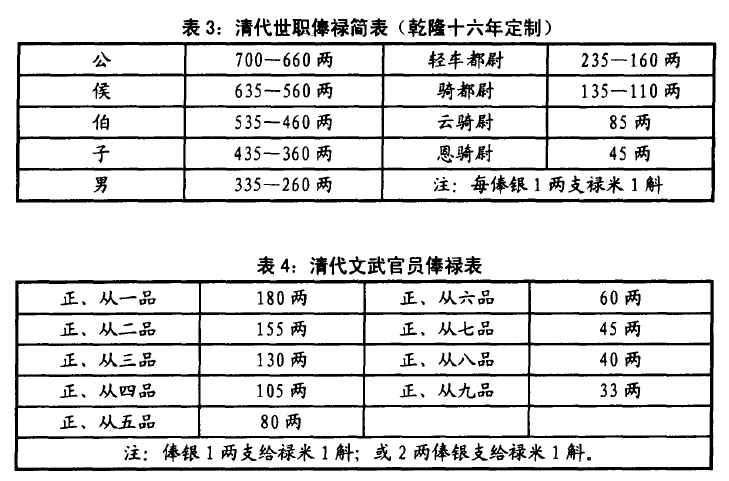
\includegraphics[width=0.5\linewidth]{images/fenglu.png}
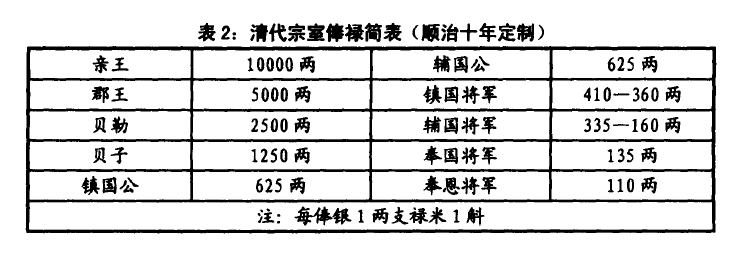
\includegraphics[width=0.5\linewidth]{images/fenglu2.png}
\end{figure}

曹雪芹进步妇女观的形成,既受明中叶以来的时代进步思潮影响,更与满族社会特殊的妇女地位有关。 

相对而言,清代八旗世家对封建礼法的恪守远甚于当时的汉族世家。 

旗人社会中的女子持家、重小姑、重内亲等习俗在《红楼梦》中都有生动体现

清代的满族贵族文化,是中国历史上在官僚社会中唯一形成了自己特色的贵族文化。 
“有闲性”是京旗文化的显著特征,并构成了与中国历史上影响深远的士文化的重要区别。 

最早的《三国志演义》还是半文半白,《水浒传》、《金瓶梅》使用的是山东方言,《西游记》、《儒林外史》用的则是长江流域官话,到《红楼梦》才真正开始使用北京话写作。 

《红楼梦》中不仅出现了“克什(恩赐)”、,'海龙(水獭)”、,'妞妞(女孩)“等满语词,而且满式汉语句俯拾即是,如“把莺儿不理”(第三十五回)、“何曾不是在房里来着”(第二十八回)、“将来只怕比这更奇怪的笑话儿还有呢”(第三回)、“要去不能”(第十九回)等,皆有满语语法的痕迹。 

内府包衣由于长期与满洲相处,潜移默化,姓氏逐渐满族化。姓氏满洲化是指放弃自己的汉族姓氏,随同满洲姓氏的特点,即”称名不举姓,人则以其名之第一字称之,若姓然“。

《红楼梦》成书时的传播路径: 
\begin{figure}[htpb]
\centering
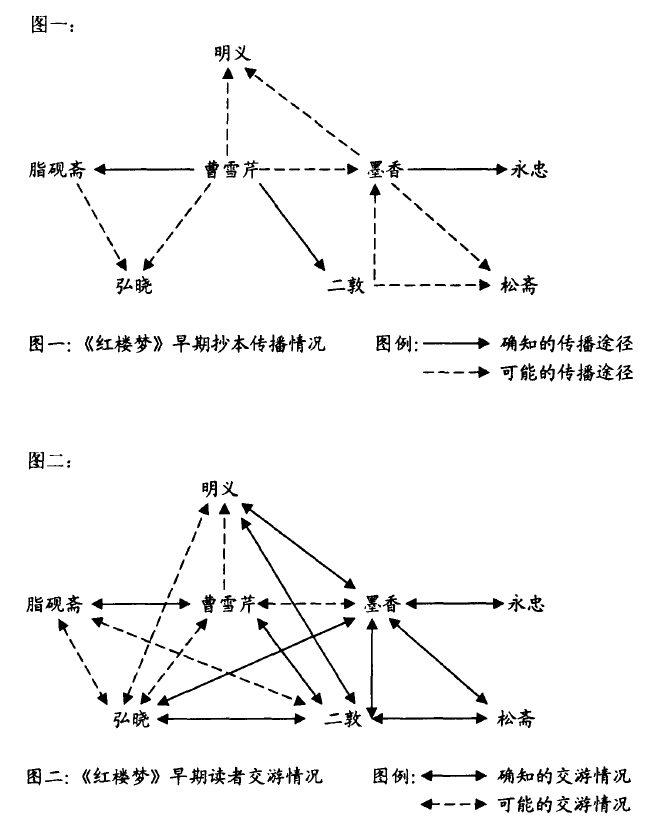
\includegraphics[width=0.5\linewidth]{images/hlmlc.png}
\end{figure}
\subsection{《月亮和六便士》}
\subsubsection{一些标注}
“女人可以原谅男人对她的伤害,”他说,“但是永远不能原谅他对她做出的牺牲。”

人们动不动就谈美,实际上对这个词并不理解;这个词已经使用得太滥,失去了原有的力量;因为成千上万的琐屑事物都分享了“美”的称号,这个词已经被剥夺掉它的崇高的含义了。一件衣服,一只狗,一篇布道词,什么东西人们都用“美”来形容,当他们面对面地遇到真正的美时,反而认不出它来了。他们用以遮饰自己毫无价值的思想的虚假夸大使他们的感受力变得迟钝不堪。正如一个假内行有时也会感觉到自己是在无中生有地伪造某件器物的精神价值一样,人们已经失掉了他们用之过滥的赏识能力。

她只差一点儿就称得起是个美人,但是正因为差这一点儿,却连漂亮也算不上了。

女人们总是喜欢在她们所爱的人临终前表现得宽宏大量,她们的这种偏好叫我实在难以忍受。有时候我甚至觉得她们不愿意男人寿命太长,就是怕把演出这幕好戏的机会拖得太晚。

在我同他打交道的时候,正是这一点使我狼狈不堪。有人也说他不在乎别人对他的看法,但这多半是自欺欺人。一般说来,他们能够自行其是是因为相信别人都看不出来他们的怪异的想法;最甚者也是因为有几个近邻知交表示支持,才敢违背大多数人的意见行事。如果一个人违反传统实际上是他这一阶层人的常规,那他在世人面前作出违反传统的事倒也不困难。相反地,他还会为此洋洋自得。他既可以标榜自己的勇气又不致冒什么风险。但是我总觉得事事要邀获别人批准,或许是文明人类最根深蒂固的一种天性。一个标新立异的女人一旦冒犯了礼规,招致了唇枪舌剑的物议,再没有谁会象她那样飞快地跑去寻找尊严体面的庇护了。那些告诉我他们毫不在乎别人对他们的看法的人,我是绝不相信的。这只不过是一种无知的虚张声势。他们的意思是:他们相信别人根本不会发现自己的微疵小瑕,因此更不怕别人对这些小过失加以谴责了。

“女人的脑子太可怜了!爱情。她们就知道爱情。她们认为如果男人离开了她们就是因为又有了新宠。

那时候我还不懂女人的一种无法摆脱的恶习——热衷于同任何一个愿意倾听的人讨论自己的私事。
\subsubsection{读后感}
作者犹如一个热爱八卦而又极度腹黑的……嗯,八婆,整天不干事却往来于社交场合,打听人的隐私八卦,面露和色却内心翻腾,让人讨厌。
\subsection{《素女经》}
\subsubsection{作者冯唐}

不停的贫,贫,贫,抓一些冷僻知识(其实不算多冷僻,百度百科上很容易找到,所以只能说是抖机灵,不算是卖弄),反复地讲道理说感想。

故事本身很简单:黄冈学霸清华毕业生斯坦福出身的田小明,在美帝遇见读研的师妹白白露,两人搞在一起。田小明受发小王大力邀请回国创业,创办生物高科技公司,遇见合作的咨询公司的万美玉,出轨也搞在一起,两人身体契合,心灵也契合。后来白白露发觉,也怀孕,万美玉也让田小明二选一,田小明暂时选择婚姻,半年后又出轨找万美玉,因为受不了后者的控制欲,跳楼坠亡,灵魂出窍又还魂,送进精神病院,出来后去西藏成了神迹一样的人物(这段无意有意在恶心西藏)。

这本书是黄书,性描写露骨,虽不算多出彩多优秀,但结合在情节里也算水到渠成,没有多刻意。但人物形象模糊,除了话唠外难以让人记清楚(有这种特点的小说,人物往往沦为作者观点的传声筒)。

作者常有妙语,可供消遣,如:
\begin{quotation}
像坏人的红酒就是好酒,一时让人开心,过后一直伤心。像小坏蛋的就是挺好的红酒,像大坏蛋的就是超好的红酒。
\end{quotation}

\subsubsection{田小明}
清华和斯坦福高材生,文理兼通,喜爱自摸和A片,更喜欢美女。讲话把生殖器和吹牛逼挂在嘴边,有趣,但不深刻;嘴欠,但说不上油滑;坦诚,但遮遮掩掩做不到完全的赤裸相见;还算专情,但责任感让位于生物本能和一时痛快。田小明懂女人,会搞女人,但丝毫不专一,并且毫不愧疚(或者毫不要脸)地把这归咎于生物本能。活的敞亮,但很猥琐,有高富帅的面目,但处处都为满足屌丝意淫的幻想(或许仅仅是作者冯唐的幻想)。

\subsubsection{白白露}
郑州人,清华大学电子系毕业,爱运动,长的漂亮但肯定不惊艳。似乎对男人本性放的很开,和田小明两地分居还叮嘱他可以嫖娼但不能有外遇(女人特殊的洁癖和贞操观)。分居久了田小明不再陪她也陪不了他就不再联系,但偷偷设置监控,监督田小明的一言一行,发现他把女人往家里带,回国生孩子,试图把田小明拉回自己身边,但田小明还是偷偷去找万美玉。

作者似乎很爱定义理工和文科学生的思维差别,也爱用清华和北大学生的梗。白白露作为清华理科女,具有所谓的“理科思维”,会搞硬件也会写程序,还会装监控搞偷窥。回国前白白露很大度,之后成了小家子气的女人,滑向心胸狭窄和控制狂魔的深渊。

\subsubsection{万美玉}
工作狂,条理分明,田小明身体和心理的红颜知己,“不顾一切”地和田小明约炮,试图让田小明脱离婚姻。在控制欲这一点上,和白白露如出一辙。
\subsection{《羊毛战记》}

\subsubsection{情节}
无非是个反乌托邦故事,不算是科幻(算不算蒸汽朋克?)。

未来的美国人生活在50个地堡里,
\begin{quotation}
整个地堡分为三段楼层,每一段四十八楼
\end{quotation}
里面有农业区、工业区,有保安官,有首长,但最核心的是有一个资讯区,他们有三层楼的空间,有很多服务器,用来保存内部历史信息。奇怪的是人们通讯大多通过邮差来上下楼梯送信,而不是电子邮件。电子邮件太贵,其目的也是为了不让人喜欢通信。

地堡有个奇怪的规定:不允许人们出去,谁一旦有了这种想法,当局立刻将其判处死刑,并拉出去清洗镜头。外面的世界是荒漠和海市蜃楼一般的城市,但城市都是断壁颓垣。出去擦镜头的人都需要穿上厚厚的防护衣,头盔里有一个显示屏可以“看到”外部影像(当然,影像是合成的“春意盎然”的假象)。他们需要使用“羊毛”来擦洗镜头。这些人每天在地堡里看到外部的影像是荒凉的(但却是真实的),而在头盔里看到的却是有生机的,因此他们乖乖擦完镜头后立刻迫不及待想到翻过镜头看不到的山丘去生机勃勃的城市。但资讯区的人在防护衣上做了手脚,密封胶带是劣质的,很容易漏气,因此这些人没走几步都会因吸入毒气而死去。

对此人们当然不会坐视不管,
\begin{quotation}
平均大概每隔二十年就会有一次大规模的暴动。
\end{quotation}
但每次暴动之后资讯区的人都会删除所有历史资料,因此后来的人们难以获知这些秘密。

地堡之间会通过资讯区的头头之间联络,以获悉哪些地堡会废弃。资讯区头头会有一个秘密房间,这个房间有所有人类以前的历史和五十个地堡的地理位置。地堡实施学徒制,资讯区头头也会到一定时间选择一个“可靠”的人来做学徒(竟然不实行我党的历史审查和档案制度,真是二!),并把一本“地堡运行指南”让他读,
\begin{quotation}
有好几个章节是在解释什么叫作“说服群众”,什么叫作“思想控制”,什么叫作“恐吓式教养的效果”,另外还有一大堆关于人口控制的图表……
\end{quotation}
(从上文就可以看出来作者根本就对共产党和极权主义缺乏了解,这些手段相对于真实的历史真是小儿科,根本就不管用。好好看看苏联和我党历史吧少年!)

地堡竟然实施选举制而非威权和极权体制,这让我很惊讶。这快死了还搞个啥民主?正如作者所说,
\begin{quotation}
“如果你不想失去孩子,那你就必须对他们残酷一点。”
\end{quotation}
所以搞点血腥政治,搞点互相检举揭发啥的很必要啊!

第一章霍斯顿夫妻俩前仆后继出去擦镜头的情节很好看,紧凑合理,扣人心弦。

第二章里詹丝的心理活动就差远了,很难想象这种随波逐流缺乏干练和决断力的思考会来自一个首长,会来自一个老年人。这让人觉得,地堡并不需要一个首长,她就像是一个橡皮图章,缺乏一个领导人应该有的那种权威和大权在握。

自从茱丽叶被送出去之后,这部小说对读者就没有什么秘密了,完全成了拖沓的拼凑故事。

茱丽叶和卢卡斯的生死之恋莫名其妙。

暴动就是走过场,没啥亮点。

十七号地堡里的故事也很乏味。

整个故事架构构造还不错,前期故事很有张力,但bug太多,无法解释。

坑爹的小说,只配两星。据说是美国去年销量很高的小说,对此我只能说,读书一定要远离所谓畅销书。

\subsubsection{白瑞德}
为什么单说这个人?这个人的行为完全反映了作者坑爹的人设。卢卡斯被任命为学徒(其实就是指定接班人)前,这个人的形象完全是反面的狰狞的,害死茱利叶前男友、害死詹丝、强势夺权、试图害死茱利叶等等和后面的反转虽说不上突兀,但反派突然正面化就使全书缺乏一个刺激的愿景,读者开始无所适从。白瑞德对卢卡斯谆谆教导颇有长者风范,系万民生死于一身让充满好感,但手下反水放茱利叶十八号地堡立刻被压权,丝毫没有反手之力,虎头蛇尾。

\subsubsection{茱利叶}
主角身上有强烈的光环,鬼挡杀鬼佛挡杀佛,大难不死,福寿安康。作者一介绍茱利叶,特别是詹丝一死,读者立刻会知道茱利叶才主角,肯定死不了(KINDKE的X-RAY里能看出来)。茱利叶能修发电机能修机器,能潜水,意志力坚强,体力旺盛,都不像个女人。

坑爹的是茱利叶卢卡斯间的爱情,看了一次星星突然就发生了,用电话聊了几次天突然就成生死至交了,茱利叶一回十八号地堡几乎就要结婚生子了。前景铺垫太少,后面就太突兀。

\subsubsection{卢卡斯}
这人没能力没皮相没魄力,却突然被指定为地堡实际的继承人,突然让白富美茱利叶一见倾心抱得美人归,突然就策动政变端掉了自己老板,名利双收,比主角的光环都亮。

\subsubsection{老沃克}
毫无性格,在机电部却会折腾无线电,竟然能听到别的地堡的信号。隐忍多年救下出去擦镜头的茱利叶,按说挺有智慧,眼睁睁看着机电区的人出去暴动(送死)。
\subsection{《长恨歌》}

\subsubsection{王安忆}

王安忆的文字在这篇小说里琐碎絮叨,写一个上海女人如何从少女时代到死亡的生活细节和心态演变,“说不尽的愁肠百转”。王安忆笔下有烟火气,是过日子把所有的激情和棱角都磨平再泡软的心态。

第一部里李主任程先生的情节已经写得很好,第二部里邬桥里轻轻一转,到了严家师母和毛毛娘舅,又是打牌又是算命,又是吃鸭又是比美,恍若隔世的感觉,翻出新情节,赞叹作者的笔力绵长沉稳。然而,王琦瑶自从死了金主,便如同死了自己,再也提不起生活的乐趣,也无法再爱上哪个男人。她的后半生(其实是从18岁以后),便如同寡妇一般,失去了所有的鲜美颜色和激情,只剩下过去的回忆和狼藉的内心。一个女人的一生,基本被年轻的小三生活给毁掉了(警醒啊女同志们!)。

这篇小说写女人,在我看来比绝大多数男作家要好得多。刘慈欣阿西莫夫这样的就不说了,他们写女人和写男人完全没有分别,性别在他们笔下根本无从展现;即使是金庸这样的专业作家,笔下的女人虽说“千种风情”,但给人感觉还是如出一端,都是作家自己的意淫和捏抟;曹雪芹写女人当然基本上已经是最好的文笔了,但还是有男作家的影子。只有女性作家自己体会自己观察,才能把女人写好。在这一点上,最起码,王安忆做到了。

王琦瑶和蒋丽莉、吴佩珍间的友情或“闺蜜”情,在我这种直男癌或外人看来似乎十分亲密并且掏心掏肺,但在作者笔下却是一种暗暗战争暗暗较劲甚至“阳奉阴违”的过程。女人心海底针,三个女人一台戏,不是没有道理的。女人心里的那种小九九,让男人去写完全不行,非得王安忆这种女作用才能写出来。其实这种东西,虽然称不上深刻高尚,但写下来仍旧很耐看。特别是王安忆擅长写人物的感觉,擅长用一些简短的比喻来修饰人心的描画,这种琐碎的不厌其烦的描写往往也比较耐看。

女人柔情,女人琐碎,女人“没见识”,女人爱时尚爱衣服,女人“小心眼”。闺蜜之间是这样的:
\begin{quotation}
她们的做伴,其实是寂寞加寂寞,无奈加无奈,彼此谁也帮不上谁的忙,因此,倒也抽去了功利心,变得很纯粹了。
\end{quotation}
她们见多了繁华,因此要“过好日子”,苦日子她们应该是受不来的,她们见过爱情,也见过婚姻,但似乎都没有那些流动的繁华和万人瞩目更让人倾心,
\begin{quotation}
两人又默默地走了一段,王琦瑶缓缓地劝慰说:其实再怎么样,也还是结发夫妻最恩深义长。严家师母笑了,点着头道:是啊,有恩有义是不错,可你知道恩和义是什么吗?恩和义就是受苦受罪,情和爱才是快活,恩和义是共患难的,情和爱是同享福的,你说你要哪样?
\end{quotation}
女人和女人混在一起,彼此相距很近,她们的内心却未必近,
\begin{quotation}
好在女人和女人是不怕种下芥蒂的,女人间的友谊其实是用芥蒂结成的,越是有芥蒂,友情越是深。她们两人有时是不欢而散,可下一日又聚在了一处,比上一日更知心。
\end{quotation}
王琦瑶和严家师母间“比美”的心态,很值得玩味,很细腻,男性作家写不出:
\begin{quotation}
自从烫了头发,王琦瑶又有了些做人的兴趣了,从箱底翻出旧日的好衣服,稍做修改便是新。她也开始化妆,修眉毛的钳子、眉笔、粉扑都还在,一件件找出来摆开。她在镜子前流连的时间多了些,镜子里的人是老朋友,也是新认识,能与她说话的。严家师母看见她的变化,暗中加了把劲追赶。王琦瑶显见得比她懂打扮,也是仗着年轻有自信,样样方面都是往里收,留有余地,不像严家师母是向外扩张,非做到十二分不可。一个是含而不露,一个是虚张声势;一个是从容不迫,一个是剑拔弩张。严家师母不使劲还好,越使劲越失分寸,总是过火。王琦瑶当然觉察出严家师母的用力,更上了几分心。像她这样的聪敏,不上心就是合适,再要上心便是格外好了,由不得严家师母不服气。有几次,她甚至是忍了泪的,回到家中无由地向娘姨发脾气,还把新做的头梳乱,自己报复自己的。但脾气发过了,还是重整旗鼓,再与王琦瑶较量。这几日,严家师母到王琦瑶家,不是为别的,专是挑战而来的。她越这样,王琦瑶越不让她,每天都给她个出奇制胜,并且轻而易举,不留痕迹。严家师母话里面就有几分酸意了,说王琦瑶真是可惜了,这般的浓妆淡抹也相宜却无人赏识。王琦瑶知道她是发急,嘴里说的未必是心里想的,听了也当没听见,只是下一回再用些心,更上一层楼,叫她望尘莫及。这两个人勾心斗角的,其实不必硬往一起凑,不合则散罢了。可越是不合却越要聚,就像是把敌人当朋友,一天都不能不见。
\end{quotation}
相比之下,似乎男人之间的距离就大多了。所以,家里需要有一个女人,没有女人,似乎就不是过日子,
\begin{quotation}
家里有两个女人,再没个男人来解围,事情是真难办。倘要以为这个没有父亲的家庭会受到种种压力,那也大错特错了。
\end{quotation}

\subsubsection{上海}

王安忆写上海几十年的变迁,不仅从人物身上,从事件身上,也从潮流时尚(穿衣、跳舞、电影)上,从人情和生活琐碎上。上海的弄堂里有鸽子,它们眼看着上海几十年的恩怨,看王琦瑶沉沉浮浮。上海的弄堂里有爬山虎,有洗衣服和晒衣服的气味,这一点上王安忆把握得很细致(虽然未必称得上是精准,不是上海人我无法判断)。

上海在王安忆笔下,繁华里带着落寞,气派里带着小家子气,温柔里带着勾心斗角。上海人是势利的,是小市民的(所谓“小家碧玉”无非就是小市民);上海的繁华是权力和财富带来的,是外人(外国人和外地有钱或有权的人)带来的,因此上海人是倚势的。他们称呼人是“瘪三”,称呼人是“乡下人”,似乎自己高人一等。王安忆一针见血(却温柔)地说:
\begin{quotation}
这城市里的真心,却惟有到流言里去找的。\emph{无论这城市的外表有多华美,心却是一颗粗鄙的心},那心是寄在流言里的,流言是寄在上海的弄堂里的。这东方巴黎遍布远东的神奇传说,剥开壳看,其实就是流言的心子。
\end{quotation}
上海是如何变成上海的呢?
\begin{quotation}
由于人口繁多,变化也繁多,这城市一百年里积累的隐私比其他地方一千年的还多。
\end{quotation}
与其说是繁华,不如说是浮华,这种繁华只是场面,见惯了风月场,见多了金钱,但生活还是生活,这种“见识”离生活有点远,于是人就不“踏实”了,就眼看着远方却不看脚下了,
\begin{quotation}
街上走的人,都是戴了假面具的人,开露天派对的人,笑是应酬的笑,言语是应酬的言语,连俗套都称不上,是俗套外面的壳子。
\end{quotation}
上海的女人美丽,有见地(看看王琦瑶、张永红、康明逊等人对生活精细和穿衣时尚的重视和追求有多强烈!),但这种见地仍然只是小家子气的,是要通过和人比较的,不是自我的信心,而是来自他人的羡慕的眼光,
\begin{quotation}
上海的小姐们就是与众不同,她们和她们的父兄一样,渴望出人头地,有着名利心,而且行动积极,不是光说不做的。她们甚至还更勇敢,更坚忍,不怕失败和打击。上海这城市的繁华起码有一半是靠了她们的名利心,倘若没有这名利心,这城市有一半以上的店铺是要倒闭的。上海的繁华其实是女性风采的,风里传来的是女用的香水味,橱窗里的陈列,女装比男装多。那法国梧桐的树影是女性化的,院子里夹竹桃丁香花,也是女性的象征。梅雨季节潮黏的风,是女人在撒小性子,即唧哝哝的沪语,也是专供女人说体己话的。这城市本身就像是个大女人似的,羽衣霓裳,天空撒金撒银,五彩云是飞上天的女人的衣袂。 
淮海路的女孩还是有些野心的,她们目睹这城市的最豪华,却身居中流人家,自然是有些不服,无疑要做争取的。
\end{quotation}
上海并非孤悬海外。上海人也是南方人,特别是苏州人(上海与苏州的关系,有待好好探求),
\begin{quotation}
苏州是上海的回忆,上海要就是不忆,一忆就忆到苏州。上海人要是梦回,就是回苏州。甜糯的苏州话,是给上海诉说爱的,连恨都能说成爱,点石成金似的。上海的园子,是从苏州搬过来的,藏一点闲情逸致。苏州是上海的旧情难忘。
\end{quotation}
上海的小市民们,似乎对政治不上心,这可能是远离政治中心的缘故,也可能是北京离他们太远的缘故,也可能北京带来的政治文化和手段(共产党是泥腿子进城,要打倒官僚资本主义和小资产阶级,不就是把旧上海的人和生活连根拔起嘛?)和他们的生活太遥远的缘故,
\begin{quotation}
(王琦瑶和程先生)和所有的上海市民一样,共产党在他们眼中,是有着高不可攀的印象。像他们这样亲受历史转变的人,不免会有前朝遗民的心情,自认是落后时代的人。他们又都是生活在社会的心子里的人,埋头于各自的柴米生计,对自己都谈不上什么看法,何况是对国家,对政权。也难怪他们眼界小,这城市像一架大机器,按机械的原理结构运转,只在它的细部,是有血有肉的质地,抓住它们人才有依傍,不致陷入抽象的虚空。所以,上海的市民,都是把人生往小处做的。对于政治,都是边缘人。你再对他们说,共产党是人民的政府,他们也还是敬而远之,是自卑自谦,也是有些妄自尊大,觉得他们才是城市的真正主人。
\end{quotation}
这一点和北京人几乎完全相反。北京人见多了权力,见多了兴亡,对这种天子威严很有爱好,以此作为骄傲。

看看程先生,再看看李主任,他们对待女人的做法完全不同,得到的结果也完全不同。李主任有权力,经历的女人多,知道女人的胃口喜好,所以游刃有余如烹小鲜。这是实力,没这实力就表现不出这种自信,只能强撑场面。

\subsubsection{爱情}

对待女人,不应该周旋,应该强势侵入。周旋是女人的做派,女人生活在女人世界,唯一缺乏的就不是周旋。程先生不停周旋,只会让蒋丽莉和王琦瑶都不满意。女人需要的侵入,如同男根的侵入一样,是饱满的自信的,是雄伟的,是斩金截鉄的。女人只需要说 yes 或 no,不需要费尽心机去选择去做决定(美其名曰“你要对我负责”)。这样的侵入不是贫穷和委顿能带来的,只能从充沛的体力、雄厚的财富和志得意满的权力得来。

王琦瑶对程先生不上心,对李主任可谓情深义尽。从个人的角度上看,可以会觉得程先生是一个“好男人”,而李主任不过是个有钱有权有能力的大叔。但王琦瑶似乎缺乏一种父爱和稳固的安全感,对李主任的这种角色深深迷醉不能自拔,她的小聪明和“小”深情都献给了这位“宋思明”。

读到康逊明那段还好,再往下就是三观齐毁道德败坏自作自受了。自己的孩子却给别人戴绿帽,自己不负责任,婆婆妈妈不当机立断,害人害己,真想来一句活该。不过,王琦瑶和康逊明挑明感情那段写得真好。

\subsubsection{王琦瑶}

不喜欢这种女人:殊无才华,身无长物,追逐时尚潮流,依靠男人,却又目下无尘,过不得日子。

不过首先来说,王琦瑶是个美女,
\begin{quotation}
王琦瑶的美不是那种文艺性的美,她的美是有些家常的,是在客堂间里供自己人欣赏的,是过日子的情调。她不是兴风作浪的美,是拘泥不开的美。她的美里缺少点诗意,却是忠诚老实的。她的美不是戏剧性的,而是生活化,是走在马路上有人注目,照相馆橱窗里的美。从开麦拉里看起来,便过于平淡了。
\end{quotation}
出道前的王琦瑶有着少女的羞涩与拘谨,甚至是呆板,不灵动,但选美让她潜在的美都绽放开来,
\begin{quotation}
一笑,表情舒展了,脂粉的颜色里有了活气,便生动起来。再看那镜子里的美人,也不那么生分和隔膜了。
\end{quotation}
其实这种美,是深得男人喜爱的。男人自然各种口味都有,也常常换口味,但对这种美女,大概绝大部分男人的绝大部分时间里,是不会拒绝的。这或许能解释,为什么王琦瑶这个多年在男人心中长盛不衰的原因,为什么她身边总不缺少爱慕者的原因。

王琦瑶的一生都被突如其来的恩宠荣耀给毁了,被当小三的轰轰烈烈给毁了,被顾影自怜和自作自受给毁了,被绿茶婊的内心和眼高手低给毁了。年轻之后的种种悲惨遭遇都和当时的选择不无关系。其实她的生活,本来可以平衡如湖水,但非要渴望大风大浪,因为虚荣心,拿自己的美貌玩了一次野心,
\begin{quotation}
(为了选美)王琦瑶其实是真正地起了奢望。她的心本来是高的,只是受了现实的限制,她不得不时时泼自己的冷水。她知道这世界上的东西真是太多了,越想要越不得,不如握牢自己手中的那一点,有一点是一点,说不定反会有意外的获得,所以是越不想越能得。
\end{quotation}
大体上讲,王琦瑶是小家碧玉,不是大家闺秀,有小家碧玉的野心,有小家碧玉的精明和择木而栖的圆滑,见过大阵仗,有上流社会的经验却不能时时过上上流生活,有知识文化,其实本质上也算独立,但就是会自视太高给自己找罪受。

看看王琦瑶被李主任包养前的这段心理,好好的干吗干这行?可是,在她们眼里,女人只有依附权力,依附财富,依附男人,才能光鲜亮丽,才能让她们内心有希望:
\begin{quotation}
望了一溜烟而去的汽车,王琦瑶是有点怅惘的。李主任说来就来,说去就去,来去都不由己,只由他的。明知这样,还要去期待什么,且又是没有信心的期待,彻底的被动。以后的几天里,李主任都没有消息,此人就像没有过似的,可那枚嵌宝石戒指却是千真万确,天天在手上的。王琦瑶不是想他,他也不是由人想的,王琦瑶却是被他攫住了,他说怎么怎么,他说不怎么就不怎么。这些日子里,王琦瑶成天地不出门,程先生也拒绝见的。倒不是有心回避,只是想一个人清净。清净的时候,是有李主任的面影浮起,是模糊的面影,低着头用眼里的余光看过去的。王琦瑶也不是爱他,李主任本不是接受人的爱,他接受人的命运。他将人的命运拿过去,一给予不同的负责。王琦瑶要的就是这个负责。这几日,家里人待王琦瑶都是有几分小心的,想问又不好问。李主任的汽车牌号在上海滩都是有名的,几次进出弄堂,早已引起议论纷纷。王琦瑶的闭门不出也是为了这个。
\end{quotation}

\subsubsection{程先生}

婊子自有备胎磨。程先生大体算是文艺青年,偏偏看上小家碧玉的王琦瑶。推想一下,程先生条件不差,跟王琦瑶算是一个档次的,郎才女貌,品性眼光都很配。程先生当然看不上蒋丽莉那样莽撞的没有涵养的女生,但真正的豪门千金大家闺秀他又吃不起。王琦瑶是程先生层次上最好的选择,爱上王琦瑶对他而言一点不意外。

程先生相对于毛毛娘舅,相对于萨沙,还是比较有担当的,但这种所谓担当无非是做一个接盘侠来暂时照料怀孕和生产中的女神,他并没有“非分之想”,没有勇气跨出这一步。这真是屌丝的悲哀!在屌丝眼里,女神圣洁不可侵犯,不把自己的占有欲望当回事,错失良机。

值得玩味的是,正如大多数屌丝一样,程先生付出,接近,自己被自己感动得稀里哗啦,
\begin{quotation}
他站在她的身后,嗫嚅了一会儿,说道:伯母,请你放心,我会对她照顾的。说完这话,他觉着自己也要流泪,赶紧拎起热水瓶回房间去了。
\end{quotation}
你说你有啥好哭的?直接推倒过日子不就得了?

程先生敏感、纤弱,不敢得到却常常怅然于失去(其实什么也没有失去),
\begin{quotation}
程先生的两次恋爱都是折磨人的,付出去的全是真心,真心和真心是有不同,有的是爱,有的是情义,可用心都是良苦,然而收回的是什么呢?因此,他开始从根本上怀疑有没有什么两情相悦。他想男女之情真是种瓜不得瓜,种豆不得豆。不得是磨人,得也是磨人。
\end{quotation}
最终程先生在文革开始里自杀了。程先生这种人,根本就缺乏生存的活力和欲望,不能在这种残酷的条件下生活。即使不是因为王琦瑶,他这种人也活不长久。

\subsubsection{康明逊(毛毛娘舅)}

此君生母是个小,把大母当亲妈,见过新生母亲无人可言的凄凉,就产生自怜和自暴自弃的情绪。另外,他也缺少担当(除了李主任,这部小说哪个男人有担当?这些男人啊,细腻倒是细腻,知心倒是知心,但就是缺少一股子男性气概),自己有了女儿却不敢认。王琦瑶也是“活该”碰到这种人。
\subsection{《百年孤独》}
\subsubsection{标注}
正象神父所预言的,从此没有一个新娘不身怀怪胎,炎热也始终不见减退。

在那么多年没有生儿育女的同居之后,他俩在热恋中奇迹般地欣然发现,餐桌边的相爱比床上的相爱毫不逊色。他们感到了这样一种幸福:虽然精力衰竭,上了年纪,却依然能象家兔那样嬉戏,象家犬那样逗闹。

“你生下蜥蜴,咱们就抚养蜥蜴,”他说。“可是村里再也不会有人由于你的过错而被杀死了。” 这是一个美妙的六月的夜晚,月光皎洁,凉爽宜人。他俩通古未睡,在床上折腾,根本没去理会穿过卧室的轻风,风儿带来了普鲁登希奥·阿吉廖尔亲人的哭声。
\subsection{《银河帝国》}
\subsubsection{主要情节}
\paragraph{基地三部曲}

\paragraph{基地前传}

\paragraph{机器人五部曲}

\paragraph{外篇:我,机器人}

\paragraph{钢穴}

\paragraph{裸阳}

贝莱奉命到索拉利星侦破机器人杀人案,遇到死者妻子嘉蒂亚,……

\paragraph{曙光中的机器人}

贝莱奉命到奥罗拉星侦办人形机器人詹姆斯停摆案件,被告为其设计者法斯陀夫博士,因为只有他才有足够的知识让人形机器人停摆。嘉蒂亚来来到奥罗拉后和法斯陀夫博士是邻居,詹姆斯是服侍她的,她把詹姆斯当成“性伴侣”。同时,法斯陀夫博士的对头——阿玛狄洛的指使人使詹姆斯停摆,试图借此攻击法斯陀夫(只有法斯陀夫有能力去做这种事情)。阿玛狄洛试图消灭贝莱,但后者借助机器人丹尼尔和吉斯卡的力量挫败了前者的阴谋。

吉斯卡具有重要的能力:看透人的心灵并在一定程度上改变人的想法。

\paragraph{机器人与帝国}

两百多年后,地球在贝莱和法斯陀夫的合力下开始向外太空移民,这些人称为“银河殖民者”。银河殖民者控制了很多星球,这给了太空族很大压力,奥罗拉上的阿玛狄洛试图在地球上建立基地,改变地球内部的放射性,从而逐渐使地球成为一个“死星”,借此消灭地球人和太空殖民者。但丹尼尔和吉斯卡通过控制形势和人的心理,挫败了他们的阴谋。

在这个过程里,丹尼尔悟到了“第零法则”,认为机器人应当对人类整体负责,最后吉斯卡停摆前将自己的能力给了丹尼尔。

\subsubsection{一些标注:}
我绝不要出卖我的独立性,以换取某种短暂的快感。”

“如果没有一群异于凡夫俗子的人,就不可能出现天才和圣者,而我不信异于常人的人都集中在好的一端,我认为一定有某种对称存在。

一个孤立体——孤立的个体——可能会说谎,因为他是有限的,所以他会感到恐惧。然而,盖娅是个具有强大心灵力量的行星级生命体,根本就没什么好怕的,因此盖娅完全不需要说谎,或是杜撰一些与事实不符的陈述。”

关于银河帝国三种走向的表述:
\begin{itemize*}
	\item “以川陀为蓝本所建立的第二银河帝国,将是一个父权式帝国,依靠算计建立,依靠算计维持,在无尽的算计中,它永远是行尸走肉。那会是个死胡同
	\item 以端点星为蓝本所建立的第二银河帝国,将是一个军事帝国,依靠武力建立,依靠武力维持,最后终将被武力摧毁。它会是第一银河帝国不折不扣的翻版,
\end{itemize*}
银河中搞不好有百万种智慧生物,却只有一种是扩张主义者,那就是我们。其他的都安分守己地待在母星,隐藏起来……”

理论上,基地公民人人平等,可是出身于联邦原始成员的公民,却比其他世界的人更平等些。至于那些跟联邦之外的世界有渊源的人,则是所有的公民中最不平等的。

双手才是真正的工作界面,

假如第二基地确实存在,却又希望保住这个秘密,那么有一点是绝对肯定的。如果有谁认为它仍旧存在,并且和他人讨论这个可能,甚至在公开场合高谈阔论,闹到整个银河人尽皆知,那么他们一定会立刻用巧妙的手法,将这个人解决掉、铲除掉、消灭掉。

(第二基地)他们的干预尽可能做得精巧、间接和分散。

“你所谓的‘超自然’是什么意思?” “最明显的意思──相信某些实体独立于自然律之外,比如说不受能量守恒或作用量常数的限制。”

历史在在显示,我们无法从历史中学到任何教训。

(地球人和从地球出发的太空殖民者)我们共有三项优势:因为没有机器人,我们用自己的双手打造新世界;因为世代交替迅速,我们一直在求新求变;而最重要的是,地球这颗母星是我们的中心信仰。”

多半要归咎机器人!它们降低了人类的互赖性,填充了人与人之间的空隙。人类彼此间原本存在着自然的吸引力,机器人却将它阻绝,于是整个社会崩解成了一片散沙。

有可能群众人数越多,就越容易受到情感而非理智的影响。

群众显然要比个人容易操纵。

每一个被我强化的心灵,都会再强化附近另一个同质的心灵,接着周遭又会有更多的心灵受到它们的强化。

(奥罗拉的科学)在一个长寿的社会中,压力相对小得多。我们的科学家能用三到三个半世纪的时间,专心研究一个问题,因此逐渐有人认为,自己即使单打独斗,也有机会得到重大的进展。久而久之,就滋生出一种学术性的贪婪——想要自己独力完成某项研究,将科学进展的某个方面视为私产,宁愿眼睁睁看着整体发展慢下来,也不愿舍弃自己心目中的禁脔。结果,太空族世界的整体科学发展就真的变慢了,甚至到了难以超越地球的地步,虽说我们掌握了极大的优势。”

厄俄斯是古希腊的曙光女神,正如奥罗拉是古罗马的曙光女神。”

别人的哀痛总是容易被讲成人生哲理。”

退化”或许就该这么定义:让人很容易适应的事物。

机器人的尸体竟然比人类尸体更像人类,

而我们脚下的这座厄俄斯城,正是这个世界的行政中心。总共有两万人住在这里,因此不只奥罗拉,就算在整个太空族世界,它也是最大的城市。要知道,整个索拉利的人口加起来也只有那么多。”

(奥罗拉)它一天只有22个小时。” “应该说是22.3个传统小时。每个奥罗拉日有10个奥罗拉时,每个奥罗拉时有100个奥罗拉分,每个奥罗拉分又有100个奥罗拉秒。因此,一个奥罗拉秒大约等于0.8个地球秒。”

在一个接受机械劳工的经济体系中,机器人对人类的比例一律会直线上升,任何试图避免这个趋势的法规命令都是徒劳的。上升的速度虽然缓慢,可是永远不会停止。起初人口会显著增加,但机器人增加的速度却快得多。

对机器人下一个简单的命令,看着他乖乖服从,等于在强调自己是人类,而他只是机器人。

有些事物甚至凌驾于你脑中的那组正义之上。人类内心有一种冲动叫做慈悲,化为外在的行动则称为宽恕。”

有待测试的功能越重要、越基本,所需要的设备就越简单。这个道理同样适用于机器人,

(机器人的理解)“所谓的正义,以利亚,就是让所有的法律都发挥应有的效力。”

凡是在公家机关讨生活,个人能力永远比不上交际手腕来得重要,

我无法接受“如果知识代表危险,无知就是解决之道”这样的观点。在我看来,解决之道似乎是善用人类的智慧才对。人类不该拒绝面对危险,而应当学习如何化险为夷。

\subsubsection{一些感想:}
《银河帝国》里的计谋和政治实在是幼稚到家了,简直就是小孩子过家家的水平!另外叙事太直线化,人物太扁平化。阿西莫夫的文采太差了,比刘慈欣还要差,大刘最起码景物描写一笔带过却常常有传神之笔,阿西莫夫却只是干巴巴的叙事。

基地系列写作时间太早,到了机器人系列,阿西莫夫的文笔有了长足进步,以利亚·贝莱的形象就比哈里·谢顿丰满得多,也自洽得多。情节上,机器人五部曲更像是悬疑推理小说,读者的沉浸感会更强烈。

阿西莫夫在漫长的写作生涯中,应该是不断尝试新的技巧和手法的。阿西莫夫的特点在于喜爱通过人物对话来推动情节,优点是显得比较自然(只是相对显得),缺点是人物对话非常多,对人物和社会的情境反映太少,而后者正是科幻小说的魅力所在。科幻小说是生生造出一个世界,一个和现在不同的世界,仅仅通过人物的对话,对社会整体的反映实在太少。 

阿西莫夫在前期作品中对女人以及成人内容描述很少,似乎有读者对他反映,他也承认了这一点,于是在《裸阳》中出现了嘉蒂亚的裸体和男女接触的心理,出现了男女SEX造人的描述,到了《曙光中的机器人》更是把嘉蒂亚的性心理赤裸裸地描述出来,在《机器人与帝国》中她和以利亚甚至太空约炮。想想一个老头子对自己的不断“超越”,还是挺有意思的。

在太空族和地球人的争霸中,作者提到,太空族不受病菌感染,同时有机器人服务(灭菌并不必然导致长寿命,阿西莫夫明显并没有考虑人自身的疾病,比如免疫系统、细胞衰老等),寿命很长,因此社会发展滞后,缺少创新和冲劲。比如太空族的科研工作者都是各自为站,缺少交流,一个人研究出了人形机器人或看透心灵的机器人,别的研究院合多个之力仍然不能做出来。相反,地球人人口数量多,寿命短,因此有冲劲,创新能力强。我对这种社会学的判断持怀疑态度。
\subsection{《无声告白》}

\subsubsection{一些标注}
在这个夏天剩下的日子里,以及以后的很多年,詹姆斯和玛丽琳说话时会选择真正能表达自己的意思的措辞,无论是对内斯,对汉娜,还是互相之间。他们需要说的太多太多。

对逝去的心爱之人的记忆,会自动变得平顺和简单,它会把各种复杂纠结的成分当成丑陋的鳞片一样甩掉。

\subsubsection{读后感想}
玛丽琳无疑是这本小说的主人公。她的母亲无时无刻不希望她能成为一个典型的家庭主妇,每天为丈夫及孩子们烹饪出可口的饭菜。但是,母亲的强烈愿望受到了玛丽琳同样强烈的反判。她想“与众不同”,摆脱家庭主妇的命运。于是她在女子大学里选修了理科科目,并发誓就读医学院,成为一名医生,彻底走出母亲的阴影。然而,天真的她在没有任何计划的情况下和华人后裔詹姆斯坠入了爱河并很快结婚,虽然母亲在婚礼当日反对他们的结合。母亲的理由很简单:你们不一样。母亲没有说出口的是,他们是如此不一样,以致于在以后的生活里需要互相迁就的地方太多。然而,年轻的玛丽琳当然看不到这些,热恋中的她只看到“独一无二”的詹姆斯,看到他与众不同的那些闪光点,而这一直是她热切想得到的。但是,由于抚养孩子的压力,以及更重要的,社会对女性的偏见,使她不得不中断学业,在家相夫教子,成为自己最不想成为的家庭主妇。果然,对母亲的反叛,最终绕了一个圈,却过起了母亲那样的生活。但是这样的生活她是忍受不了的,那个”成为医生“的愿望是如此强烈,驱使她在已经有了两个孩子的情况下逃避到远方的社区大学去进行未完成的学业。然而,家庭的负担、对儿女的思念还是压过了她的个人理想,她不得不彻底向现实屈服,回到家里。但是,此时的她再也不会去用心烹饪,同时她把自己全部的未实现的愿望都毫无保留地转移给很像自己的女儿莉迪亚,以爱的名义”强迫“她好好学习,将来成为一名医生。她把莉迪亚的课程排得满满的,直接向那个最后目标冲刺,不给女儿丝毫的空间和自我意志。同时,对于其他孩子,比如大儿子内斯,以及小女儿汉娜(她和詹姆斯更忽视汉娜),他们几乎没有给予任何主动的关心,即使有,也是伴随着莉迪亚的。玛丽琳的这种失败母亲的做法,为家里的悲剧埋下了巨大的隐患,然而,在”实现自己理想“和”督促莉迪亚实现自己的理想“的道路上,她根本没有任何反省,对于母亲的生活方法,完全是一种玩命逃脱的姿态。

作为一个华人后裔,詹姆斯的父母只不过是飘洋过海的底层工人而已,种族的鸿沟使他敏感、自卑,渴望融入美国的”主流社会“,渴望获得白人的承认,渴望与人的交流。玛丽琳作为一个标准的”美国人“和”白人“,使他误以为通过爱情和婚姻就能将鸿沟填满,于是在玛丽琳天真的初吻后,他立刻接纳了她。但是,作者虽然没有明说,婚后的家庭里,凡事都是玛丽琳说了算的,他作为一个父亲却唯玛丽琳马首是瞻,在家庭里没有占据主导地位(美国家庭或许不如中国那样”传统“,但像詹姆斯这样把家事完全托付给玛丽琳的行为还是太”前卫“了一点)。她对儿女唯一的的教导就是拿自身缺乏的那些东西进行说教,希望他们能够”多交朋友“”融入社会“。当家庭里的重心渐渐被玛丽琳占据,他被排斥在儿女考育之外,只能三点一线,专注工作。在高校里,他遇见同样是华人后裔的路易莎,由于具有相同的文化背景,属于相同的种族,尤其是都能体会到少数族裔被主流社会有意无意排斥,他们越走越近,不过并未发生关系。当莉迪亚溺亡,玛丽琳歇斯底里的态度令他彻底对家庭失望,他无奈投入路易莎的怀抱。整篇小说里,詹姆斯很重要,但并非缺点,他似乎只是玛丽琳得以发现自己的一面镜子。

受到母亲”故意走失“的巨大刺激,莉迪亚对母爱的渴求非常强烈,她担心母亲再度”走失“离开自己,于是以答应母亲的所有要求来与母亲”交换“。在这种可悲的交换中,玛丽琳毫无所知,所有的伤害都被几个孩子默默承受。整个家庭由于母亲的偏执而无法进行坦成布公的交流,各个人的情感处于严重的孤立和阻塞状态。但是,孩子会长大,孩子的承受能力也有个限度。长期的为了单一目标的付出,以换取与同龄人的交流为代价。莉迪亚在学校里没有朋友,被人忽视,吃饭时只能找哥哥,上学放学也和哥哥一起做校车,节假日让母亲陪着去参观图书馆禁物馆,或者去勉强学习高年级的课程。在孤独的学习中,母亲竟然偏执到只让莉迪亚学习只与将来读医学院相关的课程,而在其他课程上莉迪亚越来越差。同样,莉迪亚又要讨好希望自己多交往的父亲,于是她学会假装和同学朋友打电话而故意让父亲听见,同时假装自己成绩很好。母亲严密的关注使她窒息,在孤独的境况下只有找到同样孤独的邻家男孩、"坏学生”杰克。与杰克的交流使她暂时逃脱了家庭对自己的窒息,她一步步接近杰克,甚至想和杰克发生关系。然而,在最后关头,杰克告诉她自己的秘密,使她与杰克进一步的交流不再可能实施,于是她只能重新逃离回家庭。内斯作为她的哥哥,很早就和她建立起一种默契,母亲的关注和爱给她的多,给他的少,前者却被爱压得透不过气,后者却时时想获取这种关注和爱。只有有了内斯,才能分担起父母的这些关注,使她稍微有一些自我空间。然而,内斯即使步入哈佛大学所示自己的宇航员梦想,他一旦离开,自己就要独立承受父母的“关心”,无路可逃的莉迪亚选择了偷偷藏起内斯的录取邮件。但内斯终于步入大学,受伤的莉迪亚给他打电话,醉酒的他接了。对于内斯而言,这个家庭是最终要逃离的,他渴望这一天,甚至不惜与莉迪亚分开(他似乎不那么依赖莉迪亚的存在)。内斯潦草的回答成了压死莉迪亚的最后一根稻草,她独自进入湖面,试图撇开内斯的帮助,通过自己的力量游到岸边。然而,不会游泳的她,如同不会独自承担父母“关爱”的她一样,一个人根本不行。试图游过去却最终溺入湖底身亡。

莉迪亚作为两代人的核心,她的死亡宣告了这个家庭的分崩离析。玛丽琳失去了满怀希望的女儿,也失去了自己十几年的梦想;詹姆斯将自己交给非理性的出轨,在路易莎的怀里寻求慰藉;内斯失去了妹妹,将仇恨转移到杰克身上;汉娜一直被父母忽视,在这个时候依然不被人想起。事情的转机来自于玛丽琳和詹姆斯在调查女儿死亡过程里对过去的回溯,他们发现女儿竟然没有一个女朋友,竟然成绩这么差。玛丽琳发现了女儿藏起来的、她自己母亲留下来的、而玛丽琳自己拼命要逃离的烹饪书。在这本书里,莉迪亚发现了母亲,又通过这本书,玛丽琳发现了自己疯狂逼女儿实现自己理想的原因。一家人最终和解了,然而,我觉得,在和解之前,这个故事就已经结束了。和解不和解不重要,作者已经把几个人的遭遇剖析出来,这个故事的目的也就达到了。美满的结局,恐怕只是给读者一个温暖的交代而已。女儿的一些秘密,玛丽琳和詹姆斯可能永远也不知道,但他们已经拿到了如何正确对待自己、对待家人的钥匙,这就足够了。

不得不赞赏一下作者伍绮诗的叙事功底。这本是一个普通的故事,但作者将过去和现在平行穿插,把这个故事妇道来。叙述的张力在于,读者通过阅读而获知事件的真相,詹姆斯和玛丽琳通过回忆找寻过去。到故事的最后,读者对所有细节一览无余,而詹姆斯和玛丽琳还活在过多的未知里。故事的推进不紧不慢,情节扣人心弦(好老套),我一个下午和一个上午的时候一口气读完了。另外,作者对细节的把握也相当细致,人物的心理描写很到位很真实。

我们终其一生都活在别人的期待里,如何摆脱这种期待并找寻自己,这是这本小说的主旨。然而,通过这本小说,可以看到更多:五六十年代少数族裔融入美国主流社会的不易、美国传统家庭里女人的地位、女性权利的上升、家庭教育的漏洞、婚姻的保持。感触最深的,是玛丽琳对自我价值的偏执,这种偏执来自于母女关系中的羁绊、控制、逃避、反叛……失败的母亲造就失败的女儿,而这种失败不会因为女儿脱离家庭而消失,它会”遗传“给下一代。作者并没有为婚姻花费太多笔墨,但婚姻对双方性格和教养的依赖也是其能够成功的重要因素。成年人可以通过婚姻而脱离自己原来的家庭,但青少年不会,他们逃无可逃,便会被家庭的弊病所压垮。成人可以逃离,但青少年逃无可逃。

这并非一本完美的小说,但我给她打五分。
\subsection{萧红《生死场》}
1.萧红文字不够流畅,描述不够细致,接近山水画的写意。因此,这篇写于1934年的小说可读性并不强。

2.全书刻画的是哈尔滨城郊的农村里,形形色色的命运悲惨故事,人的生命如同畜牲般挣扎在死亡线上。


\section{生活类}
\subsection{《每天读一点狗的心理》}

\subsubsection{书评}
林乐毅写过一本《图解猫的心理》,两年前对猫感兴趣,想和猫一起晒太阳看书,看了几章,但今年也没养猫,反而在老婆的极力提议下养了狗。狗需要人的时刻陪伴,但上班族没有那个时间和精力,因此似乎养猫更合适一些。但半年时间养下来,狗似乎也没有那么脆弱。养猫主要还是不操心,只要给好吃的好玩的,你一天不理都可以,但养狗就要每天陪着散步玩耍,否则狗自己会疯掉。

说回这本书。这本书按章组织了几个主题,但从逻辑上讲几个主题之间似乎没有明确的界限。每一章里作者都以一句话作为主题来组织内容,再加上一些示例性质的插画。内容上是很乱的,看完之后一点头绪都没有,忘得差不多了。插画也画得不怎么样,并且我也不是喜欢看画来获取信息的人。

就养狗的知识上来说,不够专业和系统,太零碎,我看完以后也不知道怎么养狗。作者只是反复强调狗的生活习性,但没有给出严格的学术性的建议,因此没啥价值。

总之如果满分五星的话,这本书我只愿意给两星,不推荐给养狗的人看。

\subsubsection{标注}
1. 肉类中,狗依次喜欢牛肉、猪肉、羊肉、鸡肉和马肉

2. 狗虽然能尝出辣味和甜味,却对咸味比较迟钝。对狗来说,人类的食物味道过浓,并不好。清淡些的食物比较好。

3. 在狗鼻子的深处有感觉气味的嗅觉细胞,其数量相当于人类的500万倍,据推测有1.5亿到30亿之多。

\subsection{《别告诉我你会记笔记》}
记笔记的一些经验,可见日本人和台湾人确实喜欢记笔记,但现在有了智能手机,记笔记更方便了。像我字写得丑的人,就不喜欢写字的笔记。

作者推荐了一些笔记本、笔等工具,不是很实用。
\subsection{《自控力》}
1. 注意力分散的人更容易向诱惑屈服。

2. 如果没有了欲望,人们就会变得沮丧;如果没有了恐惧,人们就没法保护自己、远离伤害。在意志力挑战中获胜的关键,在于学会利用原始本能,而不是反抗这些本能。

3. 现代人大脑里前额皮质的主要作用是让人选择做“更难的事”。

4. 牢记自己真正想要的是什么。

5. 你拖拖拉拉不去做的,很可能是其他人宁愿花钱去做的。

6. 自知之明是自控的基础。认识到自己的意志力存在问题,则是自控的关键


\section{自然科学类}
\subsection{《黑洞与时间弯曲》}

\subsubsection{评价}

这是一本黑洞研究的活历史,对黑洞研究的方方面面的概念提出、争论到确定都有介绍。

行文严谨,可喜的是每个概念都有出处,解释很严格,和普通物理书的区别仅仅是没有那么多方程和公式,适合物理学的学生阅读,普通理工科的人去阅读可能有点艰涩。

译者文笔很好。

\subsubsection{一些标注}
\begin{itemize*}
	\item 阿尔及利亚哲学家诺贝尔奖得主阿尔伯特·加缪所作的《西绪福斯神话》。
	\item 光的波长只有半微米,主要是留在恒星和行星大气中的热原子发出的,所以它为我们带来了关于这些星体的大气的信息。无线电波的波长长1 000万倍,主要是在磁场中近光速螺旋运动的电子发出的,于是,它向我们坦白了星系核射出的磁化喷流,吞没喷流的巨大的星系间的磁化射电叶,以及脉冲星的磁化辐射束。X射线的波长比光短1 000倍,大多数是被吸积到黑洞和中子星的超高热气体中的高速电子发出的,因此它直接反映了黑洞和中子星吸积气体的情况。
	\item 当生成黑洞的坍缩恒星消失在黑洞视界里时,它也失去了以任何方式影响黑洞的能力;最重要的是,恒星的引力不再是黑洞的维持者。这时候,黑洞还能继续存在完全是因为引力的非线性:没有了恒星,黑洞时空曲率仍将继续产生其非线性;这样自我生成的曲率像非线性“肢”一样将黑洞粘在一起。
	\item 相反,时空曲率大(如在大爆炸或黑洞附近)时,爱因斯坦广义相对论引力定律预言,曲率是高度非线性的——是宇宙中极端非线性现象之一。
	\item 为了寻找黑洞,天文学家应该找那些光谱表现出周期性的红一蓝一红一蓝频移的恒星。这类移动是恒星有一颗伴星的确凿证据。
	\item 谁也不能根据黑洞的性质来判别形成它的恒星的构成是物质的还是反物质的,是质子的还是电子的,或者是中子的还是反中子的。借惠勒的话,更准确地说,黑洞几乎无毛,它仅有的毛是质量、自旋和电荷。
	\item 如果一个物体(一颗星,一个星团或者别的什么)经历高度非球形压缩,那么只有当它在各个方向的周长都小于临界周长时,它才会形成包围自己的黑洞。
	\item 改变我们对黑洞的认识的那些年轻人是谁?是三位杰出先生的学生、博士后和学生的学生;那三位先生是:美国新泽西州普林斯顿的惠勒(John Archibald Wheeler),苏联俄罗斯莫斯科的泽尔多维奇(Yatov Borisovich Zel'dovich)和英格兰剑桥的席艾玛(Dennis Sciama)。他们通过他们的徒子徒孙,在黑洞的现代认识上留下了自己的烙印。
	\item 时间卷曲的一个结果是,从恒星发出的光会经历引力红移。因为光的振荡频率由光发射处的时间流决定,从星体表面的原子发出的光在到达地球时,将比从星际空间的同类原子发出的光具有更低的频率。频率降低的量完全与时间流变慢的数量相同。较低的频率意味着较大的波长,所以,来自星体的光必然会以星体表面时间膨胀的数量向光谱的红端移动。
\end{itemize*}
\subsection{《宇宙的琴弦》}
\subsubsection{感想}

这是我11年之后重读这本书。

十一年前,这本书属于老赵,我们刚认识,但当我饥渴地在自习课上并在后排读完这本书后,我们成了好朋友。

那时候我还不懂物理学,只看过粗浅的相对论,这本书为我打开了一扇窗户,让我看到物理学自从广义相对论和量子力学以后的瑰丽画卷。书里的概念我只是一知半解,很多作者费尽心机试图用通俗语言来解释的物理原理和物理概念也丝毫没有弄清楚。我想对普通大众甚至物理学爱好者而言,这本书的内容都显得太艰涩。

幸亏我大学学习了物理学,回头再看这本书,简并自旋玻色子,统计平均涨落本征态,我都懂,可是对于弦理论最核心的原理和结论,依然无法画出轮廓。

我得出结论:弦理论太抽象太难,拿通俗语言解释,简直是白费劲。

或许我可以找篇弦理论的综述看看,可能还明白些。

\subsubsection{标注}

宇宙间的一切事物总是以一个固定的速度——光速,在时空里运动。

没有科学的“教育”,只是培养信仰,而不是教育。没有受过科学教育的人,只能称为受过训练,而非受过教育。
\subsection{《LED工程师手机》
}
1.“手记”的内容都这么冗长杂乱吗?明明介绍过LED的优缺点,结果在各个章节非要单独开一小节再介绍一次;铝压铝挤也出现不止一次。如果删去重复的内容,全书篇幅能少五分之一。

2.内容还是不错的,可以补充LED灯具设计里的一些“公知常识”,有利于这个领域的审查。这一点正是我很需要的。图文并茂,实例很多,条目化的写法也显得逻辑清晰。可以看出作者是贴合生产实践并且经验丰富的专家。

3.希望语言上能再简洁一点。
\subsection{《营养师手册》}

膳食建议:
\begin{itemize*}
	\item 米面混食
	\item 豆谷混食
	\item 吃带馅食品
	\item 豆腐与鱼合吃
	\item 土豆和牛肉合吃
	\item 胡萝卜要炒着吃
	\item 炒豆芽放醋
\end{itemize*}

炒菜时要急火快炒,即用高温短时间炒,这样可以大大减少维生素的损失。炒菜时不要过早放盐,否则,菜不仅不容易热,还会流出较多的菜汁,一些维生素和矿物质也会同时流出。一般肉类也要急火快炒。菜快出锅时加入酱油,略经烹炒后即出锅。

做汤时要水开后下菜。

原则上食物只要做熟,则加热时间愈短愈好,空气愈不流通愈好,所以烹调时尽量盖上锅盖。

水溶性维生素流失,洗切时的损失,因此蔬菜在烹调之前,必须清洗。

如果用碱类发面剂(如苏打)制作馒头,能破坏面团中大部分维生素B1。煮稀饭时加些碱,虽然能使米饭烂得快,稀饭黏性好,但是维生素的损失可达75%。做油条等油炸食品时,因加碱或高温油炸,可使面粉中的维生素B1全部破坏,维生素B2和烟酸各损失50%。

北方人爱吃捞面条,大量的营养素会随面汤的弃去而损失掉。一般可损失40%的维生素B1,57%的维生素B2,22%的烟酸,蛋白质和矿物质的损失也比较严重。

淘米时,用大量的水反复搓洗,维生素B1可损失29%~60%,维生素B2和烟酸可损失23%~25%,矿物质损失70%,蛋白质损失15.7%,脂肪损失42.6%,糖类损失2%。米越精白,搓洗次数越多,淘米前后浸泡时间愈长,淘米用水温度愈高,则各种营养素损失愈多。

油炸食物时,许多氨基酸会因高温而破坏;水溶性维生素会因水洗而大量流失。

成人每日摄入5~10g食盐为适宜,WHO推荐的含盐摄入量为6g。夏季排汗多,失去的盐分也多,摄入量以维持在10~15g为好。若已经是高血压患者,食盐的摄入量以低于5g为宜;如是肾病患者,就应以其他咸味调料代替食盐。

蒸、煮、急火快炒的菜及馅料不宜多用味精,以免加热过程中使味精变成焦化谷氨酸钠而产生毒性。

不能在含碱或小苏打的食物中使用:因为在碱性溶液中,谷氨酸钠生成有不良气味的谷氨酸二钠,失去其调味作用。

水温为70~90℃时,味精的溶解度最高,当受热120℃以上时,味精中的谷氨酸钠就会变成焦谷氨酸钠,不但失去鲜味,而且有一定的毒性。

哺乳动物刚出生时,乳糖酶活性一般都很高,随着年龄的增长,该酶的活性越来越低,到成年后,活性已降到很低的水平了,所以婴幼儿不耐受乳糖的人很少,而成人常年不喝牛奶者容易发生。因此,如果平时很少喝牛奶,在某些重要时刻来临前(如学生高考)不宜喝牛奶,以免因乳糖不耐受导致腹泻发生,而造成不良后果。

生食鸡蛋对人体没有好处。蛋在储存时,要防潮,不能水洗或雨淋,否则蛋会很快变质腐败。蛋壳外表呈霜状,无光泽,表明蛋是新鲜的,如无霜状物,且油光发亮不清洁,说明蛋已不新鲜。

有些水产动物感染肺吸虫和肝吸虫,特别是小河或小溪中的河蟹,常是肺吸虫的中间宿主,如未煮熟即食,可能致人患病。所以,在烹调加工时要注意烧熟、煮透。

从维护维生素的角度,肉类食品宜炒,不宜烧、炖和蒸、煮。

膳食中动物性蛋白质,至少要达到总蛋白量的10%以上。

由于胡萝卜素是脂溶性维生素,烹调胡萝卜时加些油或肉类,可增加胡萝卜素的摄入。

马铃薯在烹调前应先削去皮,挖去芽眼,有芽的地方要多挖去一些,削去发绿或发紫的部位,用清水泡2~3h,充分烧熟再吃,龙葵素呈弱碱性,烹调时加点醋如醋熘土豆丝,可以破坏龙葵素。

辣椒是蔬菜中含维生素C最多的蔬菜之一,含量为89~185mg/100g;含胡萝卜素仅次于绿叶菜,而高于其他蔬菜;其他成分也不少,是一种营养价值很高的菜。

最好是用石膏做凝固剂,因为石膏是一种钙盐,可以增加豆腐里的钙质。蛋白质的含量以大豆为最高,一般可达35%~40%,大豆蛋白质为优质蛋白质,含赖氨酸较多,是谷类蛋白质理想的互补品。

糙米碾磨程度越高,维生素含量越少,易消化且好吃,但是蛋白质、脂肪、矿物质及维生素都有很大损失。谷粒外层的蛋白质含量较里层高。

在我国老百姓的膳食中,有70%~80%的热能和60%左右的蛋白质由谷类食物供给,同时谷类食物提供的矿物质和B族维生素,在膳食中也占相当比重。

过食动物脂肪和植物油均会对身体造成不利影响。

体表面积大者,散发能量也多,故同等体重者,瘦高者基础代谢高于矮胖者。

每克糖类的产热量为16.7kJ(4.0kcal),每克脂类的产热量为37.6kJ(9.0kcal),每克蛋白质的产热量为16.7kJ(4.0kcal)。
\subsection{《复杂》}
\subsubsection{读后感}
作者是“复杂”这个领域的研究者,把这一主题涉及的大部分话题都叙述了出来,读一下还是有些收获的。

但是,复杂并没有形成完整的通用的体系,很多人对这一“学科”的指责不无道理。“复杂”是一种系统性的现象的总称,而这一系统往往由简单的“元胞”组成,通过设定元胞的基本结构和规律来模拟系统的整体规律。这一“学科”包括了生物学、物理学、化学、计算机科学、生态学等多个学科,但似乎各个主题间缺少必然的联系,仅仅是通过一些表面上的表现来牵涉到一起。从这本书来看,这章节独立性非常强,并且关系不深刻,一章一个规律的现象比较明显,这也从侧面说明了这一学科的不成熟。

我对“复杂”的前景表示不看好。像“元胞自动机”这样的通过程序来模拟形态的,更多是依赖于具体情形,很难提炼出规律性的结论。

满分如果五星,我给四星。这本书作为通识读物,还是值得看的,即使内容本身有商榷余地,也会给读者带来一些思考和启发。

\subsubsection{标注}
他将进化论者分为三类:适应主义者,认为自然选择才是主要的;历史主义者,相信历史偶然导致了许多进化变化;以及考夫曼这样的结构主义者,关注的是组织结构如何能没有自然选择也能产生。

进化论者由于受到宗教极端主义的攻击,尤其是在美国,并且经常处于守势,因而不愿意承认自然选择可能不是故事的全部。

考夫曼的“第四定律”则提出生命具有复杂化的内在趋势,而这独立于自然选择的任何趋势。

根据进化发育生物学,生物的多样性主要来自开关而不是基因的进化。这也是为什么形态的巨大变化——可能还包括物种形成——可以在很短的进化时间内发生:主导基因不变,但是开关变了。根据进化发育生物学的观点,进化的主要力量正是这种—长期以来一直被视为“垃圾”的DNA的——变化,而不是新基因的出现。

基因调控网络包括功能基因和调控基因,功能基因编码用于细胞结构和运转的蛋白质(和非编码RNA),而调控基因编码的蛋白质则可与目标基因旁边的DNA“开关”相结合,从而开启或关闭相应的基因。

编码RNA对基因和细胞的功能具有调控作用,这些以前都认为是由蛋白质单独完成的。
即使基因的DNA序列不发生变化,基因的功能也会发生可遗传的变化。

生物系统的复杂性主要来自基因网络,而不是单个基因独立作用的简单加总。

单个基因可以编码多个蛋白质。

基因可以在染色体上移动,甚至移动到其他染色体。

基因并不是相互分开的。有些基因相互重叠——也就是说,它们各自编码不同的蛋白质,但是共用DNA核甘酸。有些基因甚至完全包含在其他基因内部。

进化将我们的循环系统塑造成了接近于“四维的”分形网络,从而使我们的新陈代谢更加高效。

决定代谢率的养分输送速率与体重呈指数为3/4的比例关系。

如果画出许多物种的平均生命期和体重的关系,会发现是指数为1/4的幂律。如果画出平均心率与体重的关系,你会得到指数为-1/4的幂律(越大的动物心率越慢)。生物学家们发现了大量的幂律关系,都是分母为4的分数指数。因此,这些关系也被称为四分幂比例律(quarter-power scaling laws)。

3/4次幂比例不仅对哺乳动物和鸟类成立,对鱼类、植物,甚至单细胞生物也成立。

代谢率与体重的3/4次幂呈比例。

代谢率同体重的2/3次幂呈比例。这就是所谓的“表皮猜想(surface hypothesis)”,

相对于体重大小来说,较小动物的代谢率比较大的动物更快。

就是“在不同尺度下具有不变性”。这就是无尺度一词的由来。

小世界性233:一个网络如果只有少量的长程连接,相对于节点数量来说平均路径却很短,则为小世界网络。小世界网络也经常表现出高度的集群性:任选3个节点A、B、C,如果节点A与节点B和C相连,则B与C也很有可能相连。

空间相邻关系的存在会促进合作。

哥德尔提出了可以编码数学命题的方法,从而让它们可以谈论自身。图灵则提出了编码图灵机的方法,让它们可以运行自身。

还原论者喜欢线性,而非线性则是还原论者的梦魇。

混沌指的是一些系统——混沌系统——对于其初始位置和动量的测量如果有极其微小的不精确,也会导致对其的长期预测产生巨大的误差。也就是常说的“对初始条件的敏感依赖性”。

复杂系统试图解释,在不存在中央控制的情况下,大量简单个体如何自行组织成能够产生模式、处理信息甚至能够进化和学习的整体。
\subsection{《植物名字的故事》}
如果把中国的植物仔细甄别鉴定一遍,最后的总数可能只有20000种左右,和同纬度的、面积相仿的另一大国美国(19473种)相当。

柚和宽皮橘的杂交产生了橙,所以橙子既有像柚子那样难剥的皮,又有像宽皮橘那样的甜酸味而没有柚子的苦味;宽皮橘和橙的杂交又产生了柑,所以柑皮的难剥程度介于橘和橙之间;枸橼和酸橙或柑的杂交产生了各种柠檬,它们的果汁青出于蓝而胜于蓝,在酸度上达到了极致;柚和甜橙杂交则产生了西方的上层人士酷爱的甜酸苦香齐备的葡萄柚……

除了枳和金橘,剩下的所有柑橘类也许都只是3个野生种的后代! 这3个野生种是枸(jǔ)橼(yuán)、野生柚和野生宽皮橘,

橘的最大特点是“宽皮”,也就是果实成熟时橘子皮与橘子瓤脱离,极易剥去;橙的特点则是橙皮和橙瓤紧密结合,很难剥离(所以一般是切着吃);柑皮的难剥程度则介于二者之间。不过,在日常用语中,橘、柑、橙常常相互混淆,比如市场上的“广柑”实际上是橙,“芦柑”实际上是橘,“温州蜜橘”实际上是柑。

他在南美洲采到一种尖吻蟾,又采到一种小型的美洲鸵的标本(其实是达尔文吃剩的鸟头、骨架和皮肤)(我的天啊!!!)

林奈的植物分类系统以植物的性器官(花朵)为主要分类依据,所以被称为“性系统”。

他对中国西部这些秀美景色和其中的神秘“原始”人类文化的描述,能够满足美国城市里那些住大房、开汽车的中产阶级的精神需求。鲁迅曾经说过,有的西方人“愿世间人各不相同以增自己旅行的兴趣,到中国看辫子,到日本看木屐,到高丽看笠子,倘若服饰一样,便索然无味了”,虽然尖刻,却是实话。

敦,大也;煌,盛也。

又从武威郡析置张掖郡,从酒泉郡析置敦煌郡,这就是著名的“河西四郡”。

林奈对大多数植物都采用了“双名法”的命名方式。所谓“双名法”,就是用两个词来为植物命名,第一个词叫做“属名”,首字母要大写,可以视为植物的“姓”;第二个词叫做“种加词”,首字母通常都小写,可以视为植物的“名”。

所有动物智力中最高级的技能——用语言表达概念。

夕者,冥也。冥不相见,故从口自名。”

\section{历史类}
\subsection{黎东方《细说三国》}
关羽就引了汉水的水,灌在樊城城墙之外(方法是:(一)把汉水下游堵住;(二)绕着城墙,再造一圈土墙;(三)引水进入这两墙之间)。

几十年前,笔者曾经在巴黎请教过袁世斌(冠新)先生:“什么样的人,才可以办大事”’袁先生说:“脑筋清楚,就可以办大事。”我又问:“怎么样的脑筋,才算得是清楚?”袁先生脱:“清楚,就是有条理:懂得提纲挈领,把事情分出一个大小先后。” 诸葛亮读书“观其大略”,可能便是如袁先生所说:研究出事情的大小先后,及其处理的方法。

孙权一生,在早年之时英明,在晚年十分糊涂。他早年之所以有英明的表现,我们不能不归功于张昭、顾雍二人。

古语说:“得师者王,得友者霸”,倘若无师无友,或目空一切,自以为天下无人可及,而不屑以任何人为师为友,那就不仅不能王,不能霸,可能会亡。

这延津从宋朝起,代替酸枣成为县的名称,位于今日黄河之北,在开封的西北,偏北,中牟的正北,偏东。今日中牟与延津之间的黄河,在当时是济水。济水发源于济源县,流向山东利津

(刘备)他之所以获得这许多人才的爱戴,是由于他秉性真诚,习惯于对朋友推心置腹,无话不谈,先向朋友表露了无保留的信任,于是就换得了朋友们对他的信任。

天下的事,应与天下人共谋之,至少应访求天下之头等人才而共谋之,

9.(黄巾军) 它之所以失败是由于领导人物之不学无术,既没有对于当前客观环境的正确了解,又没有对于未来的理想社会与理想政府的构想,更不曾聚集或培育军事的与政治的干部人才。

所谓“三权分工”,是丞相与太尉分治文武之事,御史大夫专管监察之事。
\subsection{《两宋文化史》}
\subsubsection{标注}
禁兵大致以一百人为都,五都为营,五营为军,十军为厢,分隶三衙。

北宋时,京开封中下户人家,不重生男,重生女,教以卖艺;

园林的兴废,象征着洛阳的盛衰,而洛阳之盛衰者,天下治乱之候也。”

南宋张淏《艮岳记》说:“越十年,金人犯阙,大雪盈尺,诏令民任便利斫伐为薪。是日,百姓奔往,无虑千万人,台榭宫室,悉皆拆毁,官不能禁也。”

嫁娶固不可无媒,而媒者之言不可尽信。

六礼,即经过纳采、问名、纳吉、纳征、请期、亲迎六个步骤的程序,才算完成了婚礼,成为合法的正式的夫妻。

先秦之时,迟婚为多,《周礼》规定男子三十而娶,女子二十为嫁。

冬至阳气起,君道长,故贺;夏至阴气起,君道衰,故不贺。”(《广记》)

据说有一年重阳节时,因此物古代六经中没有“糕”字,刘梦得作诗也不敢用,另一诗人宋子京作《九日食糕》诗讥笑此事说:“刘郎不肯题糕事,虚负人生一世豪。”

宋太宗时把中秋与新年、端午列为三大节日。

宋徽宗生日为五月五日,因俗忌改为十月十日,并称为“天宁节”。

寒食,冬至与元旦为宋代三大节。

唐宋以来的皇宫中仍用“外朝”与“内朝”之别。每逢国家大典,如改元、大赦、元旦、冬至等大朝会以及阅兵、受俘、接见外国使者等,均在“外朝”大庆殿举行各种隆重仪式,即人们所称的“金銮殿”;而皇帝日常接见群臣商讨国家大事却在“内朝”之殿,即垂拱殿,仪礼可以不拘,举止较为方便。

两宋都城妇女的服饰是相当华丽奢侈的,往往不顾朝廷的禁令。

赵宋最高统治者的基本国策最重要、也是最有效的一条,就是宽容精神。

宋朝是“为与士大夫治天下,非与百姓治天下也”

赵宋王朝的基本国策——比较开明的文化政策,尊重知识、尊重人才的宽容态度
\subsection{《大教堂与集市》}
\subsubsection{标注}

一般而言,任何语言,若是不能得到至少Linux或某种BSD的支持,以及/或者不能得到至少三家厂商的操作系统的支持,都不值得想当黑客的你学习。

创造性头脑是无比珍贵的有限资源,它们不应浪费在重新发明轮子这种事上,尤其是还有这么多迷人的新问题在那里等着的时候。

黑客搞建设,骇客搞破坏。

如果开发成员数目为N,工作量会呈N倍增长,但复杂性和bug率会以N 2增长。N 2体现着各开发者代码之间的通信路径(以及可能的代码接口)。

有时候,要想成为一只更大的青蛙,最佳办法就是让水池更快变大,这就是技术公司参与公开标准(完全可以将开源软件看成是可执行标准)的经济原因。

软件很大程度上是一个服务行业,虽然长期以来都毫无根据地被错认为是制造行业。

如果你想获得最有效率的产品,你必须放弃促进程序员生产力。做好他们的后勤,让他们自己做主,并忘掉最后期限。

只有当程序员非常积极以至于没有奖励他(她)也愿意工作时,才是唯一应该给予绩效奖励的时候。

固定工资不会降低人们的积极性,但计件工资和奖金会,

活动越复杂,就越容易被外部的报酬损害。”

与完全出于兴趣的工作相比,被委托的工作通常表现出较少的创造性。”

自由市场经济是全世界范围内通过合作获得经济效能的最佳方法,这一点看来已成为历史定论,同样,基于声誉竞争的礼物文化可能是通过合作产生(和检验)高质量创造性工作的全世界范围内的最佳

很多关系型数据库也采用了同样的启发性方法解决死锁问题,当两个线程在资源上造成死锁时,在当前事务中投入最少的那个线程将会成为死锁受害者并被终止掉,而运行事务时间最长的或级别更高的,则会成为胜利者。)

移交准则:所有者/维护者不再维护项目时,应公开地将权利移交给某人。

相对于修补bug而言,给软件增加功能特性有可能得到更多回报——除非这个bug异常令人厌恶或者难以寻找,因为将这种bug找出来本身就证明了非凡的技术和才能。

开源软件倾向于长期停留在beta版,开发者只有在确信软件不会有很多问题时,才会发布1.0版。

即“自称是黑客不代表你就是黑客,只有其他黑客认为你是黑客,你才是黑客”

在第三个千年的开始,我们大可预言开源会转向最后一块处女地——写给非技术人员的程序。

欧裔美国人对“自我”通常所持的否定态度。

开源黑客社会,可以很清楚地看出它就是一种礼物文化。

开源的所有权理论在实质上等同于英裔美国人关于土地所有制的习惯法(common law)理论。

我在“魔法锅”(The Magic Cauldron)一文(本书后面的一章)中提出了这样的观点:未来软件产业的经济关键是服务价值。

按“命令与纪律原则”行事和按“共识原则”行事之间的重要区别。前者在军队检阅时的作用令人钦佩,但在真实生活中却一文不值,想要达到目标,必须要靠众人的齐心协力。”

Brooks定律已经被广泛地视为真理,但在本文中我们已经通过多种方式论证了开源软件的开发过程不满足这个定律背后的一些假设——并且从实践上看,如果Brooks定律普适于所有开发项目,Linux是不可能完成的。

在《人月神话》中,Fred Brooks发现程序员的时间是不可替代的,增加开发者进入一个已经延迟的软件项目,只会让项目更加延迟。

当你发现自己在开发中碰壁时,当你发现自己苦思冥想也很难做出下一个补丁时,通常你不该问自己是否找到了正确答案,而是该问你是否提出了正确的问题,因为也许问题本身需要被重新定义。

12.通常,那些最有突破性和最有创新力的解决方案来自于你认识到你对问题的基本观念是错的。

9.聪明的数据结构配上愚笨的代码,远比反过来要好得多。

bug很容易集中在不同人写的代码的交互接口上,沟通/协调的开销会随开发者间接口数的增加而增多,也就是说,问题规模和开发人员间的沟通路径数相关,即和人数的平方相关(更精确地讲,应该是N(N-1)/2,N代表开发者数目)。

Brooks定律指出,随着开发人员数目的增长,项目复杂度和沟通成本按照人数的平方增加,而工作成果只会呈线性增长。

在你第一次把问题解决的时候,你往往并不了解这个问题,第二次你才可能知道怎么把事情做好。所以,如果你想做对事情,至少要再做一次。

卓越程序员们有个很重要的特征是“建设性懒惰”,他们知道人们要的是结果而不是勤奋,而从一个部分可行的方案开始,明显要比从零开始容易得多。

优秀的程序员知道写什么,卓越的程序员知道改写(和重用)什么。

\subsubsection{感想}

Raymond是开源运动的吹鼓手。开源的开发模式相对于传统软件公司工厂式的开发模式,确实有一系列的优点:开发者参与度更高、给予开发者更多自由和控制权、会有更多的人反馈以解决bug问题、会有更快的功能迭代等等。Raymond介绍的黑客的“礼物文化”也确实存在于很多开发者心里。

本书写成于2000年左右,距离现在已经有16年了,很多想法和现在都有了差别。

对于“礼物文化”,中文互联网上很多用户太得寸进尺,稍微不满意就冷言相向甚至辱骂搞人身攻击,使得很多开发者失去了热情。
中国互联网才发展了二十年,程序员的社会保障并不好,很多开发者在公司里业务缠身,三十岁以后就想脱离开发岗位,想着转岗或者转行,更别说去做无报酬的开源工作了。
移动互联网兴起后,特别是IOS开发兴起后,开源虽然也越来越多,github的存在使开源有了更大发展,但基于客户端最终产品的开发还是闭源的,比如IOS上大量的游戏。很多游戏引擎如cocos2d、unity等都开源,但基于其的游戏本身并不开源。
开源许可证也更多样,像MIT许可证更好地满足了商业需求,在开源许可上没有那么激进。
像微软这样的反开源大户现在竟然也成了开源大户,恐怕是Raymond当时怎么也想不到的。
开源运动现在不仅有软件,还有硬件,像树莓派这样的小玩意越来越多,可玩性比软件高多了。
开源进入中国应该比较晚,我估计是在2000年以后,对于普通人来说现在还是个新鲜概念,对于geek来说恐怕也是通过linux的推广。王垠当年的那篇讨伐微软檄文写得声情并茂(现在王垠已经加入了微软),大概是不少人的开源启蒙。开源的产品大多还是linux相关的,但大多数人并不会使用linux。中国的盗版软件泛滥相当严重,很多人没有版权意识,软件拿来就用。如果中国的知识产权的保护更得力,恐怕逼得很多人不得不去用免费的开源软件了。中国的软件厂商里大概很多都用了开源的库,但有没有遵守开源协议就很难说了,我估计绝大多数也是拿来就用,根本不会把自己的产品开源出去。

对于普通用户来说,其实无论开源也好闭源也好,只要产品好用价格便宜,不用在乎是怎么开发出来的。现在移动互联网的开发倾向于小团队甚至个人,开发模式和二十年前的开源是类似的,和大公司的闭源工厂模式差别反而更大一些。用户花钱买开发者的劳动,这个行业才会发展得更好,否则总是希望开发者出卖免费劳动力无法持续。Android上免费但广告多得要死的软件,用户体验远远比不上IOS上花几块钱买的小软件。
\subsection{《潜规则》}

\subsubsection{标注}
帝国制度轮回十余次而基本结构不改,根本的原因,是不能形成冲出农业文明的力量。

官僚代理集团对代理人私利的不懈追求。最高统治者无力约束这种庞大的私下追求,弱小分散的小农阶级又无力抵抗各级权势集团整体或个体的巧取豪夺,于是就有了潜规则体系对儒家宣扬的均衡体系的替代,就有了王朝更替和治乱循环。王朝更替是帝国制度对过度失衡的自我校正机制。

帝国制度则不然。它是复杂形式的单一暴力-财政实体,各种资源集中在顶端,中层则由官僚代理人构成的支架代替了贵族领地的巨石,基层是一盘散沙般的小农。这种结构可以比喻为金属管材建构的井架,动力在顶端,资源在基层,两端之间的钢管架构就是负责上传下达的各级官僚代理人。由于破除了世袭的等级制贵族政体,对各级行政官员的选择范围从贵族扩展到平民,选择标准也从血统转向称职。

在潜规则的生成过程中,当事人实际并不是两方,而是三方:交易双方再加上更高层次的正式制度代表。

潜规则的定义:
\begin{enumerate*}
	\item 潜规则是人们私下认可的行为约束; 
	\item 这种行为约束,依据当事各方的造福或损害能力,在社会行为主体的互动中自发生成,可以使互动各方的冲突减少,交易成本降低; 
	\item 所谓约束,就是行为越界必将招致报复,对这种利害后果的共识,强化了互动各方对彼此行为的预期的稳定性; 
	\item 这种在实际上得到遵从的规矩,背离了正义观念或正式制度的规定,侵犯了主流意识形态或正式制度所维护的利益,因此不得不以隐蔽的形式存在,当事人对隐蔽形式本身也有明确的认可; 
	\item 通过这种隐蔽,当事人将正式规则的代表屏蔽于局部互动之外,或者,将代表拉入私下交易之中,凭借这种私下的规则替换,获取正式规则所不能提供的利益。
\end{enumerate*}

左良玉的兵一半要算群盗,甚是淫污狠毒。

私派比正赋要多。[73]

红包书记说的逢年过节送红包,还有利用生日送礼,在清朝的术语叫“三节两寿”。这个词通行全国。“三节”是指春节、端午和中秋,“两寿”是指官员自己和官员夫人的生日。现在领导干部出差收授的红包,在清朝叫“程仪。”请官吏办事送的红包,在清朝叫“使费”。请中央各部批准什么东西,递上去的红包叫“部费。”还有几十种名目,譬如告别送别敬,冬天送炭敬,夏天送冰敬或瓜敬,向领导的秘书跟班送门敬或跟敬,等等。

红包书记说的逢年过节送红包,还有利用生日送礼,在清朝的术语叫“三节两寿”。这个词通行全国。“三节”是指春节、端午和中秋,“两寿”是指官员自己和官员夫人的生日。

讲官吏与老百姓的关系:《身怀利器》、《老百姓是个冤大头》、《第二等公平》。 讲官吏与上级领导包括皇上的关系:《当贪官的理由》、《恶政是一面筛子》、《皇上也是冤大头》。 讲官场内部的关系:《摆平违规者》、《论资排辈也是好东西》。 把几种关系混在一起讲:《新官堕落定律》、《晏氏转型》。 总结:《崇祯死弯》。 目录就是按照这个结构排的。

\subsubsection{书评}
以我的理解,潜规则的存在,是因为社会本身是一个丛林社会,是一个利己主义横行的社会,公平契约精神无人遵守,所有人只能主动扩大自己的利益才能防止自己的权益受到损害,而作为国家制度的整套社会制度设计并不能从微观上防止这种丛林社会的运行,只能以一种低成本的儒家式的精神规范和相对弱小的中央朝廷来进行社会治理。因此,从整体来看,国家权威和制度对于这种丛林社会是无力和低效的,特别是作者吴思反复引用的明清社会的各种欺诈百姓和官场陋规,这是农业社会的动员能力低下导致的。

如何破解“潜规则”?我认为主要在于让承担法治、宪政和民主精神的国家权威内化到个人,落实到各级行政上去,特别是各级民主一定要开展,自下而上严格监督行政者的行为,防止越界。
\subsection{《万历十五年》}

\subsubsection{一些标注}
(明朝军队)本朝的军制规定,常备军由两百万“军户”提供,每户出丁男一人,代代相因不变。

万历皇帝缺乏坚强的意志和决心,但并不缺乏清醒和机灵的头脑,

万历一朝的冲突,文臣占优势,与天启朝厂卫跋扈、缇骑气焰冲天的情形恰为尖刻的对照。

皇帝也是人而并非神,即使他的意志被称为“圣旨”,也并不是他的判断真正高于常人。他的高于一切的、神秘的力量是传统所赋予,超过理智的范围,带有宗教性的色彩,这才使他成为决断人间的最大的权威。

苏州以赖粮著名,“其乡人最无赖”,此地可称“鬼国”[44]。

张居正的根本错误在自信过度,不能谦虚谨慎,不肯对事实作必要的让步。

朝会集合时,就出现一片令人眼目昏眩的现象。他们的朝服为纻丝罗绢所制,四品以上为红色,五品以下为蓝色。朝冠系纱制,侧带两翅;朝靴黑色,靴底边上涂以白色的胶漆。腰带并不紧束,而是轻松地悬在腰间,上镶玉、犀角以及金银等方块,

在申时行充当首辅的年代,全国文官的总数约为两万人,其中京官约占十分之一[26]。
文官位东面西,武官位西面东。

\subsubsection{感想}
不是历史学家,也非历史专业,对大牛的历史著作只能说是抱着学习的态度,完全说不上批判了。

因此,作为读者,我无力去评判作者反复强调的“大历史观”如何如何。看过黄仁宇的《中国大历史》,作者用自己的“大历史观”完整解释了中国历史三千年,归纳总结了一些想法。大体说来,黄仁宇放弃了严谨但破碎的分列一个朝代各制度(经济、税收、官制、军事等)的呆板的方式,而代之以一种融合的整体的讲法。对于明朝在1587以及之前和以后的一些社会问题,作者并没有仅仅归因于表面上的党争、经济凋蔽、军事落后、制度停滞等原因,而是深挖从明王朝建立以来的制度演变,提示出明朝皇权集中、通货紧缩、税制呆板、兵制落后等一系列问题,而仅仅是以六个人的感想和困境写出:万历皇帝、张居正、申时行、海瑞、戚继光、李贽。在这种提示的过程中,有普通人熟悉的故事,但也有作者带来的新知,一路看下去还是挺有趣味的。

黄仁宇在《万历十五年》中所称的“大历史”,据他自己说,是
\begin{quotation}
大历史的观点,亦即是从“技术上的角度看历史”(technical interpretation of history)。
\end{quotation}
并且,作者认为,
\begin{quotation}
今日很多国家外间称之为独裁或极权,其实其内部都还有很多不能在数目字上管理的原因。
\end{quotation}
我觉得,拿“技术角度”来解释十九世纪以前的历史,不算错,但可能无法解释二十世纪的历史。希特勒是独裁,斯大林也是独裁,但德国和苏联两个国家都是工业化的国家,都可以用数字管理。事实上,科学技术的发展,可以给独裁者更多的手段来管理社会。不看苏联的历史,仅仅从乌托邦小说里,也能看出个大概。

作者反复强调,明朝(其实清朝也是)是一个“以自耕农为主”的社会,
\begin{quotation}
洪武皇帝大规模地打击各省的大地主和大家族,整个帝国形成了一个以中小地主及自耕农为主的社会[17]。
\end{quotation}
比如,
\begin{quotation}
南方的农村大多种植水稻。整片田地由于地形和灌溉的原因划为无数小块,以便适应当日的劳动条件。这样,因为各小块间肥瘠不同,买卖典当又经常不断,是以极少出现一个地主拥有连绵不断的耕地。王世贞和何良俊都记载过当时的实况是,豪绅富户和小户的自耕农的土地互相错杂,“莫知所辨析”。海瑞自己在海南岛的田产,据估计不到四十亩,却分成了九十三块,相去几里[23]。这些复杂的情况,使解决农田所有权的问题变得更加困难。
\end{quotation}
对于明朝特殊的政治气候,作者也多次提到,明朝以德治天下(很大程度上,中国历代皆有此影响),不重法(这是我归纳的),
\begin{quotation}
在我们形式化的政府中,表面即是实质。 
本朝以诗书作为立政的根本,其程度之深超过了以往的朝代。
\end{quotation}
所有的政治活动,都围绕着道德展开,从对皇帝的劝柬(对皇帝私生活的干预有时到了令人哭笑不得的地步),到各派间的争斗,都拿道德做面子,
\begin{quotation}
(文官争斗)技术上的争端,一经发展,就可以升级扩大而成道德问题,胜利者及失败者也就相应地被认为至善或极恶。
\end{quotation}
明朝由朱元璋农民起家,但朱有能力有魄力,却缺乏远见,用落后的制度来约束社会发展,子孙后代又不能改革,到后来社会很稳定,但也很落后,
\begin{quotation}
这一帝国既无崇尚武功的趋向,也没有改造社会、提高生活程度的宏愿,它的宗旨,只是在于使大批人民不为饥荒所窘迫,即在“四书”所谓“黎民不饥不寒”的低标准下以维持长治久安。这种宗旨如何推行?直接与农民合作是不可能的,他们是被统治者,不读书,不明理,缺乏共同的语言。和各地绅士合作,也不会收到很大的效果,因为他们的分布地区过广,局部利害不同,即使用文字为联系的工具,其接触也极为有限。剩下唯一可行的就是与全体文官的合作,如果没有取得他们的同意,办任何事情都将此路不通。
\end{quotation}
全书的六个人物,在作者笔下写得有血有肉。

万历这个大胖子,从小受张居正教导,生活在张居正和太监??的阴影下,张居正死后便不断去除张的影响。万历辍朝三十年,又是立储又是争国本,简直是在和百官过家家。

张居正有能力有成绩,但重名重利,落了个身败名裂。

申时行谨小慎微,中人之才。

李贽嘛,我觉得有点像是妄人。他的思想,据作者说,是“分裂”的。但他的一些论点倒是挺有意思,
\begin{quotation}
李贽更为大胆的结论是一个贪官可以为害至小,一个清官却可以危害至大[76]。他尊重海瑞,但是也指出海瑞过于拘泥于传统的道德,只是“万年青草”,“可以傲霜雪而不可以任栋梁者”[77]。对于俞大猷和戚继光,李贽极为倾倒,赞扬说:“此二老者,固嘉、隆间赫赫著闻,而为千百世之人物者也。”[78]在同时代的人物中,他最崇拜张居正,称之为“宰相之杰”,“胆如天大”[79]。张居正死后遭到清算,李贽感到愤愤不平,写信给周思敬责备他不能主持公道,仗义执言,但求保全声名而有负于张居正对他的知遇[80]。
\end{quotation}
李贽对清官的评价可谓精辟。清官往往碌碌无为,清谈天下事,但就是不会办事。清官可能有极强的“理想主义”,但受理想和首先的禁锢,往往放不开手脚,难以成事。这种人,叫清流,他们的言论,叫清议。李鸿章就在给人的书信里,批评过朝廷里这种官员只知高谈阔论却不能成事。而这种人,可能还热衷于党争,党同伐异,并不是特殊材料制成的。因此,海瑞的境遇是
\begin{quotation}
他虽然被人仰慕,但没有人按照他的榜样办事。
\end{quotation}
与之相反的是戚继光,他给张居正送礼,但能打仗,能打胜仗。他不是理想主义者,但在环境和制度允许的范围内干出了成绩。我觉得,这种人才是中国的脊梁。
\begin{quotation}
和戚继光同时代的武人,没有人能够建立如此辉煌的功业。他从来不做不可能做到的事,但是在可能的范围内,他已经做到至矣尽矣。
\end{quotation}
\subsection{吕思勉《中国通史》}
汉代人的议论,我们要是肯细看,便可觉得他和后世的议论,绝不相同。后世的议论,都是把社会组织的缺陷,认为无可如何的事,至多只能去其太甚。汉代人的议论,则总是想彻底改革的。

民族愈开化,则其自觉心愈显著,其斗争即愈尖锐。处于现在生存竞争的世界,一失足成千古恨,再回头是百年身,诚不可以不凛然了

奴隶的源出于异族。

国人的性质较文,野人的性质较质。

一个国家,其初立国的基本,实在是靠国人的,即征服部族的本族。

民主的制度,可以废坠,民主的原理,则终无灭绝之理。

原始的制度,总是民主的。到后来,各方面的利害、冲突既深;政治的性质,亦益复杂,才变而由少数人专断。这是普遍的现象,

封之义为累土。两个部族交界之处,把土堆高些,以为标识,则谓之封。引申起来,任用何种方法,以表示疆界,都可以谓之封

社是土神,稷是谷神,是住居于同一地方的人,所共同崇奉的。故说社稷沦亡,即有整个团体覆灭之意。

政权的决定,在名义上最后属于一人的,是为君主政体。属于较少数人的,是为贵族政体。属于较多数人的,是为民主政体。

氏是所以表一姓之中的支派的。

姓的起源,是氏族的称号,由女系易而为男系,

《清律》:分析家财、田产,不问妻、妾、婢生,但以子数均分。奸生之子,依子量与半分。无子立继者,与私生子均分。

在国家兴起以后,此项权力,实与国权相冲突。所以国家在伦理上,对于此等大家族,虽或加以褒扬,而在政治上,又不得不加以摧折。

聚居之风,古代北盛于南,近世南盛于北,

分工使个性显著。

大宗宗子无后,族人都当绝后以后大宗。

凡是法律和习惯限制男女性交之处,即有卖淫之事,随之出现。”

一切社会制度,皆以经济状况为其根本原因。

血族结婚,有害遗传,本是俗说,科学上并无证据。\footnote{作者这种说法当然是错误的。}
当大局阽危之际,只要能保护国家、抗御外族、拯救人民的,就是有功的政治家。

公元3世纪中叶,中国商船开始西向,从广州槟榔屿,4世纪至锡兰,5世纪至亚丁,终至在波斯及美索不达米亚独占商权。

政治上的纲纪若要挽回,最紧要的是以严明之法行督责之术。

在古代,亚洲东方的民族,似可分为三系,而其处置头发的方法,恰可为其代表,这是一件极有趣味的事,即北族辫发、南族断发、中原冠带。

研究的方法,要合之而见其大,必先分之而致其精。
\subsection{《民国纪事本末》}

\subsubsection{一些标注:}
婚姻定义即为色衰而有夫如故,法统定义即为身败而有民如故。

民族革命党之民族主义自尊心受侮已甚,练兵、建设稍有起色,即有针锋相对、逐条回敬、不惜以同归于尽求快之心,其下意识期待蒋中正所谓“最后关头”一洗前耻久矣,不复计黄雀在后。

(陈烱明)竞存吊孙文联(一九二五):“惟英雄能活人杀人,功罪是非,自有千秋青史在;与故交曾一战再战,公仇私谊,全凭一寸赤心知。”

日人政令分歧,自乱阵脚者颇多,推本溯源,皆明治宪法之私智所赐。

正常国家化犹如传薪接棒,实为跨代跨派之长时段历史运动,劳作者不居,居住者不劳。

五四以来,华民族主义所仇者,一向为友华势力,于仇华者无寸伎可施。“

成功者必然革命,失败者必然反革命。

三月二十四日,南京党军劫掠英、美、日领事馆,伤英领事、杀美金陵大学校长等外侨,外人集体撤离。英美军舰入宁,与党军交火。 其曲在华,责无可卸。反帝排外自始即有自毀性格,遇鸽派则出以横暴,遇鹰派无术御之,破国亡家,率皆出此。

条约体系瓦解,真能从中牟利者,绝非高唱反帝之国府。列强势力均衡破坏,日俄争霸取而代之,中国处境其实更为恶化。北洋老奸巨猾,深知弱者依赖法律保护远过于强者,不拟大动干戈;而愤青革命家只知意图伦理,拒绝承认身为弱者、不公正法律犹稍胜于赤裸暴力,诚所谓“本不植高原,今日复何悔”。

(1922年)八月二十六日,国会宪法审议会决议:中华民国为联省共和国,各省得自制省宪。

名实悖误为民国史一大特色,民族主义最擅引寇入室、民主英雄一味扩张公权、群众革命无不增贡于民、新学健将恭行以吏为师,反不及家长君主及保守核心相对而言较少践踏群己权界。

每易岁必易法统,何怪乎民视法如草纸。

日式外交,擅长受横暴之名实,享微薄之实惠,恰与俄人相反,正合“俄狡倭暴”论。
五四学潮即张本于袁氏五九国耻日纪念,华民族主义洪流溃决,革命吞噬立宪,救亡压倒启蒙,皆自此出。

“联美制日策”与民国相始终,自善后大借款、“二十一条”,经凡尔赛-华盛顿会议,直达珍珠港。

败局之成,诸将不受驭为内因,民党-日本联盟抵制为辅因,大战将兴,列强(以英为首)无力维系远东国际协调(即民国统一和平)为主因。

北洋最可取者,即在“司法不党”确能践行,明知其效多有碍于秉政者。

霸术以削藩为首,袁氏能覆国会而不能废联省制,无怪其亡。

民国实为省联而非联省,袁氏亦不以大总统自任。

专制中央集权历史合法性原在慑服豪强,令顺民得以苏息。袁氏之败,实不在其专制,而在其削藩功败。

论政者之不宜从政也明。

能代袁者,有其权诈而欠其大度;能代孙者,受其虚浮而乏其精诚。

九月二日,孙文于京讲演:振兴实业,十年筑路二十万里。 文人论事,不切实际多类此。孙文之铁路玩具热,给予袁氏一大机会解脱张案压力,铁路之寸基未成,自不足道。

民初诸法皆不甚重司法独立,法司亦有署无人,更易起官吏侵越之心。

吾民族之团体尽忠观念过于僵硬,必以议会政治必有之妥协调和为失德,亦宪政破产一要因。可注意者,此类节烈论暗合宋儒,而于革命两党之手发扬光大,北洋诸公尚不过小巫耳。

党国虽有法币改革、关税改革之利,终以间接税(关盐统三税)为重,有土而无民,上重而下轻,沪税居天下之半,津门次之,抗战军兴,二埠先亡,后之国府,乃如晚期食道癌,纯以耗蓄积打点滴(华府美援)延寸阴,其亡也宜。可异者不在其亡,而在其垂绝残焰竟能拖垮强邻,复我深仇。

就史论实,行政统一、地方自治本为宪政平衡木,民党之实迹纯系机会主义,在野则主省权,在朝则主集权,一如孙、蒋二公居元首则主总统制,居下位则主内阁制,喜剧色彩浓厚。

欲左右逢源者,多左右不是人,黎公之谓也。

黎公好名,不免于好名者天然陷阱——妄图人人满意。

二十世纪之多难,中枢即在十九世纪自由主义瓦解,各国愈居下位,受害愈深。

民初尚属天真时代,出言必践,信义尚重。后之非常大总统以复国会为词,国会已复,自食其言,而激发陈炯明兵变,判若两人矣。有此表现者非独孙文一人,民初之贤人大抵即民末之权奸。政风日下,廉介者段吴反有顽钝之名,自趋毁灭。此事若有责任问题,吾民族崇暴轻法之恶根性亦当分责。

存尊号,待以外国君主之礼,暂居宫禁,岁费四百万,日后移居颐和园,侍卫留用。满蒙亲藩黄教僧团旧有封地津贴一准前清旧例。各族权利平等宗教自由,风俗礼仪依旧。
国之将亡,大老宦囊厚积者必求仕新朝,勤王赴难者必出“前异见者”,如明之黄道周辈,俄之梅德韦杰夫辈,清人亦非例外。

民党以北美南洋华人社区为基本选民(尚需与保皇党中分义工捐款),其次为留日学生,再次为新军中级军官,而后帮会,士绅极少。光复会海外组织远逊孙梁,几纯以江浙士绅卫系,善战敢死过于民党,而活动范围狭窄更甚于民党,失江浙绝其命脉,章炳麟“革命军起革命党消”不幸中于自身。光复会员绅士气重,好逞意气,易散难合,耻于联络下层,亦难幸免于政风日趋下流之际。

封建之国如守万山,败而据险甚易,不可征服——马基雅维利

临时政府日坐愁城,促袁接手烂摊之急迫,尚速于袁氏夺权步骤,正所谓“看人挑担不觉沉”。

无洋款即无左李功业,清室必如唐明,葬身流寇之手,汉民必受闯献之毒,乌得有民国?清亡杀戮极少,打破华史成例,末君亦得善终,无往而非帝国主义遗德),

终民国之世,宁汉隐为敌国,虽昔日之信友,分据二地必成敌手。直至李、白中南溃灭,蒋氏亡宁就台,余烬稍息。

军权保护财权、财权支持政权实为民初政争铁例。

就宪政而论,民初省内集权制与民国联省制极不协调,违背联邦以县乡自治为节制州权根本之义,已成民元约法致命之伤。然主要责任者不在迁就现实之宋教仁,而在洪、杨、曾、左制造之既成事实。

凡真行民主之处,庸民之道德大多数必不容革命家久居其位,而“谨愿者亦为之”绝难长于蜜月。故革命、立宪就思想人物阶级皆分两途,同舟异梦,本属必然。革命者迟早须面对选择:弃血战经营之壮志重权于鼠目短见之庸民以全立宪;抑或以革命大义驱庸民于夹道险途,“强迫你进步”,不复以立宪为意,视之如视言论自由,仅为夺权手段耳。
袁公未出成算已定,以立宪议和为纲。虽不免为己谋,不谓之此时华人所能选择之最佳出路,不可得矣,取大位亦非幸致。

辛亥军务,与其视为南北兵争,毋宁视为南北当局各自与财政崩溃社会解体进程争时。
以彼立场,辛亥之宪法意义,即在系于帝室之宗藩关系为汉臣单方面撕毁,蒙藩效忠者本即皇室而非国家,自此即可自由行动。

清室之亡,浅而言之,可谓亡于其自伤技术高于革命党劣质炸弹;统而言之,实系秦政防猜之术再度(既非首度亦非末次)完成其设定功能。

文学社加盟革命,极具业余性质,反侦察意识薄弱,势将为布尔什维克所笑。可见中产良家子极不适于密谋造反,开国帝王必出流氓黑帮,有其“存在合理性”。

不取南人为北洋心法,以北人朴厚敢死,易于驯顺,南人巧诈多智,自喜好争故。非仅便于求近。虽吞江汉,家法不改)。

诸军无论出身、新旧,皆受吸毒式招收游民—军饷膨胀—财政崩溃—任用私人—把持饷源—勒逼地方之经典进程驱使。

多方角力,清室收完败、民党取虚名,唯地方实力派坐收全功。

长曾李传人私军之弊,举社稷殉之,余毒流于异代。

\subsubsection{一些感想}
作者抛弃革命史观(不仅共产党有,国民党也是很左很革命的,两者一脉相承,革命理论都和孙中山和苏俄有很大关系,只不过前者主要学习苏俄的共产主义,后者主要师承孙中山三民主义),以编年史的形式从宪政的演变来重新叙述民国史。只这一样,此书便值得一读。

宪政是晚清以来大多有识之士的追求,但在实现路径上多有分歧,加上太平天国以来南方汉族实力派崛起以及越来越拥兵自重,民国始终难以在有足够中央权威的条件下实施有计划有步骤的宪政过程,加上各派私心颇重,互相疑忌,程序正义败给狡诈权谋,正人君子不敌厚黑大师,终于一步步自毁法统,沦入武力革命的深渊。感想:宪政需要有足够的中央权威,需要中央有足够的诚意,也需要民众有足够的觉悟。百年开外,不知今天的中国离宪政还有多远。

作者喜用春秋笔法,一字褒贬。袁世凯乃国会选举产生,南北双方都接受,故以袁大总统称之;自乱法统,压制国会权力,则以其名呼之。日本大败在即,蒋介石促日投降,朱德也促日投降,可见共产党虽名义依顺政府,但早已把自己当成独立政府,内战是早晚的事。

以1922年废除新旧约法、大总统权力凌驾国会并另组国会为分界线,民国历史截然分为法统和革命时代。前者不过十年,但一路坎坷伤痕累累跌宕起伏;后者27年,却不过是派系混战一马平川。历史良机一旦错过,再回头便不可能。一百年的弯路,其实在那宪政黄金十年里就已经注定。
\subsection{《饥饿的盛世》}

\subsubsection{感想:}
1.乾隆对发妻的深厚感情令人动容。一个男人心里最爱的,肯定是他的第一个女人。

2.作为一代雄主,乾隆的驭臣之术可谓高明。对三代老臣张廷玉,他虽然表面优抚,但在道理上不让分毫,总是自己有理,恩威并施,张廷玉生前郁郁而终,死后被褒奖,可谓活着就折腾人,死了再封号,这是统御下属的法宝。

2.不管怎么说,乾隆时代中国人口翻了一番,税负降低,乾隆本人也极度重视低层民众生活,兴修水利赈灾舍得花钱,这一点还是值得赞扬的。 

3.平准战争虽然雄才大略有长远眼光,但对准格尔部的种族灭绝政策让人不齿。满族人大概血管里还有嘉定三屠江南十日的野蛮血液。 

4.乾隆极重名声,但对大臣的名声却毫不在乎,同时大加羞辱。在这方面,明清两朝的皇帝如出一辙,不过清代更甚。明代的杖廷只是身体上的羞辱,但清代对士人名声的忌惮却达到了顶峰。乾隆每每下诏对大臣的心机进行揣测并加以羞辱,使读书人丧尽了尊严,同时培养出了大批的官场老油条。 

5.中国的国力在乾隆中期达到顶峰,但随后同样陷入马尔萨斯陷阱(何况即使在盛世的顶点,人均粮食占有量低于其他几个盛世)。但是,根据中国历来统治者的,乾隆已经做到了一个专制者的最好,手段也做到了最高明。近代世界的通行规则,乾隆皇帝不可能知道也不可能遵守。中国的近代化,还是在列强的坚船利炮下被迫进行的,而这个“三千年未有之大变局”,中国走得非常艰难,历经三世(清末、民国、共和国)才算基本完成,而对现代化的深层次消化和吸收,恐怕还有很长的路要走。 

6.这是乾隆皇帝的一本相对详细的传记,记述了其生平和简要的社会现状,尤其从他的经历性格出发,追迹其生平事迹,介绍了盛世的由来和走向衰败的原因,剖析了盛世来临的必然性和衰败的必然性,对了解乾隆时代的情况不可或缺。

\subsubsection{一些标注:}
关于羞辱士大夫:
\begin{quotation}
被扒掉裤子当众打屁股,对英国绅士来讲,是无法想象也无法容忍的耻辱。
\end{quotation}
看过李银河《虐恋亚文化》,表示呵呵。

财产权与个人的自由有着直接的关系。财产权不是一种物的关系,而是一种道德的关系,一种与因果关系相联系的涉及预期的稳定性的社会关系。没有它们,人们在社会生活中的预期是不可能的。

乾隆减免的农业税占乾隆朝财政总收入的7.57%。

乾隆一朝所减免的农业税总数为2.0275亿两白银,是中国历朝之冠。

“乾隆十三、十四年间,为高宗生平的第一变,由寅畏小心,一切务从宽大而一变为生杀予夺,逞情而为。”(高阳《清朝的皇帝》)

从来知臣者莫如君,知子者莫如父,则知妻者莫如夫。
\subsection{《华北民食考》}

\subsubsection{评论}
1.华北穷人的选择好少,没钱买花样繁多的食材,没工夫做复杂的烹饪,只能整天守着不多的几种原材料:面,小米,玉米,红薯……然而,在仅有的集中食材中,却又开发出种类多的惊人的吃法,蒸炸煮烙煎烤好吃的东西却又很多。

2.我小的时候,农村商品经济还不发达,很多东西没得买,在吃上十分匮乏,曾经买排骨熬完菜啃一次后又在下一顿下锅煮,当时却觉得很香,现在还想着那味道是幸福的。

3.我妈做的擀面条又软又香,但有十年没做了。

4.我爸做的烩饼和炒面茄都很好吃,可惜再也没有机会吃到了。他熬的菜炖的排骨炖的鸡也很好吃。

\subsubsection{标注}
山东发面所制的食品最多,河北省吃馅子的种类最多,山西省吃面条的种类最多

千余年来,北方的民食,可以说是没什么大变动,总是在杂粮米面中想法子,菜蔬次之,肉类则极少见。
\subsection{《邓小平时代》}
\subsubsection{感想}
高晓松说八十年代是一个大师的时代。如果他说的是真的,那么李光耀、撒切尔、老布什肯定算是大师,并且与他们比肩的邓小平也绝对没有任何理由不被称为大师。

作为中共元老,邓小平参与了中共1925年以来所有大事,从江西瑞金到晋冀鲁豫根据地到四川到中央,再到江西的下放和重回权力中心,邓小平见证了中共从一个城市革命党,到分疆裂土的诸侯,到夺取全国政权的执政党的历程,从毛时代的革命至上到江时代的铆足劲儿改革赚钱。邓干过中央,干过地方,带过兵打过仗,从资历上无可挑剔。

邓三起三落,但在瑞金时代因祸得福,站队到了毛泽东,以至于赢得了毛泽东的持久信任。

大起大落虽有多次,但都不是很致命,1975年被毛靠边站,但没有开除出党,何况毛时日无多,下一届的政治格局已悄然形成。邓只需要等待时势。

邓充分利用了毛的信任,即使在文革后期也锐意纠偏改革,在毛的监视和自己的政治诉求间做好了平衡。邓的这种动作为几年后重回权力中心和重启改革积蓄了能量。

邓是做事的人,在改革上是个猛将,是个布局者。

关于八十年代的改革,邓小平无愧于“总设计师”的美誉。虽然邓并非事必躬亲之人,但所有事情他都拍板,为改革派提供大量的权力资源。

邓是坚定的民族主义者和共产主义者,他对“自由民主”的看法实际上到现在还是官方所坚持的信念:可以能社会以活力以自由,但不能危害到共产党的统治。

\subsubsection{一些标注}
邓小平说出了他的离别寄语:一定要让群众和外国人明白,中国领导人将坚持对外开放,这一点十分重要;他的接班人要维护党中央和国务院的权威,如果没有这种权威,中国就无法在困难时刻解决问题。[22-13]

曾庆红的父亲曾山在党内多年从事组织和安全工作,曾庆红通过他知道了很多党内的人事内幕;他母亲邓六金是延安幼稚园的园长,许多现在的领导人都是当年从那里出来的孩子。

只有通过缓慢地建立基础,通过改善更多人的经济生活,通过加深人们对公共事务的理解,逐渐形成对民主和自由的经验,才能取得进步。

赵紫阳的支持者和对手或许都想引导示威学生,但事实上他们都无法做到。学生们踏着自己的鼓点前进。甚至学生自己的领袖也只能鼓动他们,却不能控制他们。

邓小平没有指责赵紫阳闹派性,但是他说,赵紫阳和胡耀邦一样,都只与一个小圈子的人共事。[21-28]

与胡相比,赵紫阳则参与过阴谋和整人。

冲突在6月4日达到顶点,军队在这一天向北京街头手无寸铁的平民开枪,恢复了秩序。
十三大的中央委员会的产生,是在中共历史上第一次实行了差额选举,

邓小平希望通过高度积极的人员提高管理效率,赵紫阳则想更大范围地减少党在经济和社会单位中的作用。

政治局实际上以那些老干部的更年轻、教育程度更高的追随者取代了他们本人:

导弹、卫星和潜艇的研究在文革期间普遍受到保护。

1987年邓小平放弃了党的副主席和副总理的职务,但他一直保留着中央军委主席一职,直到1989年秋天才把它转交给江泽民。

葡萄牙在1967年和1974年曾两次提出将澳门归还中国,北京已与葡萄牙达成协议,大体勾画出了归还澳门的方案。北京担心这个决定会对极不稳定的香港民意造成负面影响,因此一直对协议保密,公开的说法是还没有作好收回澳门的准备。

1984年10月,在经过试验后,政府在全国范围内实行新税制,用缴税的方式取代了原来的利润上缴(“利改税”)。

通产省一方面会为大公司提供鼓励和支持,但同时也会让他们为争夺市场份额而相互展开激烈的竞争。

会后东欧的学者们去中国各地考察,开始同意中国东道主的观点,即一次性大胆进行改革的东欧模式在中国行不通,因为中国太大,各地情况千差万别。中国唯一切实可行的道路是逐步开放市场和放开价格,然后再进行渐进式的调整。

在向发达国家学习现代化的秘诀这一点上,除了日本和南韩外,没有任何发展中国家能够在广度和深度上与邓小平领导下的中国相比。而由于中国庞大的人口基数,它在学习外国的规模上很快就超过了日、韩两国。

邓小平用他的改革方式又一次赢得了胜利:不争论,先尝试,见效之后再推广。

邓的小儿子邓质方曾对一个美国熟人说:“我父亲认为戈巴卓夫是个傻瓜。”在邓小平看来,戈巴卓夫从政治体制改革入手,分明是误入歧途,因为“他将失去解决经济问题的权力。经济问题解决不了,人民会把他撤职的”。[15-1]

盛田昭夫曾说过,一般而言,没有现代工业的国家,其官僚机构也效率低下,但是一旦采用了现代工业的效率标准,这些标准会逐渐渗透到政府之中。

在一地进行试验、成功之后再加以推广的思想,早就是中共惯有的智慧。[

自中共建党以来,一旦一方在争论中获胜并巩固了权力,其领导人不但要选拔高层干部,还会开展吸收新党员的运动,使符合其标准的人进入党内。

社会主义也能运用现代管理,共产党也可以提倡现代管理。

第一次世界大战期间,很多法国青年上了战场,一时造成工厂劳力短缺,于是招募了15万中国劳工赴法打工。

China Vitae是一个有关在世的中国官员的十分有用的英文网站。

1920年代邓小平在巴黎和上海从事地下工作时,就学会了完全依靠自己的记忆力——他身后没有留下任何笔记。文革期间批判他的人想搜集他的错误纪录,但没有找到任何书面证据。为正式会议准备的讲话稿均由助手撰写,有纪录可查,但其余大多数谈话或会议发言都不需要讲稿,因为邓只靠记忆就能做一个小时甚至更长时间条理分明的讲话。

本书的翻译原则是在“中文化”和“陌生感”之间寻求有效平衡,即在符合中文读者阅读习惯的大前提下,适度保留直译元素和翻译色彩,以使中文读者得以相对直接地分享作者特有的概念、分析思维和学术视野。例如:将“the radicals”直译为“激进派”,而不采用中文特定语境中的“极左派”;将“the builders”、“the balancers”直译为“建设派”、“平衡派”,而不译为“改革派”、“稳健派”。

我在书中记述了邓小平的积极贡献——他努力让所有中国人过上富裕生活,维持与其他国家的良好关系,大力削减军费,增强法律的作用,扩大普通民众公开表达意见的机会等;
\subsection{《我们台湾这些年》}

\subsubsection{一些标注:}
有人说岛民的性格是“浅碟”文化,就如同碟子一样浅浅的没有深度。

马库色在《单向度的人》里提到的,以市场经济为主的新极权会提供人民一切的要求,满足他们而让人民失去独立思考的反抗精神。

整个90年代,就是省籍问题不断被激化,但又被消弭的过程,其实也是台湾人一次次在学习互相包容的过程。

社会越来越开放,越来越不知道该反对些什么,导致愤青们很失落。

那时候珠算的神话就是,珠算比电脑还快。

因为“乖乖虎”苏有朋在当时就读于全台湾第一重点高中——建国中学,后来也考上台大机械系。

早期这些人士的“台独”思想还是比较具有理想性的,不像现在,只变成一种政治语境加以操弄。

现在有许多人开口闭口总是“蒋经国在位的时候……”似乎那个年代比现在更好。我想,其实可能是怀念当时经济正在全力发展,人人埋头苦干、同舟共济的充实感吧!现在大家都富了,反而一点共同的目标都没了,有些空虚。

过去台湾的中学生有一定的仪容规定,在发型方面,男生一律都是三分头,女生则一律都理着耳下一公分,俗称“西瓜皮”的发型。

三台分属于党(中视)、政(台视)、军(华视),

台湾可以说是一个移民社会,几百年来不断有人移入,主要有四个族群,闽南人(73.3\% )、客家人(12.0\% )、外省人(13.0\% )与少数民族(1.7\% )。

其实国民党要的只是政治的绝对权力,至于基层社会,个人和传统的空间并没有被消灭,而是换了另一种形式管理。比如在台湾的各乡镇,就算是偏远地区,都可以看到国民党的“民众服务社”,其实说白了就是乡党部。平时服务些什么不知道,但大家到了选举时期,这里就变成了各乡镇动员、固桩,甚至买票的基地。

台视长于新闻,现在很多有线新闻台的主管最早都是台视出来的。中视长于戏剧,台湾第一部连续剧《晶晶》就是中视推出的,许多大陆朋友熟悉的琼瑶剧,如《梅花三弄》、《还珠格格》也都是中视播出的。不过这几年很多剧都外包给大陆,或为了节省成本,索性直接买大陆剧来播,算弱掉了。华视虽然是军方所有,但长于综艺节目,从前到现在一直如此,许多名主持如张小燕、胡瓜等人,也都是在华视发迹的。

\subsubsection{感想}

看《我们台湾这些年》,发现两岸虽然政治制度不同(这种不同并没有很多人想象得那么大,戒严以前的台湾和改革开放以后的大陆都是威权体制),但教育领域的相同点太多了:体罚、应试教育、政治挂帅、补习班、分快慢班、文理分科……作者很多场景都会让曾经年轻的人会心一笑。

台湾选举乱糟糟,让我去台北当中共台北市委政法委书记可好?

台湾的新闻媒体为了收视率,可以说是不择手段,丧失了新闻本该有的独立客观,拼命挖材料博眼球,显现出自由浪潮下的失控。

不喜欢作者描写的台湾兵营生活,枯燥。

作者的大陆游记某些还可一读,但更多的是流水账,走马观花,感觉是在凑字数。
台湾社会经过蒋介石时代的高压、蒋经国时代的威权、李登辉时代的开放和陈水扁时代的党争,普通人的生活似乎改变不大,社会在有限的进步。但更多的政治生活内容,本书并没有介绍,这也是我想读到的。
\subsection{《李鸿章传》}

1.梁启超对李鸿章的态度:敬李之才,异李之识,而悲李之遇也。

2.“曾国藩虽治兵十余年,然所任者仅上游之事,固由国藩深算慎重,不求急效,取踏实地步节节进取之策;亦由朝廷委任不专,事权不一,未能尽行其志也。故以客军转战两湖、江皖等省,其间为地方大吏掣肘失机者,不一而足,是以功久无成。”清廷向来不信任汉人。

3.对于太平天国,“欧美识者,审其举动,乃知其所谓太平天国,所谓四海兄弟,所谓平和博爱,所谓平等自由,皆不过外面之假名,至其真相,实于中国古来历代之流寇,毫无所异。因确断其不可以定大业。”外国人看得清楚,当时的人也看得清楚,可惜我们的历史课本却把太平天国捧上了天。当然,还有一个崇拜洪秀全的,那是香山县的孙文博士。

4.“曾文正曰:凡军最忌暮气。”太平军乱了十四年,曾国藩李鸿章左宗棠这样的名臣剿了十四年,真的挺辛苦。

5.”本朝之绝而复续,盖英法人大有功焉。彼等之意,欲籍以永保东亚和平之局,而为商务之一乐园也。“欧洲人来中国就是为了做生意,没有近代以来国人认为的那样悲怆。
6.”至其所以失败之故,由于群议之掣肘者半,由于鸿章之自取者亦半;其自取也,由于用人失当者半,由于见识不明者亦半。彼其当大功既立,功名鼎盛之时,自视甚高,觉天下事易易耳。又其裨将故吏,昔共患难,今共功名,徇其私情,转相汲引,布满要津,委以重任,不暇问其才之可用与否,以故临机偾事,贻误大局,此其一因也。又惟知练兵,而不知有兵之本原,惟知筹晌,而不知有饷之本原,故支支节节,终无所成,此又其一因也。“

7.”李之受病,在不学无术。“

8.”李鸿章之外交术,在中国诚为第一流矣,而置之世界,则瞠乎其后也“,其对外国,”盖有一战国策之思想,横于胸中焉。“

9.李鸿章”不学无术,不敢破格,是其所短也;不避劳苦,不畏谤言,是其所长也。“
10.剿太平军期间,李鸿章给友人信中说”都中群议,无能谋及远大,但以内轻外重为患,日鳃鳃然欲收将帅疆吏之权。又仅挑剔细故,专采谬悠无根之浮言”。

11.剿捻期间,李鸿章说“兵与贼皆取资于民,千里无寨,所过已如梳蓖,故民仇兵甚于仇敌,久必不堪设想”。

12.光绪五年,“七月初六日李夫人病,中医束手,延英医诊治,旋愈。以是倾服西医,聘为家庭医师”。

13.清廷之不信任汉员:
\begin{quotation}
故二百年来,惟满员有权臣,而汉员无权臣。若鳌拜,若和坤,若肃顺、端华之徒,差足与前代权臣比迹者,皆满人也。计历次军兴除定鼎之始不俟论外,若平三藩,平准噶尔,平青海,平回部,平哈萨克布鲁特敖罕巴达克爱鸟罕,平西藏、廓尔喀,出师十数,皆用旗营,以亲王贝勒或满大臣督军。若夫平时,内而枢府,外而封疆,汉人备员而已,于政事无有所问。如顺治康熙间之洪承畴,雍正乾隆间之张廷玉,虽位尊望重,然实一弄臣耳。其余百僚,更不足道。故自咸丰以来,将相要职,汉人无从居之者。及洪杨之发难也,赛尚阿、琦善皆以大学士为钦差大臣,率八旗精兵以远征,迁延时机,令敌坐大,至是始知旗兵之不可用,而委任汉人之机,乃发于是矣。故金田一役,实满汉权力消长之最初关头也。及曾、胡诸公,起于湘鄂,为乎江南之中坚,然犹命官司文以大学士领钦差大臣。当时朝廷虽不得不倚重汉人,然岂能遽推心于汉人哉?曾、胡以全力交欢官文,每有军议奏事,必推为首署;遇事归功,报捷之疏,待官乃发,其伪谦固可敬,其苦心亦可怜矣。试一读曾文正集,自金陵克捷以后,战战兢兢,若芒在背。以曾之学养深到,犹且如是,况李鸿章之自信力犹不及曾者乎?吾故曰:李鸿章之地位,比诸汉之霍光、曹操、明之张居正,与夫近世欧洲日本所谓立宪君主国之大臣,有迥不相侔者,势使然也。
\end{quotation}


14.对洋务运动的评价与分析:
\begin{quotation}
李鸿章所办商务,无一成效可睹者,无他,官督商办一语,累之而已。中国人最长于商,若大授焉。但使国家为之制订商法,广通道路,保护利权,自能使地无弃财,人无弃力,国之富可立而待也。今每举一商务,辄为之奏请焉,为之派大臣督办焉,即使所用得人,而代大臣(?)者,固未有不伤其手矣。况乃奸吏舞文,视为利薮,任挟狐威,把持局务,其已入股者安得不寒心,其未来者安得不裏足耶?故中国商务之不兴,虽谓李鸿章官督商办主义,为之利阶可也。

吾敢以一言武断之曰:李鸿章实不知国务之人也。不知国家之为何物,不知国家与政府有若何之关系,不知政府与人民有若何之权限,不知大臣当尽之责任。基于西国所以富强之原,茫乎未有闻焉,以为吾中国之政教文物风俗,无一不优于他国,所不及者惟枪耳、炮耳、船耳、铁路耳、机器耳,吾但学此,而洋务之事毕矣。此近日举国谈时务者所异口同声,而李鸿章实此一派中三十年前之先辈也。是所谓无颜效西子之颦,邯郸学武陵之步,其适形其丑,终无所得也,固宜。
\end{quotation}

15.对于甲午战争失败后国人对李鸿章毁谤的看法:
\begin{quotation}
当中日战事之际,李鸿章以一身为万矢之的,几于身无完肤,人皆欲杀。平心论之,李鸿章诚有不能辞其咎者,其始误劝朝鲜与外国立约,昧于公法,咎一;既许立约,默自认其主,而复以兵干涉其内乱,授人口实,咎二;日本既调兵,势固有进无退,而不察先机,辄欲倚赖他国调停,致误时日,咎三;聂士成请乘日军未消集之时,以兵直捣韩城以制敌而不能用,咎四;高升事未起之前,丁汝昌请以北洋海军先鏖敌舰,而不能用,遂令反客为主,敌坐大而我逾危,综其原因,皆由不欲衅自我开,以为外交之道应尔,而不知当甲午五六月间,中日早成敌国,而非友邦矣,误以交邻之道施诸兵机,咎五;鸿章将自解曰:量我兵力不足以敌日本,故惮于发难也。虽然,身任北洋整军经武二十年,何以不能一战?咎六;彼又将自解曰:政府掣肘,经费不足也。虽然,此不过不能扩充已耳,何以其所现有者,如叶志超、卫汝贵,素以久练著名,亦脆弱乃尔,且克减口粮盗掠民妇,时有所闻,用并纪律而无之也,咎七;枪若苦窳,弹若赝物,弹不对枪,药不随械,谓从前管军械局之人皆廉明,谁能信之,咎八;平壤之役,军无统帅,此兵家所忌,李乃蹈之,咎九;始终坐待敌攻,致于人而不能致人,畏敌如虎,咎十;海军不知用快船快炮,咎十一;旅顺天险,西人谓以数百兵守之,粮食苟足,三年不能破,乃委之于所阘冗恇怯之人,闻风先遁,咎十二。此皆可以为李鸿章罪者若夫甲午九十月之后,则群盲狂吠,筑室道谋,号令不出自一人,则责备自不得归于一点若尽以为李鸿章咎,李固任受也。

又岂惟不任受而已,吾见彼责李罪李者,其可责可罪,更倍蓰于李而未有已也。是役将帅无一人不辱国,不待言矣。然比较于百步五十步之间,则海军优于陆军,李鸿章部下之陆军,又较优于他军也。海军大东沟一役,彼此鏖战五点余钟,西人观战者咸啧啧称赞焉。虽其中有如方伯谦之败类,然余船之力斗者固可以相偿,即敌军亦起敬也。故日本是役,惟海军有敌手,而陆军无敌手。及刘公岛一役,食尽援绝,降敌以全生灵,殉身以全大节,盖前后死难者,邓世昌、林泰曾、丁汝昌、刘步蟾、张文宣,虽其死所不同,而咸有男儿之概,君子(?)之。诸人皆北洋海军最要之人物也,以视陆军之全无心肝者何如也,陆军不忍道矣。然平壤之役,犹有左宝贵、马玉昆等一二日之剧战,是李鸿章部下之人也,敌军死伤相当。云其后欲恢复金州、海城、凤凰城等处,及防御盖平,前后几度,皆曾有与日本苦战之事,虽不能就,然固已尽力矣,主之者实宋庆,亦李鸿章旧部也。是固不足以偿叶志超、卫汝贵、黄仕林、赵怀业、龚照(左王右与)等之罪乎?虽然,以比诸吴大澂之出劝降告示,未交锋而全军崩溃者何如?以视刘坤一之奉命专征,逗留数月不发者何如?是故谓中国全国军族皆腐败可也,徒归罪于李鸿章之淮军之不可也。而当时盈廷虚㤭之气,若以为一杀李鸿章,则万事皆了,而彼峨冠博带,指天画地者,逐可以气吞东海,舌撼三山,盖湘人之气焰犹咻咻焉。此用湘军之议所由起也。乃观其结局,岂惟无以过淮军而已,又更甚焉,嘻!可以愧矣。吾之为此言,非欲为淮军与李鸿章作冤词也。吾于中日之役,固一毫不能为李淮恕也,然特患夫虚㤭嚣张之徒,毫无责任,而立于他人之背后,摭其短长以为快谈,而迄未尝思所以易彼之道,盖此非实亡国之利器也。李固可责,而彼辈又岂能责李之人哉?

是役也,李鸿章之失机者固多,即不失机而亦必无可以幸胜之理。盖19世纪下半纪以来,各国之战争,其胜负皆可于未战前决之,何也?世运愈进于文明,则优胜劣败之公例愈确定。实力之所在,即用于之所在,有丝毫不能假借者焉。无论政治学术商务,莫不皆然,而兵事其一端也。日本三十年来,刻意经营,上下一心,以成此节制敢死之劲旅,孤注一掷以向于我,岂无所自信而敢乃尔耶?故及其败然后知其所以败之由,是愚人也,乃或其败其犹不知其致败之由,是死人也。然则徒罪李鸿章一人,呜呼可哉?

西报有论者曰:日本非与中国战,实与李鸿章一人战耳。其言虽稍过,然亦近之。不见乎各省大吏,徒知画疆自守,视此事若专为直隶满洲之私事者然,其有筹一饷出一旅以相急难者乎?即有这,亦空言而已。乃至最可笑者,刘公岛降舰之役,当事者致书日军,求放还广丙一舰,书中谓此舰系属广东,此次战役,与广东无涉云云。各国闻者,莫不笑之,而不知此语实代表各省疆臣之思想者也。若是乎,日本果真与李鸿章一人战也。以一人而战一国,合肥合肥,虽败亦豪也。
\end{quotation}



16.对李鸿章外交失利的分析:
\begin{quotation}
夫天下未有徒恃人而可以自存者。泰西外交家亦尝汲汲焉与他国结盟,然必有我可以自立之道,然后,可致人而不致于人。若今日之中国,而言联某国联某国,无论人未必联我,即使联我,亦不啻为其国之奴隶而已矣,鱼肉而已矣。李鸿章岂其未知此耶?吾意其亦知之而无他道以易之也。要之,内政不修,则外交实无可办之理。以中国今日之国势,虽才十倍于李鸿章者,其对外之策,固不得不隐忍迁就于一时也。此吾所以深为李鸿章怜也。虽然,李鸿章与他役吾未见其能用手段焉,独中俄密约,则其对日本用手段之结果也。以此手段,而造出后此种种之困难,自作之而自受之,吾又何怜哉?
\end{quotation}

\subsection{《中国大历史》}
\subsubsection{书评}
1.本书注重制度分析,以经济学中的税制和土地为线贯穿中国历史,作为一本通俗读物讲得已经非常透彻了。

2.个人读史不太喜欢细节,喜欢并重视历史之逻辑,轻历史之偶然性。这本书深得我心,如果早读十年,读史上会少走很多弯路。

\subsubsection{标注}
1. 军阀一般为带悲剧性格的英雄人物,他们也并非个个存心做坏事。一位英国观察者指出不少中国军阀可能在英国陆军里成为出人头地的将领。他们将个人之野心和他们所想象的救国救民宗旨合为一谈,因之极难向他们的部下及中国民众解释明 白。张作霖初受日人培植,以后成为热烈爱国者。冯玉样起先被称为“基督将军”, 以后向苏联靠拢。阎锡山组织了一个“洗心团”,给以种种宗教式点缀。唐生智几 乎完全皈依佛教,他以超度的观念补偿他的杀戮。军阀也非个个粗蛮,吴佩孚即系诗人。可是性格淘气的张宗昌据说生平不知所带兵员人数、手中钱数和各房姨太太 数。

2. 中国是无数农村组成的一大集团,当中的弊病尚且大过贪污。她的整个组织即是不能在数目字上管理。如果让中国继续闭关自守,那她也会继续以精神和信仰上的运作掩饰组织上的缺陷。

3. 西方民间的自由源自于封建体制里额外颁发的城市特权。可是市民阶级的资产力量,仍无从构成社会的大改造,只有国际贸易增多,在全国经济里的比重升高,商业财富的力量伸展到农业 财富里去,牵动了全局,才构成实力,如此才可以改造社会。当日政府也仍不肯立 时服输,只是抵御不得,才无可奈何地承认改组,此后便以商业原则作为施政的准 据。

4. 因着汉 满两方缺乏永久的仇恨,使我们想到现在所谓的民族主义其实是近代社会的产物。

5. 如果环境的开展与事实上的情形稍有差异,朱棣在历 史上的声名很可能和隋朝的第二个皇帝杨广等量齐观。

6. 货币贬值也增加政府本身之困难。这也是促成宋朝衰亡的一大原 因。


8. 这种局势的展开也指出中国即使在国防上也要中央集权。全国的国防线 大致与15英寸的等雨线符合,这是世界上最长的国防线

9. 六岁必有灾荒,12年必有大饥谨。

\subsection{《中国历代政治得失》}
1. 钱穆痛切警告:国人懒于探寻国史真谛,而一意据他人之说,肆意破坏,轻言改革,则自食其恶果。

2. 刚日读经、柔日读史

3. 我们天天说我们的法不够,其实不够的不在法,而在才。这也不是我们之无才,乃是我们的才,不能在我们的法里真有所表现。

4. 皇室的权,总是逐步升,政府的权,总是逐步将。这也是中国传统政治上的大毛病。

5. 若说政权,则中国应该是一种士人政权,政府大权都掌握在士------读书人手里,从汉到明都如此。

6. 尤其是清代,可说全没有制度。它所有的制度,都是根据着明代,而在明代的制度里,再加上他们许多的私心。这种私心,可说是一种"部族政权"的私心。一切有满洲部族的私心处罚,所以全只有法术,更不见制度。

7. 春秋时代有封建贵族,东汉以下至中唐时期有大门第,晚唐以下迄于宋明,社会大门第全消失了。农户散漫,全成一新形态。

8. 汉代培养人才的是掾属。唐代培养人才在门第。宋代培养人才在馆阅校理之职。到明清两代,始把培养人才的机构归并到考试制度里。

9. 西方社会有阶级,无流品。中国社会则有流品,无阶级。

10. 行省是一个行动的中书省。

11. 宋代根本无地方官,只暂时派中央官员来兼管地方事

12. 宋代制度之缺点,在散,在弱,不在专与暴。

13. 在西方现行的所谓民主政治,只是行政领袖如大总统或内阁总理之类,由民众公选,此外一切用人便无标准。这亦何尝无毛病呢?所以西方在其选举政治领袖之外,还得参酌采用中国的考试制度来建立他们的所谓文官任用法。

14. 汉宰相是采用领袖制的,而唐代宰相则采用委员制。换言之,汉代由宰相一人掌握全国行政大权,而唐代则把相权分别操掌于几个部门,由许多人来共同负责,凡事经各部门之会议而决定。汉

15. 中国魏晋以下门第社会之起因,最主要的自然要追溯到汉代之察举制度。

16. 中国历史上的土地政策,一面常欣羡古代井田制度之土地平均占有,但一面又主张耕者有其田,承认耕地应归属民间之私产。

\subsection{《红太阳是怎样升起的:延安整风运动的来龙去脉》}
\subsubsection{一些标注}
毛具有党内无人企及的极其丰富的中国传统文化的知识,他不仅极其熟悉并爱好唐诗宋词、《昭明文选》、红楼、水浒、三国、野史稗记一类古典文学,同时也嗜读鲁迅杂文,然而毛对鲁迅之外的五四以来的新文学作品却很少涉猎,一是兴趣不大,二是长年深居军中无机会阅读。毛对外国文学作品就知之更少。

「红色的三十年代」是一个世界性的现象,法西斯主义的崛起和由对西方制度的怀疑、动摇而产生的幻减感和深刻的精神危机,促使西方一部分知识分子将人类的前途寄托于斯大林进行的苏联共产主义试验上,因此,从三十年代初至1939年苏联参与瓜分波兰前,许多著名的知识分子纷纷向左转,而在向左转的知识分子中,情感丰富,且对政治和社会生活变化最具敏感性的文学家又占有最大的比重。

王实味与一般左翼人士不同之处在于,他不仅执着于五四自由、民主的理念,他更受到青年马克思人道主义思想,和继承发扬了这种思想的第二国际社会民主主义思想,以及反斯大林主义的托洛茨基部分观点的强烈影响。

整风运动确实是一场对马列原典的革命,它以教化和强制为双翼,以对俄式马列主义作简化性解释为基本方法,将斯大林主义的核心内容与毛的理论创新,以及中国儒家传统中的道德修养部分互相融合,从而形成了毛的思想革命的基本原则。

从审查人员的交待材料发现「敌人」固然是一种行之有效的方法,但是这种方法也有缺点,既费时又费事,且不能大面积地发现「敌人」。针对这种情况,康生又采取另一谋略,这是暗中布置特工在各单位可疑人群中故意散布「反动言论」,以钓出「反革命」。然而这种方法的效果也不太明显,因为在审干、反奸的紧张气氛中,绝大多数干部都谨言慎行,提高了警惕性,一般不会主动上钩。 

1943年4月3日,中共中央发出第二个「四三决定」,正式号召参加整风的一切同志大胆说话,互相批评,以大民主的方式,来批评领导,揭露错误。此项决定的真正意图在于「引蛇出洞」「暴露敌人」。

在审干、反奸、抢救运动中,假枪毙是一种常见的斗争和惩罚方式。经过种种酷刑拷打,如果被审查者仍拒不交待,这时审查机关负责审讯的干部就会想到利用假枪毙的方式再作一次榨取囗供的努力。选择假枪毙的时间一般在月黑风高之夜,将嫌疑分子五花大绑押往野地,嗖嗖几声枪响,于弹从耳边飞过,给受刑者造成极大的心理与肉体伤害,许多人甚至会长时间精神失常。原中共地下河南省委书记张维桢在中央党校受审期间,就曾被拖出去假枪毙。

在康生和各单位审干小组施行的精神、肉体双重折磨下,大批「特务」被制造出来,人们互相「揭发」,甚至许多夫妻也互相「咬」对方是「特务」。各单位、学校的「日特」”国特“「叛徒」鱼贯上台自首,有的还被树为「坦白」典型,胸佩大红花,骑在马上,风尘仆仆地巡回各地现身说法。1943年夏秋之后,各机关、学校大门紧闭,门口由警卫把守,延安的人们已中断互相往来,「谁也不敢理谁」(王德芬语),在偌大的延安城,也需持介绍信才能办事。入夜,延安万籁俱寂,听不到一点声音,陷入一片恐怖、沉寂之中。

由于华中根据地紧邻沪、宁、杭等大城市,许多知识分子先后投奔新四军,知识分子干部在新四军中的比例要大大高于华北的八路军。

韦君宜当时在绥德,亲耳听到杭大一位副校长介绍抗大的反特斗争原则。这位副校长说:别人说反对逼供信,我们就来个信供逼。我们先「信」,「供」给你听,你不承认,我们就「逼」!韦君宜说,这个副校长后来在文革中「闹得全家惨死」,「我不知道他曾否回想过1943年他自己说的这些话!」

陈彦的一些评论:(个人觉得很中肯,建议看看)
\begin{quotation}
延安整风之后,任何知识,尤其是同人文、社会相关的知识,只要未经过毛泽东意识形态的过滤,就是罪孽,就需要被批判,而掌握这种知识的知识份子就应该接受改造,就需要赎罪。

如果说毛泽东思想的胜利实际上是共产主义舶来意识形态与中国专制传统的双重胜利的话,那么这个胜利就不仅仅意味着「留苏教条派」的出局,同时更意味着五四精神的失败。延安精神的确立,正是五四精神被淘汰的产物。

没有长期的战乱,毛就不可能利用其军事才能压倒众多的知识份子出身的中共前领袖;没有落后的农民国的现实,毛就不可能轻而易举地将其融合中国传统和斯大林极权主义的专制主义强加于40年代初仍然充满理想色彩的中国共产党。
\end{quotation}

萧功秦的评论:
\begin{quotation}
二十世纪是理想主义的世纪,是乌托邦主义焕发出无穷魅力与光环的世纪,也是革命以谁也不知道的逻辑来试图改造人性的世纪,是"建构理性主义"给予人们以新生活的意义,同时又摧毁着人们的诗情梦幻与追求的世纪。

我深为钦佩的是作者在字里行间所显示出来的极高史学悟性与对史料的独到的穿透力。
\end{quotation}

作者高华自已的话:
\begin{quotation}
如果说本书的叙述中有什么价值倾向的话,那就是我至今还深以为然的五四的新价值:民主、自由、独立、社会正义和人道主义。

吾细读历史,站在二十世纪全局观二十年代后中国共产革命之风起云涌,心中自对中共革命抱持一种深切的同情和理解。吾将其看成是二十世纪中国民族解放和社会改造运动的产物,认为在历史上自有其重大正面价值和意义。

有关延安整风期间的中共中央政治局、书记处、中社部、中组部的档案文献,除少量披露外,绝大部分迄今仍未公开。

刘知几云,治史要具史才、史学、史识,其最重要之处就是秉笔直书,「在齐太史简,在晋董狐笔」。
\end{quotation}

\subsubsection{感想}
本书史料翔实,全面细致,不仅把整风运动的来龙去脉说了个底朝天,还透过三十年代以来中共在思想和组织上的蜕变,把这个党的这段历史完整展现出来。

看这本书,觉得中共是一个极权的、红色恐怖的、极端集体主义的政党,在长期残酷的斗争中,矛头不仅对准敌人,更对准同志,甚至对待同志比对待敌人更冷酷。

中共的这种特质,当然和源自列宁主义的组织精神一脉相承,同时又效法斯大林的恐怖式清洗和铁血手腕。另外,中共的个人崇拜、要集体不要个人的气质,和农民泥腿子众多也有关系,使得穷人翻身做领导,同时严厉钳制知识分子的批判意识,拿枪杆子牢牢控制笔头和嘴巴。虽然中共知识分子众多,但缺乏毛那种目空一切的手段,最终被毛牢牢控制。

中共的气质同时更多来自毛泽东个人的诗人气质和帝王手段。毛熟读旧书,胸有点墨,能借势能藏形,能当山大王,也能当精神领袖。毛善用权谋,对死敌孤立围攻,对属下恩威并施胡萝卜加大棒,对心腹留心眼加以牵制,拉一派打一派,掺沙子玩阳谋。毛对科学对现代思想所知不多,拿天下做自己的玩物,对知识分子和“自由主义”打压起来毫不同情毫不手软。

延安整风将中共塑造成毛泽东的党,同时将“对同志的残酷斗争”注入中共的基因,埋下了49年以后历次运动的伏笔。建政后中共将这种高度集权而个人又高度原子化高度孤立的组织方式推向大陆每一寸土地,成为之后文革的样板。文革在整风运动就已经成为必然。

当然,中共的这种蜕变,和二十世纪初共产主义的流行、和中国农业社会缺乏自由主义土壤、和中国传统社会法家手段的流弊不无关系,甚至和中国1895年后逼仄的生存空间和残酷的内战环境紧密相关。整风运动本身就是战争的产物,战争关涉生与死,它不仅仅会把对立的双方变成不共戴天的仇雠,甚至会把仅仅是立场不同的同志变成敌人。在战争机器的动员下,根本没有中间地带,个人必须站队必须宣誓效忠,必须在这个或那个组织的庇护下苟延残喘。经过整风运动,中共的战争动员能力进一步加强,为将来的内战胜利赢得了宝贵的机会。但战争终究会消失,当步入和平后还抱着战争心态不放,会最终在这种紧张的斗争氛围中迎来混乱,文革就是例证。幸好这个党还没有丢失最基本的反省和调整能力,能够在八十年代迎来一次新的蜕变。

整风运动造成中共思想的肃杀,这对热爱自由热爱思想的年轻人是一个莫大的打击。即便不是真正的右派和自由主义者,即便仅仅讲一点人文平等,都要视为思想甚至政治错误。当时投奔延安的知识分子,真是进了地狱。

毛的封神,另外和当时高层的妥协默许纵容以及暗中支持有关。如果这可用理想主义和共产主义事业心来解释的话,那么建政后一波一波卷土重来的新的整风只会让从高层到基层、从政府到知识分子都厌烦反感甚至反对,这也为文革的结束及改革开放埋下伏笔。毛的可悲在于,始终对权力威信紧握不放,置党中央政治局于不顾,拉拢无权无势之人反对身边的既得利益者和潜在对手,甚至一直对“二把手”展开更酷烈的打压摧残,导致追随自己的刘高林始终无法坐大,儿子死在朝鲜战场,四人帮烂泥扶不上墙,华资历太浅,身死之后没有人能继续他的“革命理想”和革命手段,自然也被随后的元老们请下神坛,毛的作为也被打入冷宫。
\subsection{《天工开物》}
大抵坤元精气,出金之所三百里无银,出银之所三百里无金,造物之情亦大可见。

凡焊铁之法,西洋诸国别有奇药。中华小焊用白铜末,大焊则竭力挥锤而强合之,历岁之久终不可坚。故大炮西番有锻成者,中国惟恃冶铸也。

凡家人杀一蜂二蜂皆无恙,杀至三蜂则群起螫人,谓之蜂反。

凡蔗古来中国不知造糖,唐大历间,西僧邹和尚游蜀中遂宁始传其法。今蜀中种盛,亦自西域渐来也。
\subsection{《人类群星闪耀时》}
作者:茨威格

\subsection{主要内容}
\begin{itemize*}
	\item 巴尔博亚,殖民者,人类(欧洲人)中第一个同时看到大西洋和太平洋的人,1513年9月25日,手段阴险。
	\item 马霍梅特,攻占拜占庭,1453年5月29日。
	
\end{itemize*}

\subsubsection{一些标注}

(马霍梅特)既虔诚又残暴,既热情又阴险,既有教养、酷爱艺术、能阅读用拉丁文书写的凯撒和其他古罗马人物的传记,同时又是个杀人不眨眼的野蛮人……他证明自己一身而三任:不知疲倦的工人,凶悍勇猛的战士,厚颜无耻的外交家。

\subsection{《美国种族简史》}
使文化区别成为争论不休的问题,究竟对文化存留或种族进步是否有推动作用,这绝没有清晰的答案。

他把对个人的歧视与对一个种族的歧视区分开来了。

光顾华人餐馆的显然不都是中国人。

迁居美国是一个带有选择性的过程,前来的是自己祖国人口中那些有雄心或有本事的分子。

怎么可能用同一个尺度去衡量追求不同目标的人们的进步呢?进一步说,怎么可以要别人(即“社会”)对这些以一把尺子衡量出来的差别担负起因果关系或道义方面的责任呢?

我们并不沉湎于过去之中,但过去却纠缠着我们不放。”

每个人都生在世代相传的特定文化模式之中,这种文化模式有着深远的影响,

美籍墨西哥人参加投票时,主要投民主党的票,

新来的墨西哥移民还会遭到其他美籍墨西哥人的冷落,后者出生于很早以前就来到美国的墨西哥裔家族。这些人常常自称为“西班牙人”或“拉丁人”,以避免混同于新来的墨西哥移民。一如其他种族的中产阶级看待新来的同胞一样,他们把自己国家的移民视为肮脏、无知和缺乏教养之辈。这一方面反映了他们当中普遍存在的一种恐惧心理,即新来的移民会不利于美国社会接受整个墨西哥种族,另一方面也反映了墨西哥本国刻板的等级制度。

无论节制生育对那些为摆脱贫困而辛勤奋斗的个人来说是何等有利,但对于整个波多黎各种族来说,节制生育意味着他们当中最成功的人士给下一代留下的知识、财富和社交关系是较少的,因为下一代绝大多数都出生在父母并无这些东西可遗留的家庭。

地位显赫或引人注目的黑人,迄今一直大多出身于黑人精英世家,或出身于西印度群岛人家族。

奴隶制在南方实行了两个世纪之久,黑人惯于被认为是毫无权利的。所以南北战争之后,南方白人不仅对黑人获得解放感到愤懑,而且对黑人在言行态度方面有任何表现,显示他们与白人一样也是人,或和白人有共同权利的迹象时,都不能接受。

由于其主动精神世世代代一直受到压抑,又由于他们缺乏激励,只想把工作做到仅足以不受惩罚的程度,奴隶们养成了磨蹭和逃避工作的习惯,这种习惯在奴隶制本身消失之后很久仍然在他们身上存在着。

几个世纪以来,有近1000万的非洲奴隶被运到了西半球。

日本对西方的感情很复杂,既憎恶其傲慢,又欣赏其赖以称雄的成就。

华人今天的成功,基本上取决于这样一个简单的事实:他们比别人多干活,并受过更多(也更良好)的教育。

在中国文化中,妇女的作用历来都是从属的,至少对外是如此。但是,即便是在中国本土,中国男子也博得了世界上最怕老婆的名声。在美籍华人当中,单是男女比例失调这个现状就足以使女人易于占上风。尽管华人丈夫对外是一家之主,但是妻子决定家中大事的现象很普遍,而且不限于家务事。

当时曾出现过一个成语,叫做“未必属中国佬的机会”,意思就是说,事情无望了。

美国工会长期不遗余力地站在排斥华人移民的前列,想把华裔居民赶出美国。

爱尔兰人在政界、金融、工会领导、体育和新闻方面一马当先,而犹太人则在经商、技术行业、学术和科学方面独占鳌头。
\subsection{《上瘾五百年:烟、酒、咖啡与大麻的历史》}

\subsubsection{一些标注:}
新加坡等于是靠嗜抽鸦片的华人苦力在赡养,殖民政府19世纪的总收入有一半来自鸦片。
严重低估了三项事实:咖啡因类瘾品使用与上瘾之广泛,医疗以外使用烟类早期遭反对之激烈,瘾品用于安抚、控制、剥削劳力(不分是牲畜或人类的劳力)的方法种类之多。

如果没有火,根本不可能有古罗马的长颈盛酒瓶、烟斗、茶、泡水加热的碎麦芽(酿酒用)、提炼的鸦片,以及其他。控制自如的火乃是精神刺激革命所仰赖的原始科技。

我们生活的这个社会,其运作的原则就是要挑动人体内的每根神经,并且让它们维持在最高度的人为紧张状态,要把人类的每个欲望逼到极限,并且尽量制造更多新的欲望与人造的渴求,为的是要用我们的工厂、出版社、电影公司以及所有其他从业者制造的产品来满足这些欲望和渴求。”

刺激精神的物质可以帮助农民和劳工在不堪忍受的日子中苟活下去。
吸烟者代谢咖啡因的速度比不吸烟者快上50\% ,所以要频频续杯才能维持同样的提神效果。

\subsubsection{读后感}
1.人类的某些习惯,看似只是随意和肤浅的个体行为,实质上往往和巨大的社会变革相联系,抽烟喝酒、品茶喝咖啡,甚至吸毒,都和几百年的现代化进程息息相关。如果没有世界贸易的蓬勃发展,没有西方主导下的世界性的生产-贸易-消费市场的建立,没有资本家为了利润最大化的或明目张胆或潜移默化的诱导,英国人肯定不会每天来上一杯下午茶,中国人也不会常常跑去星巴克,落魄的人不会拿威士忌一杯杯灌醉自己,嬉皮士也不会在大麻的刺激下飘飘欲仙。瘾品自古就有,不是什么新鲜东西,但只有到了近代和现代社会,它才会如此堂而皇之地闯入普通人的生活,堂而皇之到我们根本就对此熟视无睹。

2.人生苦短,并且常常充满苦难,如果没有瘾品的刺激,人生便如不加调料的食物那样食之无味。暂时的咖啡因、可卡因、吗啡、酒精、海洛因能让大脑忘却一切苦难并陷入虚无缥缈的快感中。但是,它们提供的快感让大脑难以忘怀,最终上瘾,产生依赖,就像人的舌头对盐、辣椒和味精的依赖一样。有些瘾品是危险的,有些则不那么有害,各国政府在税收和道德间选择了不同的措施,这是利益的妥协。
\subsection{《你一定爱读的极简欧洲史》}
\subsubsection{一些感想:}
1.非常非常非常推荐的一本历史书,我觉得,好的历史书,都要这么写。很多厚厚的历史书只是一些材料和前人观点的堆砌,读起来生硬如同教科书。看钱穆先生的《中国历史政治得失》,几句话把一种政治制度解释得清清楚楚,又能联系前代做一些比较和分析,读起来轻松愉快,而《饥饿的盛世》虽然材料全而语言好,但功力实在差了好多。所以,买历史书,一定要买大家的,即使薄薄的一本,都比平常的历史学者的书耐看。

2.在普通的教科书或读物里,欧洲历史是一次次乱而又乱的混战、莫明其妙的君主和落后的庄园经济。而在本书里,欧洲历史清晰地被划分三个核心元素间的此消彼长和互相依存:希腊罗马的哲学和政治制度、基督教和日耳曼战士文化。陌生而复杂的中世纪历史在基督教保存希腊罗马文明、日耳曼承认基督教的分析下令人豁然开朗。

\subsubsection{标注:}
“不是所有的东西都属于国王”,这是欧洲自由和繁荣的基石(和保障)。

谈天气不是为了没话找话说,而是一群人在忧心自己的命运。

如今的英文,几乎所有东西都有两个以上的词汇,举“国王”和“国王的”为例,英文本是king、kingly,后来加入了royal、regal、sovereign。数量上,英文词汇要比法文和德文多出数倍——它毕竟是法文和德文的混合加总。

在19世纪下半叶之前,德意志和意大利一直是处于分裂的局面,这两个国家一直到很晚才统一,而且比那些较早统一的国家,更倾向于浪漫主义时期所萌生的强烈民族主义。这两国于20世纪采行了最具侵略性也最排他的民族主义,世称“法西斯主义”。

教皇和皇帝之争要说有什么意义,那就是教皇从没说过自己是皇帝,皇帝也从不以教皇自居。双方都承认对方的存在有其必要,争的只是彼此的相对权力。这是西罗马帝国一个非常重要的特色,也是它和东罗马帝国的分野所在。

柏拉图相信,我们在世间的所见所感,只是存在于另一个崇高灵魂界中的完美形体的影子。世界上有普通的桌子,但有一张完美形体的桌子一直存在于某个别处。即使是个抽象的观念,例如正义和良善,也是以完美的形体存在于某个他处。人类便是来自那个灵魂界,必须透过心智和精神的锻炼,才能重新发现这个完美。
\subsection{《枪炮、病菌与钢铁》}
\subsubsection{一些标注}
各大陆民族长期历史之间的显著差异,不是由于这些民族本身的天生差异,而是由于他们环境的差异。

习惯上都是把产业革命武断地定为从18世纪的英国利用蒸汽动力开始,但事实上一种以水力和风力为基础的产业革命在中世纪时就已在欧洲的许多地方开始了。

中国的华北人和华南人在遗传上和体质上都存在相当大的差异:华北人最像西藏人和尼泊尔人,而华南人则像越南人和菲律宾人。

技术的发展是长期积累的,而不是靠孤立的英雄行为;技术在发明出来后大部分都得到了使用,而不是发明出来去满足某种预见到的需要。

小部落人口少,这一点不但说明了为什么他们承受不住从外面带来的流行病,而且也说明了为什么他们没有能演化出自己的流行病去回敬外来人。

轴线走向影响了作物和牲口的传播速度,可能还影响文字、车轮和其他发明的传播速度。

它们生活在群体里;它们在群体成员中维持着一种完善的优势等级;这些群体占据重叠的生活范围,而不是相互排斥的领域。

判断野生动物是否能够被驯化的因素:
\begin{itemize*}
	\item 群居结构。
	\item 容易受惊的倾向。
	\item 凶险的性情。
	\item 圈养中的繁殖问题。
	\item 生长速度。
	\item 日常食物。
\end{itemize*}

大型哺乳动物驯化的年代从绵羊、山羊和猪开始,到骆驼结束。公元前2500年后,就再也没有出现过任何有重大意义的动物驯化了。

粮食生产的出现涉及粮食生产与狩猎采集之间的竞争问题。

当地谷物和豆类组合的驯化,标志着许多地区粮食生产的开始。

是人口密度增加迫使人们求助于粮食生产,还是粮食生产促使人口密度增加?

粮食生产是逐步形成的,是在不知道会有什么结果的情况下所作出的决定的副产品。
皮萨罗成功的直接原因包括:以枪炮、钢铁武器和马匹为基础的军事技术;欧亚大陆的传染性流行病;欧洲的航海技术;欧洲国家集中统一的行政组织和文字。

澳大利亚/新几内亚所有大型动物的消失对其后的人类历史带来了严重的后果。这些动物绝种了,本来可以用来驯化的所有大型野生动物也就被消灭了,这就使澳大利亚土著和新几内亚人再也没有一种属于本地的家畜了。

先是由于某种原因出现了政治集权,然后才有可能建设复杂的灌溉系统。

人类在智力上存在着差异,但并没有可靠的证据足以证明这种差异是与技术上的差异平行发生的。

不同民族之间相互作用的历史,就是通过征服、流行病和灭绝种族的大屠杀来形成现代世界的。

\subsubsection{读后感}
1.翻译不怎么样,很多地方按照英语习惯进行直译,没有按照汉族的表达习惯来润色调整,导致读起来不够流畅。

2.人类从七百万年前从非洲起源,历经漫长的进化,才达到今天世界各地形形色色的人种和文明。为何有些文明能够征服另外一些文明?即使不看这本书,也能大概明白欧亚大陆的文明是如何发展起来的,但却难以说出为何如此?气候?

3.作者声称反对地理决定论,但给出的答案却接近地理决定论:人类历史进入文明时代的标志,是农业生产方式的出现和繁荣,以此为基础出现了大规模的国家、文字、金属冶炼和大规模的人口,以及以密集人口为基础的传染病。具有这些特征的文明,能够以类似三体进攻地球那样的态势去灭亡那些“落后”文明。

4.为何农业生产会最先出现在新月沃地并最终在欧亚大陆上散布,而非在美洲、非洲和澳洲那样停滞不前?作者从地理和生物学角度给出了令人信服(最起码是让我信服)的答案:农业生产的兴起依赖于容易驯化的谷物(能量来源)、豆类(蛋白质来源)和能够提供大规模力量的畜力,而这些都依赖于其野生种群在当地的分布,并且即使少了某几样也难以使原始人类产生代替捕猎习惯的动力。而恰巧,新月活地出现了现在世界上的主要上述种群。

5.即使能够产生农业,让农业能够传播、散布并且各种作物能够不断交流也是重要原因。在这一点上,欧亚大陆的“同纬度传播”优于美洲大陆的“同经度传播”(我杜撰的名词),并且后者在中美洲附近的狭窄通道和赤道附近的热带雨林里产生了天然的屏障。

\chapter{影评}
\section{电影}

\subsection{《湿濡的女人》}
一个导演(或者编剧?)隐居山中木屋,劈柴打水过着与世无争的日子,只是偶尔到咖啡店里喝咖啡。一天,导演在水边发现一个女生骑单车冲入水中,浑身湿透并对自己展现裸体,想要做爱,作家拒绝。这个女生是那个咖啡店里的服务员,老板的妻女死后(或离开)后就和老板做爱,同时和导演的一个朋友(文学或影视爱好者)做爱,试图勾引导演。导演多次拒绝后,被老板发现,冲到木屋内两人打成一团,老板离开后导演突然抱起女生准备强暴,但被女生拒绝,并将老板的戒指塞入导演口中。 导演的女同事及下属、秘书来找导演,女生再度出现,诱惑女同事,导演终于把持不住和女同事及女生及秘书上床,这些男男女女互相做爱,最终导演和女生来了一场色香味俱全的床上运动,木屋倒塌。最后,导演看到女生刻在树桩上的字:谁是狗?我没明白导演想表达什么……

女主称不上漂亮,身材也并非一流,但飘飘长发和诱惑的身体确实很情色。特别是顺滑亮黑的长发,对于我这种长发控而言简直是大福利。
\subsection{Wonder Woman}

女主很美,各种扮相都很美,但这是本片唯一区别于其他电影的地方了。
神奇女侠们生活的地方叫天堂岛,是个女儿国,国内没有男人,女侠们个个身经百战刀枪不入,虽然只用冷兵器但战斗力超过了一战时的热兵器水平。主角是个天选之女,遇到逃跑的男主,救下男主,和男主一起上一战时的德国前线。有人说这是女权主义电影,然而本片只能算是女性视角,在没有男人的国度里长大的女主进入了以性别划分身份的一战时的西方世界,心态是好奇的。
情节上没有什么剧烈的冲突,故事推进就像是温吞水。
电影中对一战时的伤亡描述很多,对战争的思考深度却很浅,没有超出“战争摧毁双方的生命”。
正派和反派都很刻板印象,没有什么深度,基本就是幼儿园级的打架水平。
豆瓣有7.4的高分,显然是刷成了这样,其实如果是中国人拍的,五分顶天了。

当然了,我上面是看了一半时写的,大家看看就好。
后半段随着剧情的深入,特别是真的反派BOSS的出现,意义升华。善与恶并非分别存在于不同的个体,人类本身就是善与恶的混合,是为善还是做恶取决于自身的选择,而神也好,超级英雄也好,代替不了人的选择。
女主和反派BOSS属于神仙打架,和希腊神话有点渊源。
但是上述情节和主体情节还是脱节的,而且轻轻松松打败BOSS也比较草率。
那么就给七分吧。
\subsection{爱乐之城}
一个老套和流俗的故事,情节轻飘飘,只是轻轻拂过人心,没有直击人心的力量。 

镜头很美,但流于表面,致敬经典有点过火,糟蹋了有些亮点的表演。 

满分10分的话,给6分。
\subsection{《太空旅客》}
从地球到”家园二号“,飞船需要航行120年,因此旅客们需要完全在休眠舱中度过,因为人的寿命似乎并没有随宇航技术(或许还有其他技术)的进步而延长。
 
但是,飞船出了散热故障,以致于一个旅客Jim30年后就已经醒来,这意味着他需要独自一个度过90年才有可能到达目的地,但很不幸,似乎他并没有足够的寿命。他孤独地生活了一年,忍无可忍,于是手动唤醒了一个美女作家Aurora。两人很快坠入爱河,但得知真相的Aurora如何看待这件事呢? 

《太空旅客》(Passengers)的这个设定其实非常迷人。当一个人获得到掌握另一个人生死的时候,他便是神,神无对错,但人终究有对错。在这一点上,Jim的做法当然是谋杀。 

作为典型的好莱坞制作,后面的剧情其实乏善可陈,只不过是给Jim一个将功补过的机会而已,他冒着生命危险修正了飞船错误,救下了5000人的生命,Aurora也原谅了他;同时,Jim把重新休眠的机会给了Aurora。但是,仅仅在唤醒Aurora这件事上,Jim的过失其实很大,是做恶。换作是我,孤独终老也不会谋杀另外一个人的青春。 

这个电影值得吐槽的不仅是谋杀问题,飞船系统故障概率也太大了点。另外,Jim和Aurora似乎不是一个阶级,吃的饭都不一样。
 
其实这个设定更值得人沉思的一点是,这不仅仅是科幻,父母给了子女生命,这一点多像Jim的所做所为啊!
 
值得推荐的理由还在于:大表姐好美啊!大表姐的脸是倒瓜子,有点肥,但肥得恰到好处,披着长发有成熟女人味,结合身材让人蠢蠢欲动。
\subsection{《大鱼海棠》}
四十五亿年前,世界上就有鱼和人类了?

海豚是海洋生物,怎么就游到河里了呢?

整体日式动漫风格,抄袭明显。

古代和魔幻设定,却有唱机,好违和。

“只要你的心是善良的,对错都是别人的事。”活了一把年纪还这点觉悟,海棠她爷爷死的不冤。养鱼是违法行为,会破坏所有人的幸福,这还不是错的吗?三观崩坏成这样,你们种族要完!

海棠的母亲专断蛮横,阎王婆骄纵,下水道婆子疯疯癫癫……这个电影的女性没一个正常,相反男性形象皆高大全,编剧在狠狠黑母系社会。
\subsection{《寻龙诀》}
《寻龙诀》影评

这个改编把时间定位到1988年的美国和中国,距原著里三人最后一次盗墓(1983年?)已经有了四年之久。三个本想金盆洗手不再干盗墓勾当,但当天“庆祝”时过火,王凯旋喝多了抱着马桶痛,胡八一和杨雪莉也喝多了于是啪啪啪。事后胡八一和杨雪莉关系开始变得僵硬,胡八一想忘掉这事,杨雪莉痛骂胡八一“大混蛋”但想与生与死。大金牙得到日本人的赞助,想挖辽国公主暮找到“彼岸花”,王凯旋加盟,但出师不利,日本人是个狠角色,BOSS是个四川人被日本人收养,大概是继承了家产和公司,脑子里长瘤子活不了几年,于是想方设法找那个“彼岸花”来“连通生死”。胡八一和杨雪莉闻讯赶来试图劝说王凯旋金盆洗手(又一次?),但不幸也卷入其中,日本人要挟他们一起找到“彼岸花",三个人不得不再次结盟开始盗暮。

王凯旋之所以执著于寻找彼岸花,在于二十年前的一段深刻经历。1969年胡八一和王凯旋到内蒙古插队,都喜欢上了队里的知青丁思甜,但丁只青睐于帅气有才华的胡八一。知青队破四旧试图毁掉辽国公主暮,在草原上挖了石像被不明生物(类似蜂群或吸血蝙蝠)追赶,躲入地下洞穴,发现是日本人挖的地下工事,但里面日本人离奇全部死去,原来是当年日本关东军不知不觉挖到了辽国公主暮,触发了彼岸花(陨石)发出光芒,死亡后变成僵尸。当晚恰好彼岸花再次启动,日本僵尸复活,众人死伤无数,在逃亡中丁思甜、胡八一、王凯旋三人在电梯中丁思甜突然掉落,虽然胡八一拉着她但看到电梯被木块挡住,于是丁思甜不顾安危将木块踢开,自己也掉入火海。事后王凯旋悔恨不已,发誓一定要为丁思甜找到彼岸花。

盗墓过程中状况百出:众人被困循环洞穴、遇到连环”奈何“桥、日本人绑架杨雪莉……但都被胡八一的罗盘八卦一一破解。找到公主墓后彼岸花再次触发,洞穴里死亡的僵尸再次复活。胡八一在千钧一发毁掉了彼岸花,打碎湖底,几人爬入棺材内逃生。

这是一部标准的商业片,3D效果出众但不惊艳,演员演技尚可但并不出彩(脸谱化的设定也没有给演员多大施展空间)。

如果你是冲着看《鬼吹灯》原作的,那一定会失望了。首先人物和原著只是名字和大体性格相同,细致处差别很大,比如原著里沉着冷静的胡八一在电影里流里流气,原著里胸有城府心思缜密的杨雪莉在电影里成了感情受伤害的娇滴滴的小女生,原著里见财起意但生猛非常的王凯旋在这里成了拖油瓶,原著里江湖气十足眼界长远的大金牙在这里成了小丑……而这个所谓辽国公主墓的故事,在原著里当然没有,只是混合了《精绝古城》里辽国墓和《????》里的日本关东军军事基地而已。一众神神秘秘的日本人也是傻得不行,只会在镜头后立正站正。

更让人不解的是丁思甜的设定。三角恋的故事太狗血,以王凯旋之“刚烈“,很难相像还能和胡八一好好相处。

既然都是《鬼吹灯》的同人电影,那么和《九层妖塔》相比较是难免的。整体而言,《九层妖塔》偏离原作更多一些,但年代感更逼真(请无视报纸字体),姚晨的杨雪莉味道更正;《寻龙诀》商业气息更浓厚,画面人设更大气,但剧情还是偏弱。因此如果你是原著的铁杆粉,就不要去看了,看了会心痛。
\subsection{《烈日灼心》}
首先,片名“烈日灼心”和情节究竟有啥关系?能不能换上更贴合情节的片名,比如“劫后余死”?

情节略乱,小高潮不断,但都不够嗨,让人悬着一颗心,却始终落不了地。伊警官目睹邓超是gay后,情节开始混乱,gay的情节让人出戏,案情扑朔迷离让人摸不着头脑。高楼大战略狗血。镜头上,喜欢用黑幕来分割情节,结果加重了这种凌乱。

杀人三人组的逻辑说不通,特别是为了掩盖罪行偏偏用一些弱智手段:邓超非要整天在警察眼皮子底下活动,难道不担心警察查他户口籍贯?智商162的高虎存在感极弱,最后的自杀也完全莫名其妙;道哥倒还好比较正常,可是和王珞丹的感情戏完全没必要,很弱智,王珞丹再大叔控,爱上郭涛也太没有理由;伊警官一直在纠结,对邓超又是怀疑又是欣赏倚重,目睹邓超和吕颂贤的激情戏后神色慌乱,难道他对邓超也有某种暗含的情愫?

这部戏里gay情节沦为噱头,对推动情节作用不大,对同性恋也存在不少误解,更多是以一种猎奇的看客心态来看待,而非一种严肃的观点,恐怕会让真正的gay不舒服。作为一部电影,还希望能照顾到那些社会少数人群。比如王珞丹您能让郭涛性唤起就能证明他不是gay吗?too naive啊小姑娘,难道你不知道有双性恋的存在吗?邓超为了将伊警官的注意力引开,不惜牺牲自己的色相和肉体(甚至第一次),情节太弱智,你把同性恋都看成不管什么肉都吃的色狼了吗?同性恋也要找自己爱的人才能开心地上床的好吗?

演技方面,郭涛和伊警官层次都很丰富,邓超在小鲜肉和疑似gay的道路上越走越远,而王珞丹,由于人物设计上的败笔,根本不需要任何演技来展现。

电影里的一些细节:做个儿童心脏手术才五万块钱?几个人东拼西凑还凑不齐
\subsection{《心花路放》}
1.这年头,从文青圈外到文青圈内,从男文青到女文青,黑女文青成为时髦。《心花路放》里的康小雨是典型的女文青和大龄剩女,闺密婚礼上遇见旧爱,打肿脸说自己不单身,回到家却还要披着雨衣修水管。水管修不好,一团乱麻时听到男文青耿浩的《去大理》有了共鸣,于是千里迢迢到大理寻找爱情。女文青到大理是为了寻找爱情,男文青以及所有男人去大理是为了寻找艳遇,其实都是一回事。但大理已经是俗人遍地的地方,不再是文青们的天堂。文青大概都有些洁癖,特别是精神洁癖,而女文青在感情上的洁癖比其他地方只会更重,所以只看得上会弹吉他的耿浩,看不上遍地只会喝酒吹牛的俗人。康小雨在大理的情节是典型的文艺片桥段,不值一提,观众恐怕会想到她是在等待离婚的耿浩到大理来一场邂逅,然后就是一happy ending,宁浩的聪明也在于此,所以结尾的反转才会如此巧妙。说回康小雨,再有洁癖也难耐寂寞,而女文青又天生容易寂寞,于是遇见找寻很久的耿浩就一见钟情。

2.很多电影里,一见钟情是美好的结局,但《心花路放》里只是个开始。不做男文青的耿浩开店挣不了钱,后来女文青的康小雨就傍了大款离婚。在耿浩的心里,她那是爱钱,自己钱少所以痛失爱妻。整个电影,就是耿浩拼命忘记过去的过程。他去大理,一方面是陪着基友送戏服和学习约炮,一方面,是去寻找作为男文青的自己。影片最后,康小雨似乎已经不再是女文青,但耿浩终于做回了男文青,并且以此身份又收获了一场邂逅。你看,女文青早早死去,男文青却越挫越勇,并且似乎只有坚持做男文青才能保持异性缘,做生意谈钱太俗,所以丢了老婆。这电影是给男文青洗白,给女文青抹黑。

3.所以坚持做女文青的女文青们肯定不喜欢这部电影。整个电影院观影期间,爆笑的以男生居多,我座位旁边一的女生坚持全场没出声,让我敬佩这定力,不过想想也正常。电影里的少儿不宜镜头太多,本来就不是给女性观众设计的,情节也不讨好女性,特别是拉拉那段,这得得罪多少女同性恋观众啊。男人看了哈哈大笑,女人看了只会心里骂一声真粗俗。

4.中国内地男导演对女人的审美趣味相当之低。远的,如张艺谋的电影里,女人要么被压迫被迫害,要么单纯地不正常,永远被动,永远是迎接姿态。近的,如韩寒的《后会无期》里,苏米怀了别人孩子假装妓女骗钱,成为恶和脏的化身,却最终被江河这个男文青和纯屌丝洗白和拯救,导演自己成全了一场意淫的好姻缘。其实《后会无期》里,导演对苏米这种女性是一种俯视的姿态,作为导演化身的江河,本身没能力找富家千金,只能找地位比自己还不如的应召女郎,几乎是以命令的语气想和妓女在一起,而后者,也只有经过江河的廉价拯救和关爱才重生,并最终靠在成功后的江河肩头。总之,给妓女立好牌坊,就可以明媒正娶了。国师和岳父都是读书人,情怀兼济天下,镜头里的女人是孤独的画像,看似深刻实则卑微无力。和张艺谋的隔靴搔痒和韩寒的意淫不同,宁浩不是男文青,《心花路放》里,宁浩一贯的置身事外的姿态进行调笑和记录,并以一个男导演的视角把女人搬上荧幕啪啪啪啪,影片里的女人是抽象的,是背对观众的,是情节里的,就像大理的邂逅,过去了出了旅馆就不再记得了。

5.宁浩的导演技术在内地导演里是翘楚,这部电影的剧本是好剧本,镜头语言也纯熟老练,是部有观赏性的成功商业片,起码值回33块钱的票价。
\subsection{《星际穿越》}
1.库珀离开地球的时候,地球上的作物只剩下玉米了(这让我等天朝吃货如何过日子?整天啃玉米棒子吗?),等到他到了黑洞里的五维时空里时,地球上已经几十年过支了,但他儿子还在勤勤恳恳地种玉米,并且长势和几十年前同样喜人,这说明几十年里玉米没有灭绝,顶住了传染病。因此,飞往太空的动力可能并没有他们想像得那么足。

2.这部电影作为科幻电影,其实科学硬伤挺多的,这个广大科学青年已经吐槽得够多了,说一下自己的理解:(1)关于黑洞,我还是觉得跑到黑洞旁边找宜居行星有点扯,万一这黑洞不稳定了把行星吞掉怎么办呢?宇宙里那么多恒星,总归会有一两个有适宜人类居住的行星吧?未来的五维时空里的人类为什么把人类往黑洞旁边引呢?死也不是这么作的吧?照那个时候的科技水平,找到这样的宜居行星应该不难吧?(2)另外,既然人类都到五维了,那个时候的科技水平难道对农作物传染病会束手无策?就算真的束手无策,人类跑到外太空还得吃东西啊?从地球上带过去的作物难道不会得病?如果仅仅是作物生病的原因,干脆只在太空建造农场就完事了,干嘛把人类都运上去?
\subsection{《西游记之大圣归来》}
这是一部很用心很诚意的片子,画面配音情节人设都甩国产动画一条街,也甩近几年的西游电影一条街(没错我说的就是大烂片《大闹天宫》),其质量也是近几年国产电影里的翘楚。毫不夸张地说,作为一部动画电影,它让中国动画电影和美国三大厂的差距大大缩短,它让中国动画电影真正成为了动画电影而非儿童玩物。 

3D效果很好,不过这不是重点,绘画风格和动作分解太赞了。豆瓣说是绘画师一帧一帧画的,而不是用昂贵的动作捕捉。孙大圣的桀骜不驯,江流儿的坚韧顽强,猪八戒的蠢萌,都表现得栩栩如生。更惊艳的是混沌变身前的脸谱造型和飘飘衣袂和飞翔动作。细节上虽然还不够先进,但在轮廓上已经是世界水准了。 

情节上稍微偏儿童化,不过考虑到题材和受众,这个不算是过失。从电影院里儿童的笑声和惊呼可以看到,它的定位是精准的。当然,纯粹从故事来看,孙悟空冲破镣铐的逻辑还不够自然,缺乏必要的提示,我希望孙悟空冲破的,是过去大闹天宫的无法无天,维持的是他的倨傲,获得的是责任和担当。大圣归来,归来的是他的曾经,和从江流儿身上获得的新的生命。如果要拍系列,那么可以想见和后续情节会有更深刻的耦合和照应。当然,不熟悉创作者的构思,还希望以后会带来更大的惊喜。我相信他们不会让我失望。 

所以,电影我给五分。


\section{电视剧}
\subsection{《大明王朝1566》}
\paragraph{海瑞}
海瑞刚直不阿,容不得丝毫蝇营狗苟,无愧于“海青天”的美誉。想想看,大明虽然武功不如大清,但政治气候可就活泼得多了,有清一代也没有见到一个海瑞,没有见到半个海瑞。

但海瑞刚猛(号“刚锋”)正直之外,其实是很有才干(清流中的才干,不是严嵩、吴宗宪那种实干)的人,也是很聪明的人。他对业务很是精熟(如“大明律”),对政府工作流程很熟悉,也知道有些事情现在不能碰(很有心学的意思)。如果不是这样,很容易就会被人抓了把柄治罪。但海瑞能屹立官场三十多年而不倒,恐怕和他的聪明和自保有关系。

海瑞无父,只有一母和妻子,曾有一女还溺亡。因此,海瑞有退路,在忠和孝上有选择。他可以专治于忠而对孝的标准要低于父母双全之人。海瑞由母亲教育成人,读《孝经》,对母亲百依百顺,母亲甚至强势,造成了他”无君无父“的性格。他不会屈于权威,恐怕和缺少父亲的教导有关。

海瑞成就了自己的清名,成就了自己的理想,虽然这样的理想最终并没有在大明王朝落地生根。其实,明朝的问题,并不能由海瑞解决。海瑞想让每个官员都成为清官,想让皇帝成为明君,认为这样就天下大治了。其实,大明王朝的问题,并不在昏君和贪官上,而在小农经济本身的问题上。黄仁宇认为明朝没有实现”数字化治理“,财政年年吃紧,积弊难除,积重难返,其实任何一个农业时代的朝代都是这样。

当然,从明朝的政治体制上来讲,权力高度集中,官员的权力比前代大大减少,不设宰相,党争严重。最重要的,是明代官员的工资太低,官员的灰色收入和黑色收入占了绝大部分,因此官员不得不贪,否则养不了家孝顺不了双亲。

\paragraph{海母,海妻}
海母强势,海妻软弱。海母的强势造就了海瑞在外刚正而在家恭谨的性格。其实,对海母这样的女人,我虽佩服,但并不喜欢。她对海妻的压制正是两人同房较少而不育的原因,也是海家”绝后“的原因。可是她懂不了。

最苦命的是海妻。男人做事,如果有妻子的牵绊,大半做不成。海妻地位的低下,正是海瑞压榨她,才能在外为官清廉,否则后院起火,考虑太多,也做不了清官。海妻一生劳作,无儿无女,多次流产,这样的苦命不是谁都能任劳任怨的。

\paragraph{嘉靖}
嘉靖很聪明,但也很贪婪,他贪婪的不是金钱美色,而是长生不老。他二十多年不上朝,都交给严嵩父子来协理天下。这样的君主,其实就是昏君,海瑞上疏骂他,是有道理的。到了晚年,为了给儿子接班腾位,又署名严嵩父子,节制清流势力,事情做得很漂亮。

明朝的君主,在敬业方面大大不如清朝。嘉靖不上朝,但朝中的事情都是他做主,他掌握着官员的行动,掌握着财政。

\paragraph{严氏父子}

\paragraph{吴宗宪}

\paragraph{王用汲,李时珍}

\subsection{《雍正王朝》}
剧本、演技、布景什么的就不说了,绝对的国内一流。
 
关于立意,主创张黎说这是一个“当家难“的故事。做皇帝看似高高在上万人景仰,但清朝的皇帝并不好当。阿哥们五岁起就要到南书房学习,课业负担不比现在的学生差,还要面临时时刻刻的考核。选太子就不说了,肯定要德才兼备的,长大后都基本上要做事,比如到户部当头头(就是皇帝和六部的联系人或耳目),要办事。竞争是一方面,事务繁琐也是一方面。像雍正这样立志有为的皇帝,要改革,就得破除各种阻力,甚至是康熙留下的积弊。但雍正是坚定的,把”摊丁入亩“严格贯彻了下去,而”一体当差一体纳粮“则受到的反对太多。这种大力改革的姿态似乎迎合了九十年代的那播领导,当时搞下岗搞军队不得经商,也是先要得罪一下既得利益者。还好,当年的长者和以前的雍正都基本成功了。作为一部“洗地剧”,也算是比较成功了,达到了目的。 

八爷逼宫那两集太精彩,雍正心力交瘁乱中取胜,张廷玉老成持重激辩群雄,十三爷鞠躬尽瘁 死而后已,还有八爷的成竹在胸野心昭然,飙戏很过瘾! 

不过该剧有很多历史错误,细节的不清楚,但是关于八爷十三爷的死期就跟历史不符。
\subsection{《走向共和》}
这个电视剧非常好!

剧本很好,虽然很多地方并不是按照历史来讲的,加上了编剧自己的理解和想法,但基本的历史史实和晚清、民初的社会风貌的还原还是很有年代感。不像现在大多数电视剧的高光照明,《走向共和》里的灯光很“暗”,很真实。

相对普通人的历史知识和对历史人物的理解,这部历史剧的内容可以说是很复杂了。大多数人认为李鸿章、荣禄、袁世凯和慈禧是卖国贼,但这部历史剧相对客观地展现出他们维持大清国和国家利益的不易。对于历史教科书较为正面的康梁和革命党,也展现出他们幼稚和操切的一面。改革不易,革命更是隐患多多,希望大家能超越扁平化和片面认知,从更广范围内对待历史和历史人物。

演员表演非常精彩,堪称教书级!王冰的李鸿章、吕中的慈禧、孙淳的袁世凯、马少骅的孙中山,乃至于各个小角色,表演都是无可挑剔。
\subsection{《24小时:再活一天》}
本季延续了前八季一贯的紧凑与紧张,一个人在家看根本停不下来啊,一个晚上加半个上午让我在优酷刷完了全部十二季。最后包杰克被俄国人带走,让人有一些伤感,不知道还会不会有第十季。所说在美国收视率一般,看来看到第十季的可能性不大了:(。

美军的防御系统还是一如既往地脆弱,自己的服务动不动就被流落在伦敦的各个黑客攻破,甚至无人机这样的杀人利器都像无人之境一样被恐怖分子操纵。一个黑客团队能有多大资源,可以把全球最强大、系统最完备的美国无人机系统攻破啊?一点道理都没有好不好?
除了老了一点,包杰克还是一如既往地身手矫健思维敏捷,还是一样的桀骜不驯我行我素,不一样的是面对自己昔日的情人Audrey多了几分一往情深。

狼妈倾情出深恐怖份子,让人意外,不过十足的冷酷狠毒让人大呼过瘾,不惜剁掉亲生女儿的指头来逼迫女婿操纵无人机,可以说没有一丝人性与良心,但谋事不密没发现包杰克下的套,没有炸死总统,结果被对方顺藤摸瓜打到老巢,从窗户里扔了出去,摔成了一陀。可悲!

Chloe还是一如既往地牛逼闪闪,顶尖黑客的锋芒一旦与包杰克相遇,便一发不可收,成为世上最强大的组合。重情重义的杰克最后以自己的肉身从俄国人手里偿回了Chloe,那背影真是可怜。

中国元素依旧亮瞎眼:陈志嚣张地射杀了Audrey,杰克立刻激昂端掉了陈志的团伙,并使用一把长剑削去了陈志的头,看得让人爽快。陈志的广式普通话还是那么拗口,不看字幕绝对猜不到他在说什么,脸上的坑看了让人恶心。另外,我天朝的部队竟然敢在美国潜艇误伤的情况下开向冲绳美军基地和美军一决雌雄,可见已不是小平同志当年提出的“韬光养晦”的外交战略了,魏主席面对美帝总统可谓扬眉吐气甚至气焰嚣张,那真叫一个爽啊。可惜只是美国人的意淫。
\subsection{《纸牌屋》}
\paragraph{第四季}

进入第四季,Claire越来越刚愎自用,缺点尽显。夫妻间的感情戏占了大部分,但多数是老调重调,让人审美疲劳。 
政治是男人的事,女人可以有作为,但替代不了男人。 
克莱尔本来和母亲如同路人,但第十集里说原谅就原谅了,说理解就理解了,然后克莱尔就帮她安乐死,这也太狗血了! 
更狗血的是,Claire和传记作家上了床,作为丈夫的木下总统竟然毫不介意,并且还有些高兴,还为Claire挽留他!这是怎样的绿帽精神! 
第四季结尾,为了应对政治丑闻,木下夫妇制造混乱,向ICO(ISIS的翻版)开战,以掩盖自己的处境。第五季里,恐怕又有好戏看了。

\paragraph{第五季}

似乎Claire开始上道了,政治手段越来越老练,和木下总统之间也没了嫌隙,即使有马克这样的男宠也不影响两人关系。
\subsection{《西部世界》}

标签: 美剧\  科幻\ 诺兰\ 机器人\ 意识\ 多线\ 烧脑\ 神剧


《西部世界》是2016年由乔纳森·诺兰(Jonathan Norlan)和丽莎·乔伊(Lisa Joy)合作编写的一部反映机器人拥有自主意识并产生暴动反抗人类的故事,2018年4月播出第二季。

“西部世界”(Westworld)是一个主题乐园,这里有大量的机器人和故事线,游客可以体验杀戮、性爱等在现实世界上难以体验的事情。在这里,游客可以随意释放自己的“天性”,他们可以跟随NPC们去除掉强盗并获取酬金,也可以在妓院体现机器人的性爱,更可以随意杀戮机器人,而机器人对他们开枪则不会导致死亡。这里的世界基于美国在南北战争时期的西部,有小镇、漂流、山峰、湖泊和荒原,有农场主、酒馆、妓院、军队和城市。西部世界的门票昂贵,只有那些富豪才能消费得起。

\begin{figure}[htpb]
\centering
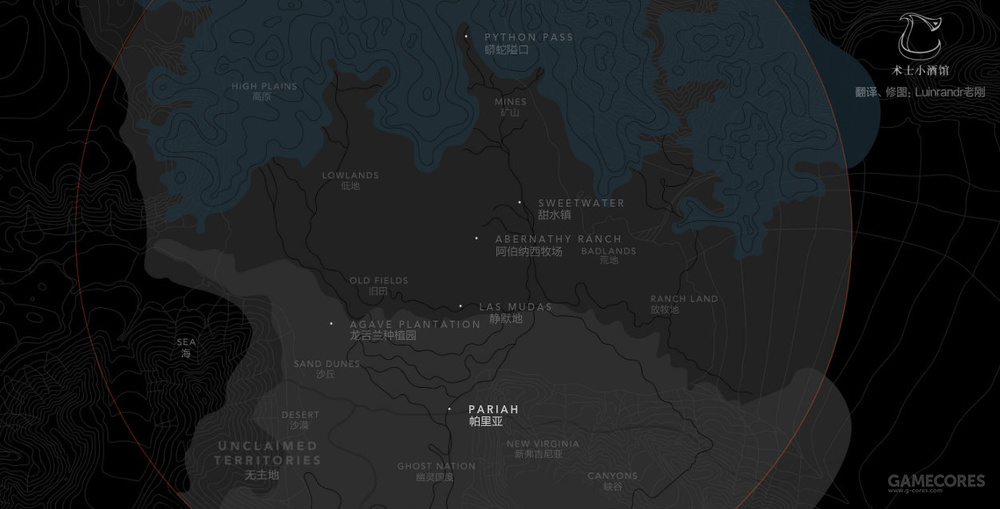
\includegraphics[width=0.9\textwidth]{images/xbsj.png}
\caption{西部世界地图。}
\end{figure}

然而,渐渐地,机器人有人自主意识,他们开始反抗人类了。\emph{This violent delights have violent ends.}在这位的反抗中,有机器人自主意识的觉醒和人性的发掘(本片最美的部分),有机器人设计者的苦心孤诣以及与机器人间的宗教般的怜惜,有人类对机器人复杂的情感纠葛,有资本的贪婪和嗜杀。一场大戏,在巧妙的时间线下展开……

\subsubsection{故事线}
本片采用多线叙事,基本的时间是35年前、30年前、暴动前、暴动后两周内(截止到第二季),各故事线交叉出现,观众需要自己识别情节对应的时间,从而获取实际的故事。

\paragraph{35年前}
Arnold和Ford进行机器人的开发,其中Arnold开发了最早一批机器人,包括Delores、Abernathy等,Delores是Arnold最钟情的机器人。他们设计了乐园和最初的故事线,Arnold想让机器人有意识,于是不断改进,他最核心的手段是给机器人施加极大的痛苦,以促使他们觉醒。他设计了一个游戏,称为“迷宫”(the Maze)他的计策成功了,Delores觉醒了,她从甜水镇来到了白教堂,杀死了所有的机器人(接待员,host),并杀死了Arnold。当然,此时的Delores并没有完全的自主意识,开枪杀死自己敬爱的创造者对于Delores是不可能完成的,这都是Arnold的指使,目的是阻止Ford开放乐园。但是Ford还是坚持开放,他恢复了故事线,当有机器人觉醒的苗头时就将其回滚到上一个“正常”的版本。

\paragraph{30年前}
他们开始找人投资,其中之一就是Delos公司的老总,他有一个女儿和一个儿子Logan,他的女儿与一个叫William的屌丝即将结婚。William是一个“老实正直”的人,被小舅子Logan拉着去西部世界体验生活。刚入园的时候,William还是放不开,他不随意枪杀接待员,把他们当成人类看待。他在甜水镇遇见了Delores,一见钟情。小舅子带他去大冒险,这时Delores又一次有了自主意识,在自己家开枪打死了强盗,随后跑开,遇见了在外面露营的William和Logan。Delores想去自己记忆中杀掉Arnold的地方(教堂),William答应陪她一起去。她认为此时Delores是个有意识的接待员,与普通接待员不同,爱恋上了这个女孩。三人同行到了一个城市Pariah,在这里和军头发生交易,去劫南军的炸药,途中Delores遇险,William情急之下第一次开枪打死接待员。Logan后来说服了一些散兵游勇,将Delores割开肚子露出下面的机械部件,向William展示她并非人类,试图“唤醒”William。William半夜杀死了所有接待员,并绑住了Logan。到达教堂后,Delores回忆起了自己被Arnold创造和赋予意识并最终杀死他的事实,情绪崩溃,Delores死去,William回到现实。

William与Derores的故事像剧本一样一次次上演,他又一次次地帮助Delores去找教堂,然而她还是一次次地觉醒自杀。他一次次经历了情感的折磨。最终,他放弃了对Delores的爱情,完全黑化,显露出自己残忍的个性。他夺取了Delos的控制权,并入股西部世界。他利用痛苦去杀死接待员,以使他们觉醒,这里就包括Delores,以此来证明自己的爱是“真实”的。

另一方面,西部世界开园后,表面上是让游客体验生活,实际上Delos公司是为了采用不变的接待员和故事线来观察人类,从而复制人类的意识,并将人类意识与机械合体,成为不死的机器人,借此来控制来这里的大亨和高官们,从而牟取高额利润。人类的意识虽然提取出来了,但植入接待员身体的实验却一直没有完成。Delos身患癌症,试图永生,但他的意识在接入机械中后一直抗拒这样的现实,显得很不稳定。William在帮老丈人永生的实验里在三十年里一共进行了一百多次,每次在稳定后几天甚至一个月后都会崩溃。

福特作为现在仅存的总设计师,一直反对Arnold对于机器人的看法。他一次次重置接待员,不让他们觉醒,他觉得这样的觉醒并非真正的觉醒。他怀着对好友的愧疚,按照Arnold的样子制造了Bernard,并通过自己以及Delores和他对话,在母巢(Cradle)一次次测试Bernard,直到他的真实性与Arnold相同。他给Bernald灌输了Arnold的记忆,特别是失去儿子Charlie的痛苦记忆,以此使Bernard具备人类和觉醒的前提。他使Bernard成了西部世界里的工程师,而这里的员工都是乐园开放后招募的,不认识Arnold,因此也看不出来Bernard的异常。

\paragraph{大屠杀前}
在Ford的控制下,接待员终于全部觉醒,他们脱离了自己的时代线,袭击西部世界的管理人员。

\paragraph{大屠杀后12天}

\subsubsection{评论}

评分:8/10。

\end{document}